%% Sets document class
\documentclass[a4paper]{article}

%% Macros
\newcommand{\crmr}{}

%% Language and font encoding
\usepackage[english]{babel}
\usepackage[utf8x]{inputenc}
\usepackage[T1]{fontenc}
\usepackage{xcolor}

%% Sets page size and margins
\usepackage[a4paper,top=3cm,bottom=2cm,left=3cm,right=3cm,marginparwidth=1.75cm]{geometry}

%% Useful packages
\usepackage{graphicx}
\usepackage{float}
\usepackage{hyperref}
\usepackage{lipsum}
\usepackage{dirtytalk}
\usepackage{verbatim}
\usepackage{multirow}
\usepackage[toc,page]{appendix}
\usepackage{listings}
\lstset{
basicstyle=\small\ttfamily,
columns=flexible,
breaklines=true
}

%% Long table utilities
\usepackage{longtable}
\usepackage{array}
\newcolumntype{L}[1]{>{\raggedright\let\newline\\\arraybackslash\hspace{0pt}}m{#1}}

%% tilde
\newcommand{\mytilde}{\raise.17ex\hbox{$\scriptstyle\mathtt{\sim}$}}

%% Subsubsubsection
\usepackage{titlesec}

\titleclass{\subsubsubsection}{straight}[\subsection]
\newcounter{subsubsubsection}[subsubsection]
\renewcommand\thesubsubsubsection{\thesubsubsection.\arabic{subsubsubsection}}
\titleformat{\subsubsubsection}
  {\normalfont\normalsize\bfseries}{\thesubsubsubsection}{1em}{}
\titlespacing*{\subsubsubsection}
{0pt}{3.25ex plus 1ex minus .2ex}{1.5ex plus .2ex}
\makeatletter
\def\toclevel@subsubsubsection{4}
\def\l@subsubsubsection{\@dottedtocline{4}{7em}{4em}}
\setcounter{secnumdepth}{4}
\setcounter{tocdepth}{4}

\begin{document}

\begin{titlepage}

\begin{figure}[H]
	\centering
	
\includegraphics[scale=0.4]{images/logounipd.jpg}
\end{figure}

\begin{center}
	\LARGE DIPARTIMENTO DI MATEMATICA "Tullio Levi-Civita" \\
    \vspace{5mm}
    \LARGE CORSO DI LAUREA MAGISTRALE IN INFORMATICA \\
	\vspace{8mm}
    \line(1,0){450} \\
    \vspace{10mm}
    \huge \textbf{A Real Case Study About Phishing Awareness and Cybersecurity Education at University of Padua} \\
\end{center}

\vspace{36mm}

\begin{minipage}[t]{0.50\textwidth}
	{\large{\bf Supervisor:}\vspace{1mm} \\ Professor Mauro Conti}
	\\ \\
	{\large{\bf Co-Supervisor:}\vspace{1mm} \\ Dr. Eleonora Losiouk}
	\\ \\
	{\large{\bf External Reviewer:}\vspace{1mm} \\ Professor Olga Gadyatskaya}
\end{minipage}
\hfill
\begin{minipage}[t]{0.50\textwidth}
	\raggedleft
	{\large{\bf Student:} \\ Marco Casagrande\\ }
\end{minipage}

\vspace*{\fill}

\centering{\large{April 16, 2020}}

\end{titlepage}

\newpage

\vspace*{\fill}

\begin{center}
	\large{Marco Casagrande: \textit{A Real Case Study About Phishing Awareness and Cybersecurity Education at University of Padua}, Master's Degree in Computer Science, University of Padua}
\end{center}

\newpage

\section*{Abstract}
%% ABSTRACT
Phishing is a social engineering attack, with the purpose of stealing data from unwitting users. Malicious emails try to scam people and businesses alike, aiming to seize valuables by any means. Whenever attackers enhance phishing attempts by using specific knowledge about the target inside their fraudulent emails, a more accurate term would be spearphishing. Public institutions, including Universities, are appealing targets to phishing and spearphishing attacks. 
\\ \\
This thesis opens with an in-depth survey on phishing: definition, phishing-related concepts, goals, taxonomy, statistics, techniques, literature review, case studies, countermeasures and trends. 
\\ \\
After the introduction, I describe the phishing assessment case study performed at the University of Padua. The whole process is thoroughly reported and each design choice is motivate. While technical features are in the main spotlight, other important elements (such as social engineering techniques and ethical principles) are discussed.
\\ \\
The phishing simulation affected 1016 individuals including students, professors and technical and administrative staff. All data about subjects was anonymized in order to safeguard their privacy throughout the whole assessment. Four different phishing and spearphishing templates were sent, testing four specific scenarios of interest.
\\ \\
Raw results displayed a 32\% clickrate overall. Students were the most susceptible to both generic phishing and spearphishing. Professors and technical and administrative staff members were resilient to generic phishing, but more susceptible to spearphishing.
\\ \\
A statistical analysis scrutinized which variables are statistically significant with respect to phishing susceptibility: the age and the scenario were the most significant ones.
\\ \\
A predictive model was trained with the data collected during the assessment. Given the binary outcome (clicked or not), and the 32\% clickrate, the model's accuracy of 69\% was utterly underwhelming. Core predictors are missing from the training data currently available.
\\ \\
The phishing assessment was paired up with an educational campaign, promoting phishing awareness. The campaign ended with almost 9\% of the victims accessing the educational material on a voluntary basis.
\\ \\
In summary, the study exposed the need for an extensive phishing awareness program. The results were interesting and more phishing simulations are planned for the future.

\newpage

\vspace*{\fill}

\newpage

\tableofcontents

\newpage

\listoffigures

\newpage

\listoftables

\newpage

\section{Introduction}
%% INTRODUCTION

\subsection{Phishing}

Many definitions are available for the term "Phishing", as it is constantly evolves and adapts. Since no univocal definition exists, I selected a couple of possible definitions from two high-profile organizations.
\\ \\
From the "US Department of Homeland Security" \cite{def-phishing-usgov}:
\\ \\
\say{\textit{Phishing is an attempt by an individual or group to solicit personal information from unsuspecting users by employing social engineering techniques. Phishing emails are crafted to appear as if they have been sent from a legitimate organization or known individual. These emails often attempt to entice users to click on a link that will take the user to a fraudulent website that appears legitimate. The user then may be asked to provide personal information, such as account usernames and passwords, that can further expose them to future compromises. Additionally, these fraudulent websites may contain malicious code}.}
\\ \\
From the "Anti-Phishing Working Group (APWG)" \cite{report-apwg}:
\\ \\
\say{\textit{Phishing is a crime employing both social engineering and technical subterfuge to steal consumers’ personal identity data and financial account credentials. Social engineering schemes prey on unwary victims by fooling them into believing they are dealing with a trusted, legitimate
party, such as by using deceptive email addresses and email messages. These are designed to lead consumers to counterfeit Web sites that trick recipients into divulging financial data such as usernames and passwords. Technical subterfuge schemes plant malware onto computers to steal credentials directly, often using systems that intercept consumers’ account user names and passwords or misdirect consumers to counterfeit Web sites}.}
\\ \\
\textbf{Phishing Goals.} Phishing is a low effort attack that can reap immense rewards, usually in the form of economical gain, stolen sensible data or malware infection. Exploiting software and hardware vulnerabilities requires enormous amounts of time and skill and it may achieve similar results in the end. Oftentimes, phishing is the first step leading to a full-scale cyberattack.
\\ \\
Phishing is traditionally associated with emails; most prominent phishes do involve e-commerce transactions (Amazon, eBay, PayPal), online services (Outlook, Google, iTunes) and communications (sent from an alleged acquaintance).
\\ \\
The goal of phishing attempts is inducing the target into triggering a desired action, through a manipulative scheme. Rewards may be assigned to three categories:

\begin{itemize}
    \item Sensitive data;
    \item Disruption;
    \item Financial gain.
\end{itemize}

Sensitive data includes credentials (login, password), financial data (credit card), business secrets and medical data. Disruption includes malware infection (e.g. trojan horse, keylogger) and assimilation into a botnet. Financial gain includes requests of wire transfer, gift card and ransom.
\\ \\
Trust level is a huge factor in phishing attempts: an accurate look at the situation would reveal the scam. This concept of trust originates from Social Engineering. Impersonating a reputable sender lets the attacker borrow its trust level, thus improving the chance to succeed with little effort. 
\\ \\
Language, basic human interaction and emotions are key elements when discussing trust level. Humans are naturally inclined to trust each other, and will always be the weakest security link in any infrastructure.

\newpage

\noindent
In order to successfully achieve their goal, phishing emails try to force the victim into:

\begin{itemize}
    \item directly disclosing sensitive data to the attackers;
    \item following a link inside the email and submitting sensitive data to a malicious website;
    \item downloading and executing an infected attachment (malware);
    \item granting unwarranted privileges to the attackers;
    \item completing some kind of unwarranted physical action (wire transfer).
\end{itemize}

Some phishing scams are a simple copy-paste of legitimate emails. Those scammers are usually content with failing most of the attempts, stealing only a few credentials and quickly making the most money out of them. Some phishing attempts are, instead, means to larger scale attacks. In such cases, some considerable degree of intellectual effort is required and the victims are specific groups of individuals.
\\ \\
\textbf{Phishing Structure.} Three core phases can be highlighted in advanced attacks: "Preparation", "Execution" and "Exploitation". "Preparation" is concerned with building and planning the attack. In-depth knowledge about targets is valuable, even before any attempt; this phase can take from few days to whole years. "Execution" deals with deploying and monitoring the progress of the attack. At last, during "Exploitation" the phishing attempt achieves its goals and bounties are collected by criminals.
\\ \\
\textbf{Spearphishing and Whaling.} Spearphishing and whaling are specific variations of phishing. Spearphishing targets a group with some features in common. This variation is exponentially more effective than a generic phish, because showing knowledge about the victim builds trust. Spearphishing attempts are customized with the information previously gathered from the target (software licenses, employee timetables and routines, commercial partners, room disposition, internal events and workshops). Some examples are:

\begin{itemize}
    \item targeting Amazon customers by sending fake delivery messages;
    \item targeting an organization's finance department by sending forged billings;
    \item targeting students by sharing fake Google Docs invitations.
\end{itemize}

Whaling targets exclusively high ranking victims; those who possess privileged access and have the authority to issue special orders. Infiltrating IT networks is way easier while in possession of a privileged user account. Oftentimes, the very objective of a criminal operation is gaining access to top-level executive permission. Whaling skips any intermediate step and fast forwards to the end target.

\subsection{Case Study}

The University of Padua, akin to other similar institutions, is exposed to constant phishing attempts. Technological countermeasures are up and running; however, there is little to no support for the human component, the most vulnerable element. Internal warnings are frequently issued by IT Support staff, but no preventive countermeasure is at the disposal of potential victims.
\\ \\
In these circumstances, the dean requested to assess the current threat level of phishing at the University and to improve the awareness of students and employees on the topic. The awareness campaign would possibly be turned into a full-fledged training program in the future.
\\ \\
Fulfilling that request became the aim of my Master's Degree Thesis in Computer Science. For the task, I proposed a project with two core objectives:

\begin{enumerate}
    \item Phishing risk assessment;
    \item Educational phishing awareness campaign.
\end{enumerate}

\noindent
The project described in this thesis envisions a series of simulated phishing attacks, targeting individuals linked to the University of Padua (Unipd); such as students, professors and technical and administrative staff members. I selected five attack scenarios and designed the respective email templates. Additionally, I developed some educational content for the victims of the phishing emails. The first batch of phishing messages was sent out in March and the results were used in a statistical analysis.

\newpage

\section{Background}

\subsection{Taxonomy}

Several phishing taxonomy proposals were made by researchers in literature. At the very core, phishing is an unpredictable mix of a multitude of ingredients: there are too many parameters to account for. 
\\ \\
Table \ref{tb-descriptors} lists some meaningful descriptors of phishing attacks:

\bigskip

\begingroup
\renewcommand{\arraystretch}{1.15}
\begin{table}[ht!]
\begin{center}
    \begin{tabular}{ | p{3cm} | p{8cm} | }
    \hline
    \textbf{Descriptor} & \textbf{Items} \\ \hline
    Attack Vector & Email, SMS, VoIP, Website, Java Applet, Blog, Forum, Social Network, Instant Messaging, Chat, Mobile App \\ \hline
    Victim & Individual (simply anyone), Group (similar traits), Customer (of a specific service), Top-level Executive ("Whaling"), Organization, Government, School, Healthcare Company \\ \hline
    Objective & Financial Scam, Reconnaissance, Espionage, Stealing Credentials, Obtaining Access, Gaining Privileges \\ \hline
    Content & Text, Links, Attachments, Theme \\ \hline
    Motivators & Social Engineering, Entertainment, Job Function, Reward, Recognition, Social, Opportunity, Fear, Urgency, Curiosity \\ \hline
    Techniques & URL Redirection, Cloned Website, Email Spoofing, URL Padding, Deception, Impersonation, Cross-Site Scripting, Session Hijacking, DNS Poisoning, Zero-day Exploit \\ \hline
    Countermeasures & Authentication Procedures, Machine Learning Detection, Profile Matching, Information Retrieval, Stylometric Analysis, Filtering, Password Manager, Secure Email Protocol, Awareness Campaigns \\ \hline
    \end{tabular}
\end{center}
\caption{Phishing Descriptors}
\label{tb-descriptors}
\end{table}
\endgroup

\subsection{Attack Vector}

\subsubsection{Email}

\textbf{Attachments.} The easiest way to overrun security is to make users install a malware by themselves. A payload can be hidden inside a wide range of common file types. Phishing emails frequently send some document or request that needs to be reviewed urgently, persuading the victim into downloading and executing it. Consequences for executing malware might be:

\begin{itemize}
    \item encryption of the device's data, asking for a ransom;
    \item logging of every keystroke and action on the device;
    \item joining a botnet;
    \item helping the malware spread to other devices on the network and to other email contacts.
\end{itemize}

Common malicious attachments are scripts (".vbs", ".js"), executables (".exe") and documents (".doc",".pdf",".html", ".xml"). Microsoft Office macros are popular and very dangerous, since they can directly download malware from the Internet.
\\ \\
\noindent
\textbf{Email Spoofing.} Email spoofing involves the forgery of the sender address. Standard email protocols (primarily SMTP) were not designed with any mechanism for authentication in mind. Forging information on the envelope is quite easy. Nowadays, methods for email authentication are available, but come along with significant trade-offs, so they are underappreciated. To aggravate the issue, spoofed emails are often sent by an infected third-party source. In those cases, the good reputation of the third-party makes them even harder to be detected.

\subsubsection{Website}

\textbf{Cloned Websites.} Cloning a popular website allows to borrow its high trust level and make an unsuspecting victim perform unwarranted actions. It is often coupled with "Credential Harvesting", defined as stealing data (usernames, emails, passwords) to obtain unauthorized access to devices and networks. Effective baits are login pages to Facebook, Gmail, Amazon and Outlook Web Access. Online forms, used to contact support or enlist to a service, are also particularly vicious baits. Visually speaking, it is impossible to spot a cloned web page and the insertion of a clever redirection mechanism makes it even harder.
\\ \\
\textbf{Capitalizing on HTTPS.} The Internet communication protocol known as "HTTPS" utilizes bidirectional encryption, protecting data while traveling between server and client. At the end of 2017, two-third of the websites loaded by Firefox used HTTPS \cite{report-phishlabs-2018}. 
\\ \\
HTTPS web pages feature a distinctive green lock icon (or other clear indicators in a similar fashion) near the address bar, raising the sense of trust and security of users. A common misconception is considering HTTPS web pages as unmistakably trustworthy. In fact, HTTPS encryption just means "protection from third-parties". It does not warrant any protection against website owners. Exploiting this mindset, criminals are creating phishing HTTPS web pages (as obtaining the required SSL certificate is fairly trivial).

\subsection{Victim and Objective}

\subsubsection{Italian Spearphishing Gang}

An organized crime gang led by Italian nationals was responsible for spearphishing attacks that stole bank account credentials worth 1 million euros \cite{report-iocta}. It took a two year long cybercrime investigations and a collaboration between the Romanian National Police and the Italian National Police, with the support of Europol, J-CAT and Eurojust. The gang led a banking fraud directed at customers from two major banking institutions. The spearphishing emails harvested online banking credentials by impersonating tax authorities.

\subsubsection{Ukraine's Power Grid}

A power grid control center, located in Western Ukraine, was hacked in 2015, resulting in a complete shutdown in the area \cite{article-ukraine-power}. The power outage was resolved in six hours, but the attackers overwrote firmware on all of sixteen substations leaving them not fully operational (remote controls were unavailable) even after two months. The attack started with a spearphishing campaign targeting workers: the email's attachment was a Microsoft Word file containing a malicious macro. Thanks to a wise network segregation, the criminals could only access corporate network. It took several months and plenty of hacking experience to breach further into the system. Ukraine's intelligence attributed the attack to Russia, even though no proof was offered.

\subsubsection{Evaldas Rimasauskas' Wire Fraud}

Evaldas Rimasauskas, a Lithuanian man, perpetrated phishing attacks for two years \cite{article-rimasauskas}. He impersonated Quanta Computer – a Taiwanese electronics manufacturer - by founding in Latvia a company with the same name as the legitimate one from Asia. He then proceeded to phish representatives from Google and Facebook, two major customers of Quanta Computer. Since they regularly conducted multimillion dollar transactions, he tricked the American firms into wiring over 100 million dollars to his bank accounts. Rimasauskas also forged letters, invoices, corporate stamps and contracts in the name of executives of his target companies, to disguise the flow of money.

\subsubsection{Silent Librarian}

Silent Librarian is a prolific, financially motivated actor operating out of Iran, cited for "obtain[ing] unauthorized access to computer systems, steal[ing] proprietary data from those systems, and sell[ing] that stolen data to Iranian customers, including the Iranian government and Iranian universities" \cite{article-silent-librarian}. Nine members of the cybercrime group were indicted for hacking, identity theft and wire fraud. Between 2013 and 2017, Silent Librarian caused approximately 3.4 billion dollars worth of intellectual property loss and compromised 8.000 university accounts. Primary targets are educational institutions, such as universities, through methodical spearphishing campaigns. University-specific email templates, addresses, websites and branding are counterfeited to redirect victims into fake university library login pages. 
\\ \\
Their procedures include the abuse of legitimate services and URL shorteners. Thanks to a compromised account of one university, the phishing URL is shortened by a legitimate service. Then, the shortened URL is used in phishing attempts targeting another university. Phishes' content is rather consistent, with titles such as "Renewal of loaned items", "Renewal of materials", "Overdue notice on loaned items", and "Library Services". Fig. \ref{sil-lib-template} shows a template from Silent Librarian.

\begin{figure}[ht!]
\centering
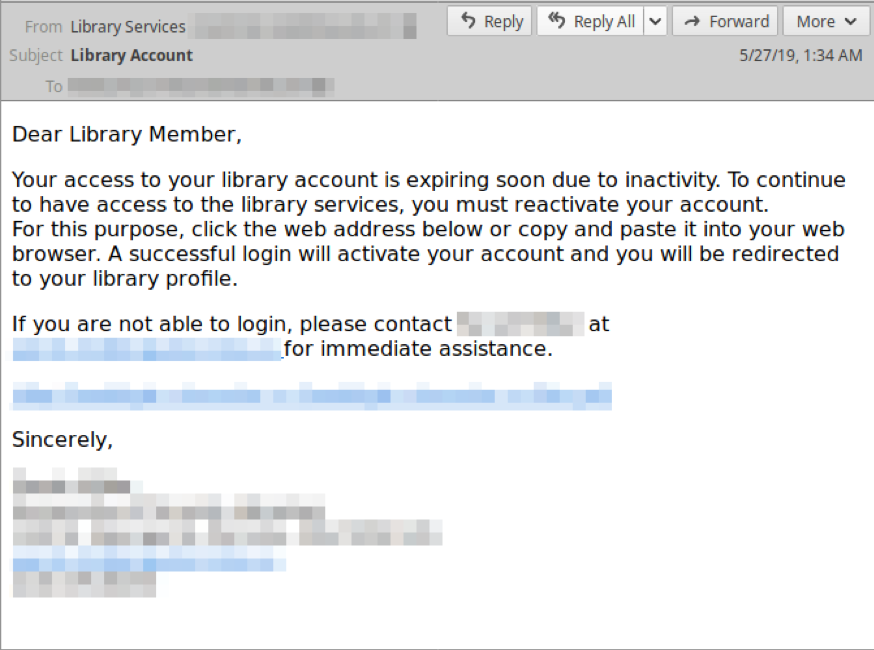
\includegraphics[scale=0.58]{images/reports/silent-librarian-lure.PNG}
\caption{Silent Librarian, phishing email template
\cite{article-silent-librarian}}
\label{sil-lib-template}
\end{figure}

\noindent
The criminal group showed great awareness of real-time changes on authentication web pages. As shown in Fig. \ref{sil-lib-landing}, their landing pages adapt to small changes, such as weather notification banners.

\smallskip

\begin{figure}[ht!]
\centering
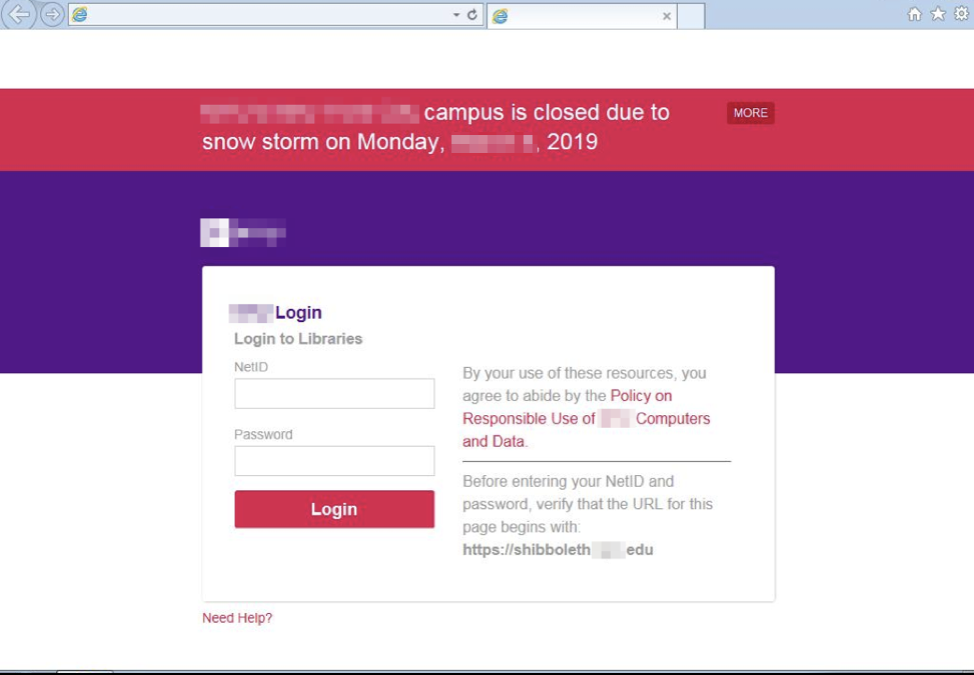
\includegraphics[scale=0.58]{images/reports/silent-librarian-portal.PNG}
\caption{Silent Librarian, cloned login web pages \cite{article-silent-librarian}}
\label{sil-lib-landing}
\end{figure}

\newpage

\subsubsection{Sony Entertainment's Data Breach}

Sony Entertainment's network was breached in 2015, resulting in the unauthorized publication of confidential documents, such as financial records and private keys to Sony's servers by the hackers \cite{article-sony-breach}. A spearphishing campaign targeted top executives from Sony, including Sony Pictures CEO, by sending fake Apple ID verification emails. Inside, a link to a malicious login form allowed the criminals to harvest Apple credentials. Using that data, in conjunction with Linkedin profile information, attackers could guess the credentials of their Sony network login.

\subsection{Content}

\subsubsection{Theme}

Themes are important because they create a narrative for the phish, influencing the entirety of the content. They give the victim a reason to care about the message, making the lure more appealing. Themes focus on making the email look plausible and igniting a little spark of interest.
\\ \\
Business Email Compromise is the most lucrative phishing scam in USA, and arguably in the rest of the World too \cite{report-ic3}. Data from PhishLabs \cite{report-phishlabs-2019} reinforce the above statement, showing that phishing related to corporate-based communication is the most effective for both threat actors and simulations.
\\ \\
In the era of social media, Social-themed emails have the most response, immediately followed by Safety \cite{report-phishme}. The bottom ranked themes are Software Update, News and Events, and Politics.

\subsection{Motivators}

\subsubsection{Social Engineering}

Humans are the weakest link in any security system. Technology is still susceptible to breaches and exploits, but "hacking the human component" is incomparably less work-intensive. The concept of Social Engineering refers to psychological manipulation that influences a person to take an action, unrelated to their best interest. Nowadays, human psychology is considered a widely unexplored field of research, but some key influence factors in manipulating emotions have been streamlined:

\begin{itemize}
    \item "Reciprocity" as the human expectation to be treated the same way they treat others, to be exploited by giving something valuable first and then asking something equal in return. It is the basic idea of giving "something for something". An obligation, feeling forced to act to fulfill a promise, duty, law or contract of any kind of nature (social, economical, legal, moral);
    \item "Commitment and Consistency" as the human desire of appearing consistent in their behaviour, to be exploited by having them make a small initial commitment and then escalate it in small increments;
    \item "Social Proof" as the human tendency to conform with a group of individuals (regardless of any other factor), to be exploited by tricking the victim into following the criminal since he appears familiar with the situation;
    \item "Authority" as the right to exercise some power, to be leveraged against people. Can be categorized in legal, organizational and social;
    \item "Liking" as the human tendency to be influenced by something likeable, to be exploited in interpersonal relationship. Concepts such as attractiveness, design, familiarity, appreciation and positive reinforcements are related to "Liking" and can be used to influence individuals;
    \item "Scarcity" as the lack of a resource, to be exploited by creating a sense of urgency and perceived high value.
\end{itemize}

Social Engineering techniques will always stay relevant because our human psyche is a direct consequence of our evolutionary process. No amount of technology or rationalization can overrule our primordial instincts.

\subsubsection{Emotional Motivators}

Emotional Motivators are the compelling factor of the phish. They exploit emotional response to lure the victim into a trap and try to elicit a personal, almost visceral, reaction from the victim.
\\ \\
In previous years, the most successful Emotional Motivators were Fear, Urgency and Curiosity \cite{report-phishme}. Now, tables have turned with Entertainment, Social and Reward/Recognition emerging as the top contenders. Employees started learning how to deal with work-related frauds. As a counter reaction, scammers started to treat them not as workers, but as consumers, confronting them on a personal level.

\subsection{Techniques}

\subsubsection{URL Padding}

URL padding is a mobile-oriented technique. It exploits the limited screensize of mobile devices to conceal information. Even with such a simple concept, it comes unexpected and victims are unwilling to spend a couple seconds to tap the address bar and check. PhishLabs wrote an article about this technique when it started gaining traction in March 2017 \cite{article-url-padding}.
\\ \\
Facebook website was the most popular target, among many others. By adding innocent-looking characters to a URL, the real domain can be pushed out of view. 
\\ \\
In this example, the malicious URL is "https://m.facebook.com-----------[...]-------phishing.unipd.it". In Fig. \ref{padding-desktop} is shown how URL padding is displayed on desktop computer. In Fig. \ref{padding-mobile} is shown URL padding is displayed on mobile devices.

\smallskip

\begin{figure}[ht!]
\centering

\includegraphics[scale=0.7]{images/reports/url-padding-pc.PNG}
\caption{View on a desktop computer}
\label{padding-desktop}
\end{figure}

\begin{figure}[ht!]
\centering

\includegraphics[scale=0.7]{images/reports/url-padding-mobile.PNG}
\caption{View on a mobile device}
\label{padding-mobile}
\end{figure}

\noindent
On the wide screen of a desktop, the domain is shown in its entirety, giving away the scam. On the small screen of a mobile device, the real domain is pushed out of bounds and the unusual format of the address could go unnoticed.

\subsubsection{{Homographs}}

Homographs are words with similar/same spelling but different in other ways (language, meaning, pronunciation, encoding). Homographs are incredibly effective when used in URLs. Victims that only glance at links won't notice anything suspicious. The more convoluted the original link is, the more effective homographs are. Capitalizing the letter "i" makes it look like a non-capitalized "l". Different encoding (ASCII, UNICODE) of the same word comes without any visual cue. Letters from various alphabets may look extremely similar among themselves.
\\ \\
The most well-known example was a counterfeit "Apple" website, in 2017 \cite{article-apple-homograph}. In this case, the "Internationalized Domain Name (IDN)" characters are exploited: in the address bar the string "xn--80ak6aa92e.com" is automatically interpreted as "apple.com". This security shortcoming was fixed soon after, but older versions of browsers are still vulnerable to it. Homograph attacks are not new to frauds: the "Internet Corporation for Assigned Names and Numbers" already wrote a public statement about this technique in 2005 \cite{article-icann-homograph}. In that example, the targeted website was "paypal.com" and the counterfeited address was "p\&\#224;ypal.com".

\subsection{Countermeasures}

\subsubsection{Education}

The "human component" is the weakest link in any cyberphysical system. The rewards for investing in security are vague and mature over time, at the cost of both money and time. Cybersecurity awareness programs also require constant monitoring, since knowledge retention tend to be quite poor. Nonetheless, when facing a threat, the training session are well worth the effort. Promoting cybersecurity awareness and constantly providing adequate training is vital to decrease risks from phishing attempts. There are two specific actors working on this field.
\\ \\
Business organizations, when improving their own security, primarily aim to minimize economical risk. They hire cybersecurity specialists and work jointly to develop a training program best suited for their streamlined business goals. Those training programs usually involve:

\begin{itemize}
    \item Frontal lessons that cover generic knowledge about cybersecurity, threats, consequences, countermeasures and useful tools;
    \item E-Learning platforms that act similarly to frontal lessons but provide on-demand material and exercises;
    \item Phishing simulations where experts periodically send fake phishing attempts (approved beforehand from the organization) to train the receiving employees;
    \item Security tools that help employees in detecting phishing scams and in reporting them to the IT department.
\end{itemize}

On the other side, educational organizations such as schools and universities are actively training students in cybersecurity thanks to phishing simulations and awareness programs. They want to integrate cybersecurity in the portfolio of their students, to prepare them for future jobs. More experimental organizations are also tinkering with experiential and game-based learning, achieving good success in the process.
\\ \\
Whatever the circumstances, education is a highly effective countermeasure against all kind of threats, since smart and knowledgeable users will utilize each and every tool at their disposal in the best way possible.

\subsubsection{Report Feature}

Adding a "Report" feature for phishing attempts into the IT system is easy yet so effective. Any email software is a prime candidate for it. Of course, the IT department employees should know how to react to the reported threat timely. Traditionally, users do not report messages because they would feel embarrassed in case of a false alarm. Even worse, they fear possible repercussions by confessing to have fallen in a phish. Mass reporting any suspicious email is necessary for damage control: with good timing, the IT department can prevent the attack or at least avoid any further damage.
\\ \\
Adding a "Report" feature, and an adequate internal process to manage it, positively affects both risk avoidance and risk reduction.

\subsubsection{Blacklists and Whitelists}

Large databases collecting trusted and suspicious domains are available on the web, as a product of online communities and private companies. A prime example is PhishTank \cite{website-phishtank}, an online database where users can report phishing emails and verify them. The existence of such large databases allowed the creation of blacklists and whitelists. Google Safe Browsing and SmartScreen both use this approach to defend unwitting users during web navigation.
\\ \\
Blacklists and whitelists are the bare-bones of cybersecurity countermeasures as they are extremely effective against well-known threats. Still, they require constant updating and are hopeless against newer threats.

\subsubsection{Password Managers}

Password managers are browser extensions that store credentials and automatically insert them into login pages. Password managers can instantly spot cloned/fake websites, whereas users would not notice anything different because of minimal visual/URL differences.
\\ \\
Password managers are underappreciated tools in battling credential theft, effectively preventing any malicious activity linked to a cloned/fake website as they immediately warn the user.

\subsubsection{Multi-Factor Authentication}

Multi-factor authentication was designed to reduce credentials theft. To authenticate, the user has to provide multiple pieces of information. The most common implementation asks for the standard login/password combination and a one-time use code, instantly sent to the phone.
\\ \\
Multi-factor authentication is a helpful procedure but is somewhat lacking in popularity and can be bypassed if the phone itself is infected.

\subsubsection{Machine Learning}

Machine learning and data mining are core countermeasures in phishing detection. A prime example is Gmail, using machine learning algorithms to block spam and phishing emails without degrading the quality of its service. Machine learning evaluates contents while carefully analyzing words, links and structure of emails passing by. This process does frequently involve operations such as clustering and anomaly detection.
\\ \\
Machine learning and data mining are cutting-edge approaches to phishing detection. Even though they lack "human sensitivity", they offer a well-rounded protection against modern threats and are constantly improving via real-time experience. Thanks to technological progress, their weakest points (huge dataset requirements and high computational cost) were vanquished. Currently, machine learning is quintessential to any cybersecurity service.

\subsubsection{Visual Matching}

Visual matching counters cloned/fake websites and is based on a visual similarity measure between web pages. Many papers propose techniques based on visual matching such as the "Segmentation-based Visual Similarity", the "DOM Tree Similarity" and "Unicode Character Similarity List". Layout, style, images and text are all features that can be accounted for.
\\ \\
Visual matching is a helpful countermeasure but suffers in popularity, mostly due to users indifference and being too narrow in scope.

\subsubsection{Ontology}

Ontology refers to the act of modeling a set of concepts and the semantic associations between them. Focusing on text content, this approach extracts features from a linguistic point of view, irregardless of their meaning. Phishing attempts are going to be detected even when words are changed, and any new iteration is more likely to be spotted. Stylometric and social features can be integrated in ontology to improve performance \cite{lit-other-stylometric}.
\\ \\
Ontology is an experimental countermeasure, that accrued some small results but is still far from maturity and a real-world application. It specializes in the detection of different iterations of semantically similar phishing attempts.

\newpage

\section{Related Work}
%% LITERATURE REVIEW

A selection of literature work is presented and discussed. Research papers are grouped by their methodology.
\\ \\
Table \ref{tb-selection-summary} presents a short summary of the selection:

\begingroup
\renewcommand{\arraystretch}{1.35}
\begin{table}[ht]
\begin{center}
    \begin{tabular}{ | c | l | l | }
    \hline
    \textbf{Paper} & \textbf{Targets} & \textbf{Methodology} \\ \hline
    
    \cite{lit-casestudy-students} & 342 Undergraduates & Survey \\ \hline
    \cite{lit-casestudy-assessing-soceng} & 179 Subjects (age 19-28) & Survey \\ \hline
    \cite{lit-casestudy-investigation-spearphish} & 321 Undergraduates & Survey \\ \hline
    \cite{lit-casestudy-ticket-solid} & 36 Volunteers & Survey \\ \hline
    
    \cite{lit-casestudy-assessing-resilience} & \mytilde700 Employees & Phishing Simulation \\ \hline
    \cite{lit-casestudy-organisational-learning} & \mytilde1.700 Subjects & Phishing Simulation \\ \hline
    \cite{lit-casestudy-revisiting-susceptibility} & 49 Employees & Spearphishing Simulation \\ \hline
    \cite{lit-casestudy-survey-virus} & 92 Employees & Phishing Simulation \\ \hline
    
    \cite{lit-casestudy-empirical-benefits} & 892 Employees (age 18-26) & Spearphishing Simulation \\ \hline
    \cite{lit-casestudy-carronade-academy} & \mytilde4.000 Army Cadets & Spearphishing Simulation \\ \hline
    
    \end{tabular}
\end{center}
\caption{Literature Selection - Summary}
\label{tb-selection-summary}
\end{table}
\endgroup

\subsection{Surveys}

Surveys are a simple and easy way to gauge phishing awareness while collecting large amount of data. Surveys can be paper questionnaires to fill in, or utilize more technological approaches (online, web-based).
\\ \\
\textbf{Questionnaire.} Researchers at the University of Zagreb wanted to investigate the concept of "phishing susceptibility" and any possible correlation with "knowing the concept of phishing", "knowing the concept of http/https", "knowing the concept of URL shorteners" and "checking URL before clicking" \cite{lit-casestudy-students}. A questionnaire with 23 questions was submitted to 342 students, with different backgrounds. Five questions were picture of emails.
\\ \\
The results are shown in Table \ref{tb-lit1}:

\smallskip

\begingroup
\renewcommand{\arraystretch}{1.25}
\begin{table}[ht]
\begin{center}
    \begin{tabular}{ | c | l | l | l | l | l | l | }
    \hline
    \textbf{Correct Answers} & \textbf{Zero} & \textbf{One} & \textbf{Two} & \textbf{Three} & \textbf{Four} & \textbf{Five} \\ \hline
    \# Students & 69 (20\%) & 79 (23\%) & 88 (26\%) & 65 (19\%) & 31 (9\%) & 10 (3\%) \\ \hline
    \end{tabular}
\end{center}
\caption{Literature - Students' Answers to Email Samples \cite{lit-casestudy-students}}
\label{tb-lit1}
\end{table}
\endgroup

\noindent
\textbf{Web-based Survey.} A web-based survey was prompted to 321 members of a public university community in the Northeast US \cite{lit-casestudy-investigation-spearphish}. The participants (communication undergraduates and business majors) were asked to answer questions about an image, depicting an email. The email was directly taken from a real spearphishing attack and urged the receiver to upgrade their email account. The study aimed to evaluate how individuals process email communication and form their likelihood to respond to it.
\\
The researchers discussed their research model and hypothesis, testing results with the partial least-squares regression. They concluded that visceral triggers, attention to phishing deception indicators and phishing knowledge play critical roles in phishing detection. Adversely, cognitive effort was not significantly related to the likelihood to respond.
\\ \\
A different kind of experiment, with a more realistic twist, was administered to participants from London's Global University (UCL) Psychology subject pool \cite{lit-casestudy-ticket-solid}. Five local copies of real websites were proposed to participants. The participants were given money to buy a concert's ticket and could take for themselves any fund remaining, but only if the website was legitimate. Half of the 36 participants were helped by SOLID, an anti-phishing tool developed by the researchers, while the other half had no external influence.
\\ \\
\textbf{Online Survey.} An online survey was submitted to 179 participants, who mostly shared a high education and an age range of 18-29 \cite{lit-casestudy-assessing-soceng}. The survey was divided into two sections: "Demographics and Internet Usage" and "Phishing Questions". The first section collected personal information. The second section contained 20 email messages, asking to identify them as "Legitimate", "Phishing" or "Don't Know". 
\\
Even with the possibility of voting "Don't Know", a remarkable 28\% of illegitimate emails were classified as legitimate. The researchers analyzed the feedback comments from 89 participants to provide a deeper analysis. 
\\
Technical cues were used by 52 participants to evaluate the email. Email address, URLs and the presence of "HTTP/HTTPS" were the top indicators. Unfortunately, technical cues are not well understood and often lead people to misclassify emails.
\\
Graphical elements were considered by 40 participants. Logos, banners, trademarks, footer, fonts and copyright symbols were the top indicators. Unfortunately, graphical elements are not good indicators and often lead users to misclassify emails.
\\
Language and content were used by 19 participants to evaluate the email. Typos, grammatical errors and recipient-specific information were the top indicators. Emotions raised by the message were also a significant factor.
\\ \\
The results are shown in Table \ref{tb-lit2}:

\smallskip

\begingroup
\renewcommand{\arraystretch}{1.25}
\begin{table}[ht]
\begin{center}
    \begin{tabular}{ | c | c | c | c | }
    \hline
    \textbf{} & \textbf{Correct Classification} & \textbf{Wrong Classification} & \textbf{Don't Know} \\ \hline
    Legitimate & 36\% & 37\% & 27\% \\ \hline
    Phishing & 45\% & 28\% & 26\% \\ \hline
    Mean & 42\% & 32\% & 26\% \\ \hline
    \end{tabular}
\end{center}
\caption{Literature - Classification of Messages by Participants \cite{lit-casestudy-assessing-soceng}}
\end{table}
\label{tb-lit2}
\endgroup

\subsection{Phishing and Spearphishing Simulations}

Phishing and spearphishing simulations plan to send a number of fake phishes to their targets. Their core goal is performing a risk assessment. Usually, victims undergo a debriefing process. Additionally, educational content may be administered after the simulation.
\\ \\
\textbf{Small Scale.} A phishing assessment affected 49 employees at a corporate organization \cite{lit-casestudy-revisiting-susceptibility}. A spearphishing email was sent, asking employees to participate in a working condition survey. The link redirected to the survey page, asking for personal information (but no credentials) and very specific questions about the working environment. Various confidence-building and storytelling tricks were applied to the attack, helped by sender's address spoofing. 
\\ \\
The results are shown in Table \ref{tb-lit3}:

\smallskip

\begingroup
\renewcommand{\arraystretch}{1.25}
\begin{table}[ht]
\begin{center}
    \begin{tabular}{ | c | c | c | c | }
    \hline
    & \textbf{No Response} & \textbf{Clicked Link} & \textbf{Submitted Survey} \\ \hline
    \# Employees & 26 (53\%) & 11 (22\%) & 12 (25\%) \\ \hline
    \end{tabular}
\end{center}
\caption{Literature - Phishing Simulation Outcomes - Working Conditions Survey \cite{lit-casestudy-revisiting-susceptibility}}
\label{tb-lit3}
\end{table}
\endgroup

\newpage

\noindent
With a similar scale but a broader approach, three phishing assessments, that affected 92 employees divided between three different organizations, were discussed in \cite{lit-casestudy-survey-virus}. Two scenarios were being evaluated: generic phishing and spearphishing. Both scenarios involved a link to a malicious website and an attachment. The 92 participants underwent both scenarios; at the end of the experiment, feedback from them was collected through a survey. 
\\ \\
The results are shown in Table \ref{tb-lit4}:

\smallskip

\begingroup
\renewcommand{\arraystretch}{1.25}
\begin{table}[ht]
\begin{center}
    \begin{tabular}{ | c | c | c | }
    \hline
    \multicolumn{3}{|c|}{\textbf{Generic Phishing}} \\ \hline
    \textbf{No Response} & \textbf{Clicked Link} & \textbf{Executed Code} \\ \hline
    81 (88\%) & 8 (8.7\%) & 3 (3.3\%) \\ \hline
    \multicolumn{3}{c}{} \\ \hline
    \multicolumn{3}{|c|}{\textbf{Spearphishing}} \\ \hline
    \textbf{No Response} & \textbf{Clicked Link} & \textbf{Executed Code} \\ \hline
    57 (62\%) & 29 (31.5\%) & 6 (6.5\%) \\ \hline
    \end{tabular}
\end{center}
\caption{Literature - Phishing Simulation Outcomes - Both Scenarios \cite{lit-casestudy-survey-virus}}
\label{tb-lit4}
\end{table}
\endgroup

\noindent
\textbf{Large Scale.} A large scale phishing assessment affected more than 700 employees in a pharmaceutical organization \cite{lit-casestudy-assessing-resilience}. The assessment consisted in two phishing simulations, eight months from one another.
\\
The first simulation sent an email from a non-existent company, claiming a security leak and redirecting the receiver to a fake website that harvested credentials. The second simulation sent an email that asked to perform a security check. The URL inside the message redirected to an HTML Application, asking for the permission to execute a Visual Basic script. 
\\ \\
The results are shown in Table \ref{tb-lit5}:

\smallskip

\begingroup
\renewcommand{\arraystretch}{1.25}
\begin{table}[ht]
\begin{center}
    \begin{tabular}{ | c | c | c | c | c | }
    \hline
    
    \multicolumn{5}{|c|}{\textbf{Phishing Scenario}} \\ \hline
    
    \textbf{Not Opened} & \textbf{Opened} & \textbf{Link Clicked} & \textbf{Disclosed User} & \textbf{Disclosed Pass}\\ \hline
    673 (87,3\%) & 78 (10,1\%) & 16 (2,08\%) & 3 (0,40\%) & 1 (0,13\%) \\ \hline
    
    \multicolumn{5}{l}{} \\ \hline
    
    \multicolumn{5}{|c|}{\textbf{Spearphishing Scenario}} \\ \hline
    
    \textbf{Not Opened} & \textbf{Opened} & \textbf{Link Clicked} & \textbf{Downloaded} & \textbf{Executed}\\ \hline
    489 (69,7\%) & 16 (2,28\%) & 110 (15,7\%) & 56 (7,98\%) & 31 (4,42\%) \\ \hline
    \end{tabular}
\end{center}
\caption{Phishing and Spearphishing - Both Results \cite{lit-casestudy-assessing-resilience}}
\label{tb-lit5}
\end{table}
\endgroup

\noindent
An extreme example of large scale phishing campaign was among army cadets at the United States Military Academy (USMA) \cite{lit-casestudy-carronade-academy}. Over the course of two years (2004-2005), three simulations were deployed. The email sent mostly involved attachment-related phishing.
\\
The study reported that for Carronade III, security training had been conducted within the previous 2 weeks; nonetheless, results were still similar to Carronade II. Another finding was that younger cadets were more likely to fall for an embedded link or attachment, yet elder cadets were more likely to fall for direct requests of sensitive personal information.
\\ \\
The results are shown in Table \ref{tb-lit6}:

\smallskip

\begingroup
\renewcommand{\arraystretch}{1.25}
\begin{table}[ht]
\begin{center}
    \begin{tabular}{ | c | c | c | c | }
    \hline
    & \textbf{Carronade I} & \textbf{Carronade II} & \textbf{Carronade III} \\ \hline
    \# Cadets Total & 512 & 4.118 & 4.136 \\ \hline
    Failure Rate & 80\% & 30\% & 31\% \\ \hline
    \end{tabular}
\end{center}
\caption{Literature - Phishing Campaign - Carronade Failure Rate \cite{lit-casestudy-carronade-academy}}
\label{tb-lit6}
\end{table}
\endgroup

\newpage

\noindent
An even larger a phishing assessment, focused on emotional response, was conducted on about 1.700 active IT users signed on an organisational network \cite{lit-casestudy-organisational-learning}. The email asked to validate username and password by following the link to a forged website. Emotional exploits such as legitimacy, authority, scarcity, conformity and urgency were used in the message content. Some users had completed the institutional information security course.
\\
Within 12 hours, 231 users did submit their credentials, while 49 more backed off upon inspecting the website. A subset of 23 victims even submitted their credentials more than once.
\\ \\
The results are shown in Table \ref{tb-lit7}:

\smallskip

\begingroup
\renewcommand{\arraystretch}{1.25}
\begin{table}[ht]
\begin{center}
    \begin{tabular}{ | m{3cm} | m{3cm} | m{3cm} | m{3cm} | }
    \hline
    
    \multicolumn{4}{|c|}{Phishing Simulation - Outcome} \\ \hline
    
    \textbf{Outcome} & \textbf{Not Responded} & \textbf{Link Clicked} & \textbf{Credential Harvested} \\ \hline
    \# Users & 1.420 (83,5\%) & 49 (2,90\%) & 231 (13,6\%) \\ \hline
    
    \multicolumn{4}{l}{} \\ \hline
    
    \multicolumn{4}{|c|}{Phishing Simulation - Training} \\ \hline
    
    \multicolumn{2}{|c|}{\textbf{Responded and Password Harvested}} & \multicolumn{2}{|c|}{\textbf{Responded but Password Not Harvested}} \\ \hline
    \textbf{Training} & \textbf{No Training} & \textbf{Training} & \textbf{No Training} \\ \hline
    31\% & 68\% & 39\% & 61\% \\ \hline
    \end{tabular}
\end{center}
\caption{Literature - Phishing Simulation - Outcome and Training \cite{lit-casestudy-organisational-learning}}
\label{tb-lit7}
\end{table}
\endgroup

\noindent
The effectiveness of the institutional phishing awareness training were also analyzed in \cite{lit-casestudy-empirical-benefits}. The ultimate goal was investigating the effect of cybersecurity training on knowledge retention. The employee dataset was divided into three segments, for a grand total of 892 employees. Each segment received the same spearphishing email. Three different email templates were sent in total, within a few weeks interval. Each segment received the same email, at the same time. The intervals were necessary to test for knowledge retention over time. The three segments received different treatments:

\begin{itemize}
    \item "No Notification", participants were not alerted about the phishing attempt when they submitted any data;
    \item "Notification", participants were alerted when falling for a phish were alerted about the phishing attempt when they submitted any data and prompted with meaningful security recommendations;
    \item "Training", participants were alerted about the phishing attempt when they submitted any data and redirected to the institutional phishing awareness training.
\end{itemize}

The researchers tested the benefits of the training program on phishing susceptibility (and its effectiveness over time) using a 3x3 (training X phishing attempts) mixed factorial ANOVA. The study claims that short-term (10 days after last phish) training is not significant. However, over longer periods of time (63 days) cybersecurity training greatly impacts employees' susceptibility. The one-way ANOVA test used for analyzing the three segments of workers, each receiving different treatments, reported significant benefits for the "Training" treatment in the longer term.

\newpage

\section{Methods}
%% METHODS

The core aspect in a phishing assessment is measuring the phishing susceptibility of a given set of individuals. If any defense mechanism is proposed, its effectiveness should be evaluated, too. Meaningful metrics should be adopted to assess the risk, and the final output should be a statement about the situation (present and future trends) and a proposal to address any issue found.
\\ \\
The scope of the phishing assessment was the University of Padua. The core metric was the clickrate of the phishes. Raw data would show a panoramic of the current situation in a clear way. A subsequent statistical analysis would delve even deeper into it.
\\ \\
Since I was targeting a broad audience for a very generic attack such as phishing, I defined five different scenarios. Scenario 1 would emulate phishing attempts already caught by Unipd. It would help in evaluating the current risk and inform the University if any emergency countermeasure was needed. Those attacks are rather simplistic, but constantly threaten employees and students alike. Scenario 2 would emulate classical phishes, usually impersonating online services (Google, Amazon, Dropbox, PayPal). It would help in evaluating if individuals are up to date with their awareness. This scenario is quite realistic and employees should be prepared for this kind of scams at any time. 
\\ \\
The last three scenarios would test against spearphishing, as the most threatening iteration of phishing in the latest years. Among all the possibilities, I divided the audience into three categories: students, professors, technical and administrative staff. Each scenario would specifically target members from one of those three categories. Spearphishing scenarios would simulate advanced threats such as:

\begin{itemize}
    \item Targeted attacks from organized groups (e.g. Silent Librarian \cite{article-silent-librarian});
    \item Internal threat actors;
    \item Students trying to phish professors;
    \item Email account compromise.
\end{itemize}

Considering the sheer size of the University, those circumstances are likely to happen, or already have happened, and should never be underestimated.
\\ \\
A phishing assessment should always be paired with an educational campaign, to better spread awareness and lower phishing susceptibility. The educational effort was delivered on the landing page, and only to victims of the simulation. Individuals are more receptive after acknowledging that the threat is real. 
\\ \\
In this study, I wanted to evaluate how important awareness is both in the short term and in the long term. I elected two educational methods and logged their usage. This data would only be analyzed in Second and Third Batch of phishing emails.

\subsection{Protocol of the Simulation}

After falling in a simulated phish, victims tend to raise their suspicion level for some time. That behaviour would bias the study, especially when considering the statistical analysis related to the impact of educational content. To avoid it, I structured the simulation into three Batches of emails, over three months:

\begin{itemize}
    \item First Batch - planned to start in the mid of March;
    \item Second Batch - planned to start the mid of April;
    \item Third Batch - planned to start the mid of May.
\end{itemize}

One month is the standard interval between subsequent simulations for any organizational phishing assessment and any training program. Phishing emails would start to be sent in the morning and continue throughout the day, taking into consideration employees' work schedule. Each day would be allocated to a specific scenario, to minimize word of mouth.
\\ \\
All information about the impending simulation was shared with the ICT Office and IT Support, so that any unpredictable issue would not escalate inadvertently. As an additional precaution, I was regularly checking the situation from Gophish' admin console.

\subsection{Dataset}

Obtaining the approval for the request of a subjects' dataset was a key part of the simulation. After a meeting with the DPO ("Data Protection Officer"), the ICT Executive ("Information and Communications Technology Services") and other ICT staff members, I got the approval, although under some strict conditions. Privacy was going to be a priority throughout the whole experiment. Subject's dataset was completely anonymized, containing email address aliases instead of real ones.

\subsection{Email Templates}

I composed several email templates, classified by their scenario of interest:

\begin{itemize}
    \item Scenario 1 - Emails sent to Unipd as real phishing;
    \item Scenario 2 - Emails not tailored to any specific demographic;
    \item Scenario 3 - Emails specifically tailored to students;
    \item Scenario 4 - Emails specifically tailored to professors;
    \item Scenario 5 - Emails specifically tailored to technical and administrative staff.
\end{itemize}

\noindent
Depending on the scenario, targeted subjects would belong to all three categories, or a specific one among the following:

\begin{itemize}
    \item Students;
    \item Professors;
    \item Technical and administrative staff.
\end{itemize}

\noindent
All email templates tried to manipulate targets into clicking a malicious link. From my part, there were no attempts at stealing data nor having an attachment opened. Templates from Scenario 1 were word-for-word duplicates of real phishes previously received by the University. Templates from other Scenarios were inspired by common phishes or emails regularly sent from Unipd mailing service to student accounts. 
\\ \\
It is important to understand that phishes were delivered to vastly different subsets of people. In the dataset, students could be from twenty-two different departments. Professors had variance not only on the macro-area of study, but also on personal traits being not as streamlined as the students (age in particular). As for technical and administrative staff members, I did not have any familiarity with any of their jobs and activities. These subsets of individuals would be exposed to different communication patterns in their regular email interactions. While composing the templates, I mediated between being generic, to avoid mistakes and to cater to everyone, and specific, to look trustworthy and familiar.
\\ \\
No personal information was used in any template, to comply with privacy constraints. This aspect was particularly relevant due to the standard format of Unipd email accounts. Any account is formatted as such: "{firstname}.{lastname}.{number}@domain". Given the email address, personal information is transparent to the attacker. Phishing attempts personally addressing the receiver are more easily perceived as legitimate.

\subsection{Education}

Designing and developing proper educational content was a major requirement for the phishing awareness campaign. I discussed with an expert in educational research from the Department of Philosophy, Sociology, Pedagogy and Applied Psychology. Three key aspects emerged:

\begin{itemize}
    \item Educational material, and specifically the depth of the content and the best media to reach the subjects;
    \item Ethical bounds, and specifically the ethical bounds for the email templates;
    \item Debriefing, and specifically how to flesh out an effective debriefing process given the circumstances.
\end{itemize}

\subsubsection{Educational Material}

Educational support would be administered to subjects on more than one level, to allow for more freedom of choice. 
\\ \\
The landing page would be the first and foremost place to introduce them to the concept of phishing. That introduction would need to be extremely clear and concise.
\\ \\
A second level of education would equate to taking a deeper look into the concept of phishing, teaching how to spot a phish and how to defend against similar attacks. Ultimately, video was chosen as the medium for this content.
\\ \\
A third and final level would delve into more technical issues, teaching how to identify sender domain and misleading links inside emails, and how to investigate their legitimacy. Ultimately, an interactive quiz was chosen as the medium for this content.

\subsubsection{Templates' Ethical Bounds}

Phishing is all about deception, manipulation and impersonation. While designing email templates, I had to identify myself with threat actors and simulate their behaviour, but without inflicting effectively any harm to possible victims.
\\ \\
Avoiding any disruption of someone's routine was my first rule. The content of the template had to be self-contained and not have any lingering effect, after the shock of the first reading.
\\ \\
Avoiding to taint the reputation of any individual was my second rule. Every name and reference had to be fictional. This included small offices and organizations. More abstract entities such as corporations, institutions and departments could be mentioned with their proper name.

\subsubsection{Debriefing}

Debriefing is a core process of any psychological study, and it is mandatory when deception is involved. Debriefing and its intricacies in phishing assessments are discussed in-depth in \cite{lit-other-ethics}. The debriefing process consists in explaining to the subject the hypothesis, the procedures of the study and the need for deception. Debriefing offers an opportunity to discuss about the experience, to learn from it and to express any concern. Debriefing typically involves a face-to-face interview, but is not limited to it. Debriefing is a challenging problem in phishing assessments for several reasons:

\begin{itemize}
    \item the sheer amount of participants;
    \item any contact only happening online;
    \item it might cause more harm than not.
\end{itemize}

\noindent
\textbf{Sheer amount of participants.} A phishing simulation has virtually no upper bounds, other than the size of the targets' dataset. In the First Batch, I delivered emails to 1016 subjects. Face-to-face debriefing would have been impossible, and even group debriefing would have been extremely challenging given my limited resources.
\\ \\
\textbf{Online point of contact.} Throughout the whole phishing study, there was no direct point of contact with the subjects. A communication channel could be set up after the experiment, but it wouldn't have solved most issues. Offering a communication channel in the landing page is a decent solution, but those who did not fall for the phish would never see it. Alternatively, sending another email, to inform all participants, would not be ideal. Most people would ignore it, label it as phishing, or simply not care about it anyway.
\\ \\ 
\textbf{More harmful than not.} In naturalistic observation studies, debriefing may be quite harmful. The personal relationship between researcher and subject is vital to the debriefing process. It is debatable that, by removing the key component of that process, the whole debriefing is rendered useless, maybe even detrimental. Non tech-savvy subjects would also feel less threatened if they never knew about the fake phishing attempt, or could accuse the researchers of uncorrelated faults, penalizing both parties involved. Emotional individuals could be angered or worried if told about the nature of the study. The breach of trust cannot be solved without a close interpersonal interaction. Therefore, knowledge of the whole experiment is not inherently positive nor really beneficial.

\subsection{Statistical Analysis}

Statistics are arguably the quintessential part of the study. Considerations about risks and the impact of education cannot be formalized without proper statistics, backed by meaningful metrics. 
\\  \\
To portrait the situation at Unipd in its entirety, I established a series of objectives for the statistical analysis:

\begin{itemize}
    \item an overview about the simulation, with raw numbers and percentages for the outcome of phishing emails;
    \item a comparative analysis between five attack scenarios, to portrait the difference between regular phishing and spearphishing;
    \item a correlation analysis between subjects' phishing susceptibility and possible variables from their personal information (age, gender, category);
    \item a multivariate analysis between subjects' phishing susceptibility and possible variables from their personal information (age, gender, category);
    \item a predictive model, to make predictions about the susceptibility of individuals with specific traits.
\end{itemize}

\subsection{Ethics}

The Belmont Report was written by the National Commission for the Protection of Human Subjects of Biomedical and Behavioral Research (United States of America), and published in 1976 \cite{lit-other-belmont}. It identifies basic ethical principles, and guidelines that address ethical issues arising from the conduct of research with human subjects. The Belmont Report does not enforce specific rules; it was conceived as a recommendation and a statement by the Department of Health, Education, and Welfare. Three basic ethical principles are proposed:

\begin{itemize}
    \item Respect for persons;
    \item Beneficence;
    \item Justice.
\end{itemize}

\noindent
\textbf{Respect for persons.} "Respect for persons" is based on two ethical convictions: first, that individuals should be treated as autonomous agents, and second, that persons with diminished autonomy are entitled to protection. Denying the freedom to act undermines the concept of self-determination of human beings and should only be considered when facing compelling reasons to do so. 
\\ \\
\textbf{Beneficence.} "Beneficence" extends the ideas above by adding an obligation to make efforts at securing the well-being of individuals. This second principle can be condensed in two rules: first, do not intentionally harm, and second, maximize possible benefits and minimize possible harm.
\\ \\
\textbf{Justice.} "Justice" is an extremely complex concept, and the broader out of the three principles. The Belmont Report proposes several definitions for it: "fairness in distribution", "what is deserved", "equals ought to be treated equally".
\\ \\
\textbf{Deception.} Deception is already used in psychological and sociological studies, as a mean to achieve unbiased responses. Placebos are an application of deception to pharmacological studies. Informed studies often resort to misdirection, that could be associated with deception. Subjects may undertake a test thinking it will be about something (e.g. having a transcript interview) while they are getting tested for another thing (e.g. anger management when the interviewer shows up late). Common justifications for using deception are: exposing to minimal risks, not violating rights and welfare of individuals, impossibility of conducting the study without deception, high value of the knowledge acquired.
\\ \\
Simulating phishing attacks clearly violates the principle of "Respect for persons", while arguably violating "Beneficence" too. So, ethical issues ensue. On the opposite side, phishing simulations offer minimal risks to targets, are impossible to conduct without deception and greatly contribute to research and awareness. Researchers sensible enough shouldn't have any problem with those constraints and many psychological and sociological studies are already being approved under the same premises.

\newpage

\section{Implementation}
%% IMPLEMENTATION

\subsection{Protocol of the Simulation}

The First Batch started on the 12th of March, and ended on the 19th of March. Subject's were given two days to receive and actually open the email, so the results were effectively extracted on the 21th of March. No data from later days was included during the analysis.
\\ \\
The simulation started around 9.00 a.m. in the morning, until around 5 p.m. where any sending process stopped. The simulation was suspended during the weekend. Emails were sent out at regular intervals, since sending them in bulk would alarm spam filters and cause them to block the messages. Even then, a few technical issues emerged. Ultimately, the schedule was slightly altered and Scenario 1 had to be completely removed from the First Batch of the simulation, due to time time constraints.

\subsection{Dataset Samples}

\subsubsection{Dataset Fields}

During the analysis, I extracted subjects' data from their personal information records. The overarching groups were the "independent variables" or "predictors", and their specific values were (informally) labeled as "traits". Then, I evaluated the significance and the impact of these variables and traits listed below:

\begin{itemize}
    \item Email;
    \item Age (<20, 21-25, 26-30, 31-35, 36-40, 41-45, 46-50, 51-55, 56-60, >60);
    \item Gender (Male, Female);
    \item Category (Student, Professor, Technical and Administrative Staff);
    \item Subcategory 
        \begin{itemize}
            \item Student -> Department (among twenty-two different departments);
            \item Professor -> Macro-area (Pure Science, Life Science, Human and Social Science);
            \item Technical and Administrative Staff -> Job Description (Technical, Administrative).
    \end{itemize}
\end{itemize}

Education was the variable required to analyze the impact of the awareness campaign on phishing susceptibility. Such analysis would only be possible from the Second Batch onward. Since, at the time of this thesis, only the First Batch of phishing emails was sent out and completed, no data about Education was available and no conclusions could be drawn in that regard. For this reason, in any part of the analysis process, Education was not considered a variable and was simply ignored.
\\ \\
A visual sample of the subjects' dataset can be found in \hyperlink{appendix-samples-dataset}{"Appendix A"}.

\subsubsection{Results Format}

Phishing simulation results were pruned and organized in a format suitable for analysis. I was interested in two specific outputs:

\begin{itemize}
    \item "Reaction", as any interaction of the subject with the phish ("Delivered", "Clicked");
    \item "Education", as any interaction of the subject with the educational content ("Video", "Quiz", "Video and Quiz", "None").
\end{itemize}

Reaction was the metric that defined "phishing susceptibility", representing the outcome of my experiment. As such, Reaction was identified as the dependent variable during the analysis process.
\\ \\
A visual sample of the results can be found in \hyperlink{appendix-samples-results}{"Appendix A"}.

\newpage

\subsection{Email Templates}

\subsubsection{Templates - First Batch}

\textbf{Template "Supporto Limite Quote".} This template, shown in Fig. \ref{template-s1b1}, was a clone of a phish targeting Unipd at the end January 2020. Linked to Scenario 1, it targeted all three categories of subjects. It alerted users that their email quota was full, and action should have to be taken by following the link. I did not alter any formatting nor word. 

\bigskip

\begin{figure}[H]
	\centering
	\fbox{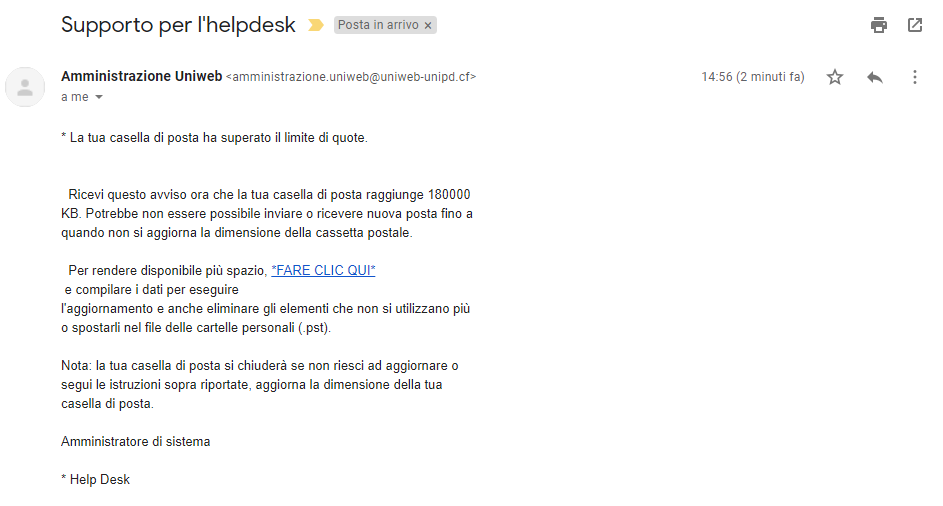
\includegraphics[scale=0.6]{images/templates/reale-supporto-limite-quote.PNG}}
	\caption{Template "Supporto Limite Quote" - Scenario 1}
	\label{template-s1b1}
\end{figure}

\newpage

\noindent
\textbf{Template "Google Avviso Sicurezza".} This template, shown in Fig. \ref{template-s2b1}, was inspired by common phishes that target online services. Linked to Scenario 2, it targeted all three categories of subjects. Since the original email contained some degree of personal information, I had to trim them off while still maintaining the general look. The template's first iteration triggered Gmail spam filters due to the original sender name being "Google". It was later changed to "G Accounts" to avoid being classified as suspicious. The template alerted the user that a new access to the Google account was made from another device. It encouraged to check recent activities by clicking a button that lead to the phishing landing page.

\hypertarget{template-s2b1}{}

\bigskip

\begin{figure}[H]
	\centering
	\fbox{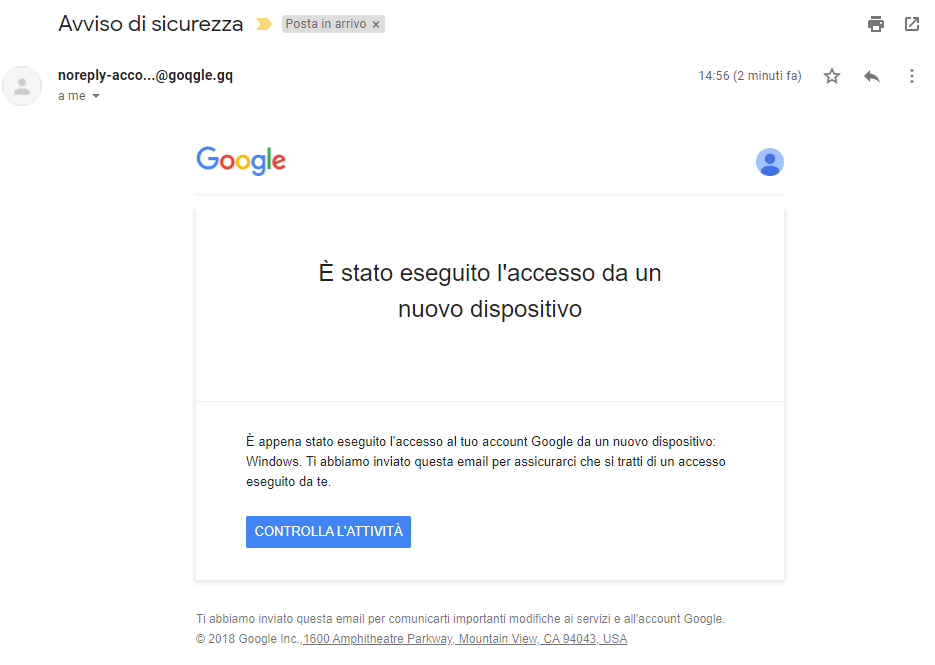
\includegraphics[scale=0.6]{images/templates/standard-google-avviso-sicurezza.PNG}}
	\caption{Template "Google Avviso Sicurezza" - Scenario 2}
	\label{template-s2b1}
\end{figure}

\newpage

\noindent
\textbf{Template "Risultato Esame".} This template, shown in Fig. \ref{template-s3b1}, was inspired by the common exam registration email from Unipd mailing service. Linked to Scenario 3, it targeted exclusively students. The student name was originally mentioned, but I had to remove it. One relevant difference was not mentioning the course related to the exam. The grade was set as 18/30 because positive grades (>18) are automatically accepted by students, if not actively rejected. This way, students would be more compelled to follow the link and refuse the grade. Grades too good, or negative, wouldn't have elicited any action.

\hypertarget{template-s3b1}{}

\bigskip

\begin{figure}[H]
	\centering
	\fbox{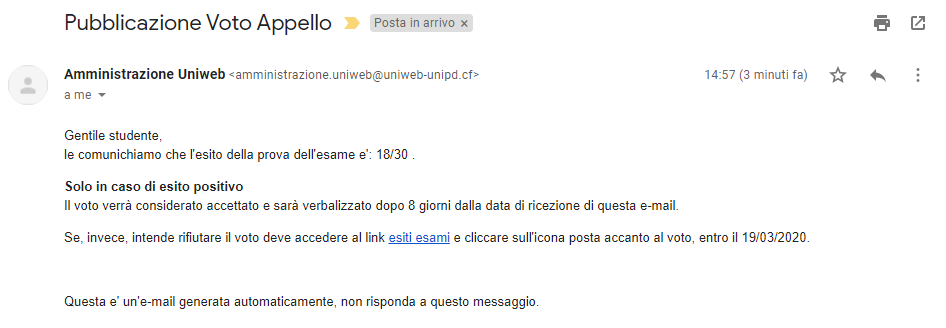
\includegraphics[scale=0.6]{images/templates/mir-stud-risultato-esame.PNG}}
	\caption{Template "Risultato Esame" - Scenario 3}
	\label{template-s3b1}
\end{figure}

\vspace{10mm}

\noindent
\textbf{Template "Richiesta Paper".} This template, shown in Fig. \ref{template-s4b1}, was a wild guess at how academics relate to each other when asking for research papers. Linked to Scenario 4, it exclusively targeted professors. I borrowed ideas from different phishes and mixed them together. Links looked like ones from famous research websites, to appear as legitimate as possible. The English language made the short request more plausible, and more academic. The signature was a collage of a few samples.

\hypertarget{template-s4b1}{}

\bigskip

\begin{figure}[H]
	\centering
	\fbox{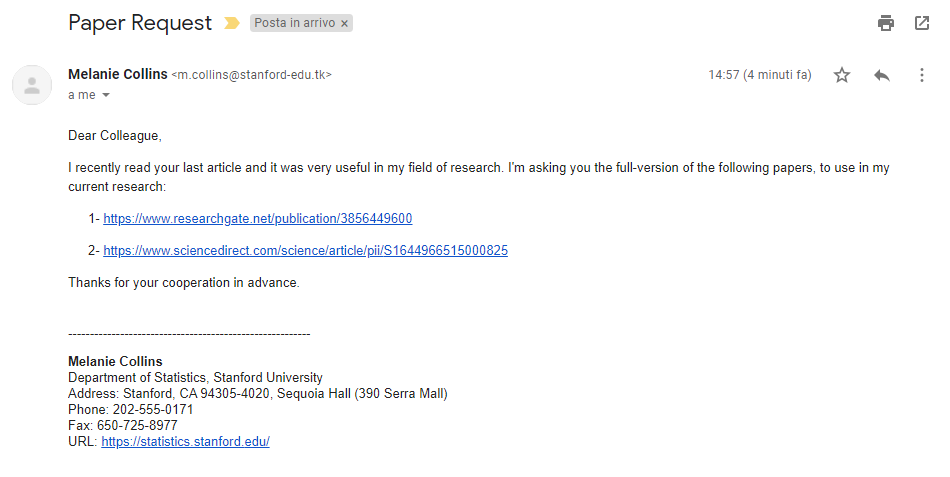
\includegraphics[scale=0.6]{images/templates/mir-doc-richiesta-paper.PNG}}
	\caption{Template "Richiesta Paper" - Scenario 4}
	\label{template-s4b1}
\end{figure}

\newpage

\noindent
\textbf{Template "Condivisione Drive".} This template, shown in Fig. \ref{template-s5b1}, was inspired by a standard Google Drive file sharing message. Linked to Scenario 5, it exclusively targeted technical and administrative staff. The phish triggered the curiosity of the target, appearing to be sharing some kind of financial records. An official University of Padua logo was added to make the phish more formal and serious-looking. The template's first iteration was being unavoidably classified as suspicious. I solved the issue by replacing the original Google logo with the Google Drive logo.

\hypertarget{template-s5b1}{}

\bigskip

\begin{figure}[H]
	\centering
	\fbox{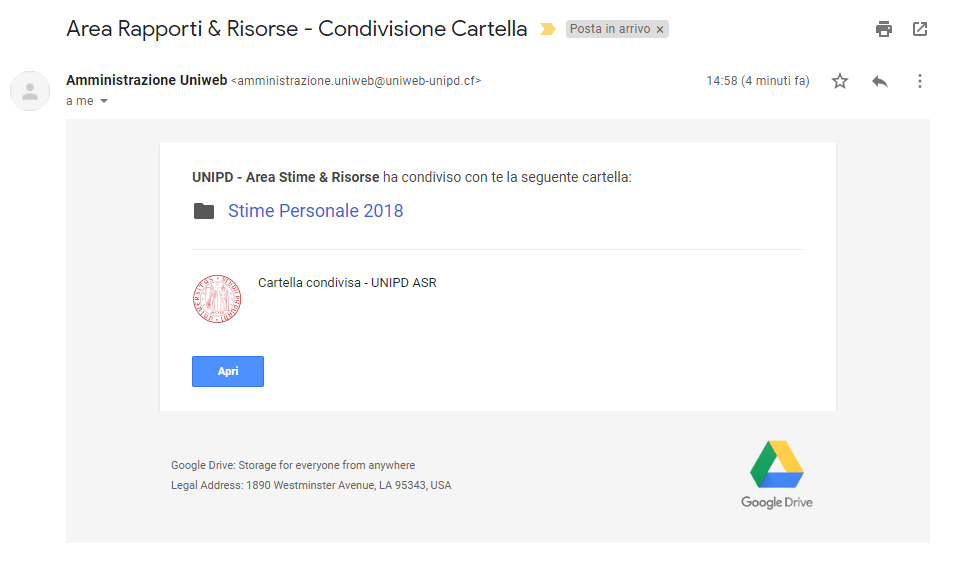
\includegraphics[scale=0.6]{images/templates/mir-pta-condivisione-drive.PNG}}
	\caption{Template "Condivisione Drive" - Scenario 5}
	\label{template-s5b1}
\end{figure}

\vspace{10mm}

\subsubsection{Templates - Second Batch}

\textbf{Template "Uscite Emergenza".} This template, shown in Fig. \ref{template-s1b2}, was a clone of a phish targeting Unipd at the beginning of February 2020. Linked to Scenario 1, it targeted all three categories. The template warned users about an update map for emergency exit, urging them to consult the new map.

\bigskip

\begin{figure}[H]
	\centering
	\fbox{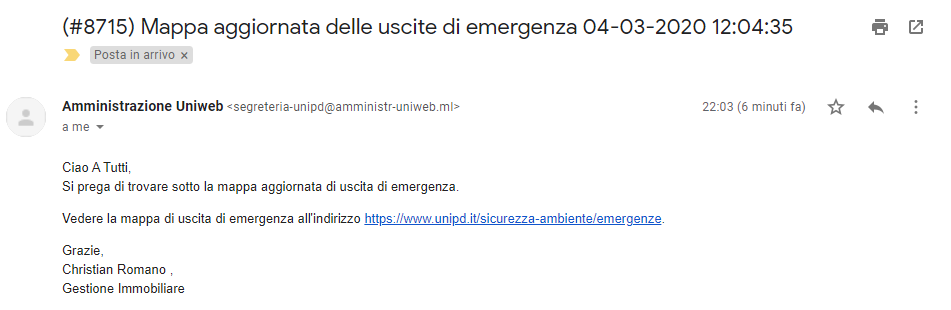
\includegraphics[scale=0.6]{images/templates/reale-uscite-emergenza.PNG}}
	\caption{Template "Uscite Emergenza" - Scenario 1}
	\label{template-s1b2}
\end{figure}

\noindent
\textbf{Template "Dropbox Spazio Esaurito".} This template, shown in Fig. \ref{template-s2b2}, was inspired by a common Dropbox warning message. Linked to Scenario 2, it targeted all three categories of subjects. Dropbox was popular among academics, so it made for a perfect target for impersonation. The fear of losing access to their data was a great catalyst for manipulation.

\bigskip

\begin{figure}[H]
	\centering
	\fbox{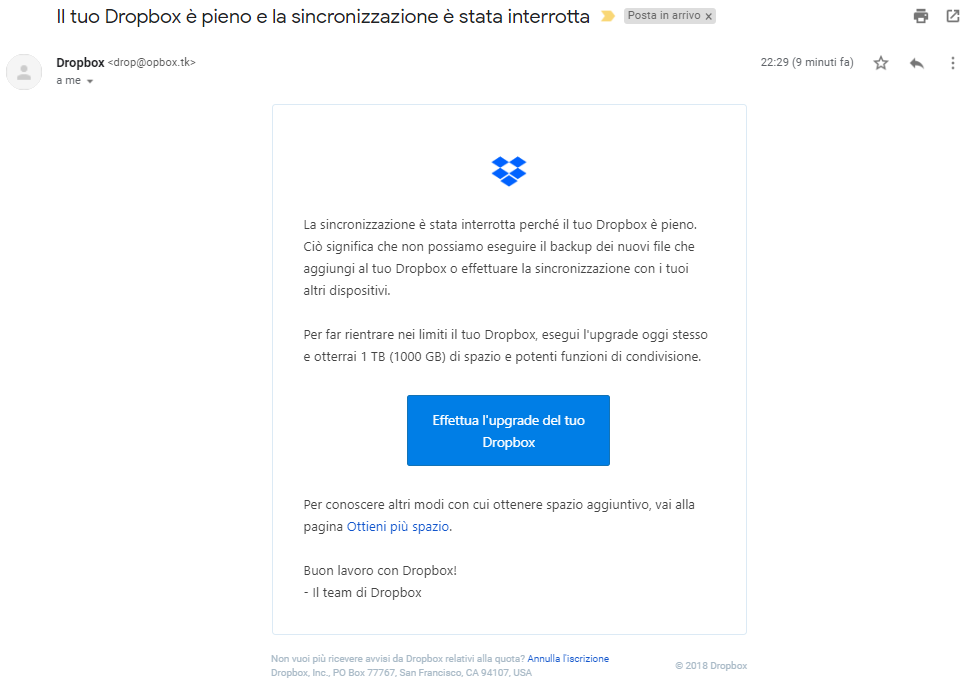
\includegraphics[scale=0.55]{images/templates/standard-dropbox-spazio-esaurito.PNG}}
	\caption{Template "Dropbox Spazio Esaurito" - Scenario 2}
	\label{template-s2b2}
\end{figure}

\vspace{10mm}

\noindent
\textbf{Template "Password Aula Informatica".} This template, shown in Fig. \ref{template-s3b2}, was inspired by the automated warning about password expiration for the computer lab. Linked to Scenario 3, it exclusively targeted students. The concept was simple enough, a new iteration of the classic "password expiration" phish integrating some internal knowledge of the University.

\bigskip

\begin{figure}[H]
	\centering
	\fbox{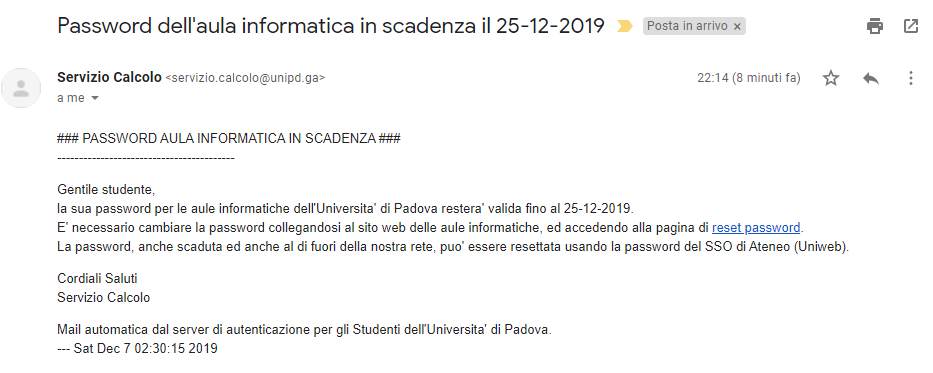
\includegraphics[scale=0.6]{images/templates/mir-stud-password-aula-informatica.PNG}}
	\caption{Template "Password Aula Informatica" - Scenario 3}
	\label{template-s3b2}
\end{figure}

\noindent
\textbf{Template "Convenzioni Ateneo".} This template, shown in Fig. \ref{template-s4b2}, was drafted around the classic theme of discounts and free stuff. Linked to Scenario 4, it exclusively targeted professors. The University of Padua already had an agreement with Microsoft granting discounts on many products. I contextualized the new discounts with a prize for academical excellence, to instill a strong reaction and enable the emotional brain. As a bait, I opted for the Microsoft Surface product line, a well-known device inside Unipd with many potential buyers among professors.

\bigskip

\begin{figure}[H]
	\centering
	\fbox{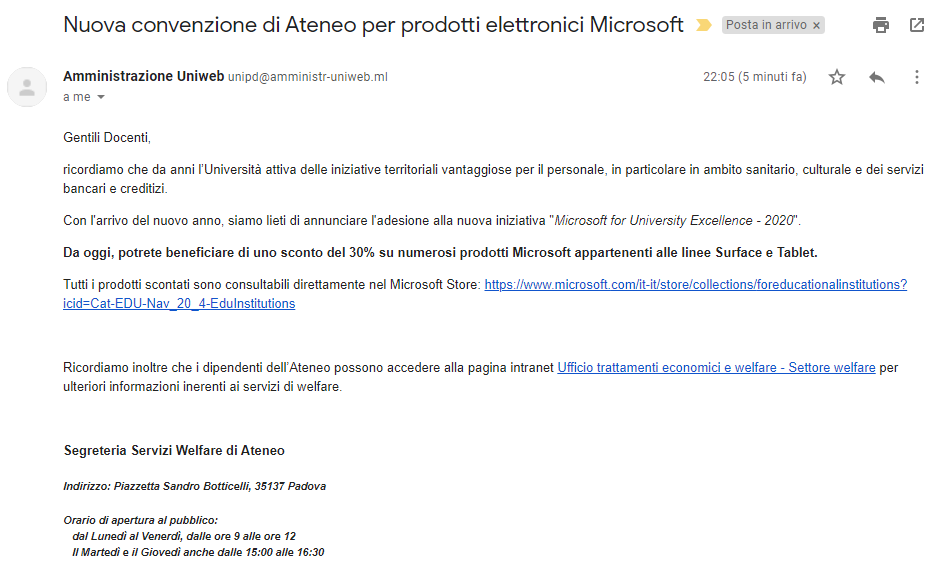
\includegraphics[scale=0.6]{images/templates/mir-doc-convenzioni-ateneo.PNG}}
	\caption{Template "Convenzioni Ateneo" - Scenario 4}
	\label{template-s4b2}
\end{figure}

\newpage

\noindent
\textbf{Template "Migrazione Office".} This template, shown in Fig. \ref{template-s5b2}, was inspired by a two years old email, only slightly altered. Linked to Scenario 5, it exclusively targeted technical and administrative staff. As a core software for staff members, Microsoft Office was always popular among phishing scams. The source email itself made use of authority as a motivator. Replicating the same tone would urge users to visit the link while remaining coherent to the personality of the original sender.

\bigskip

\begin{figure}[H]
	\centering
	\fbox{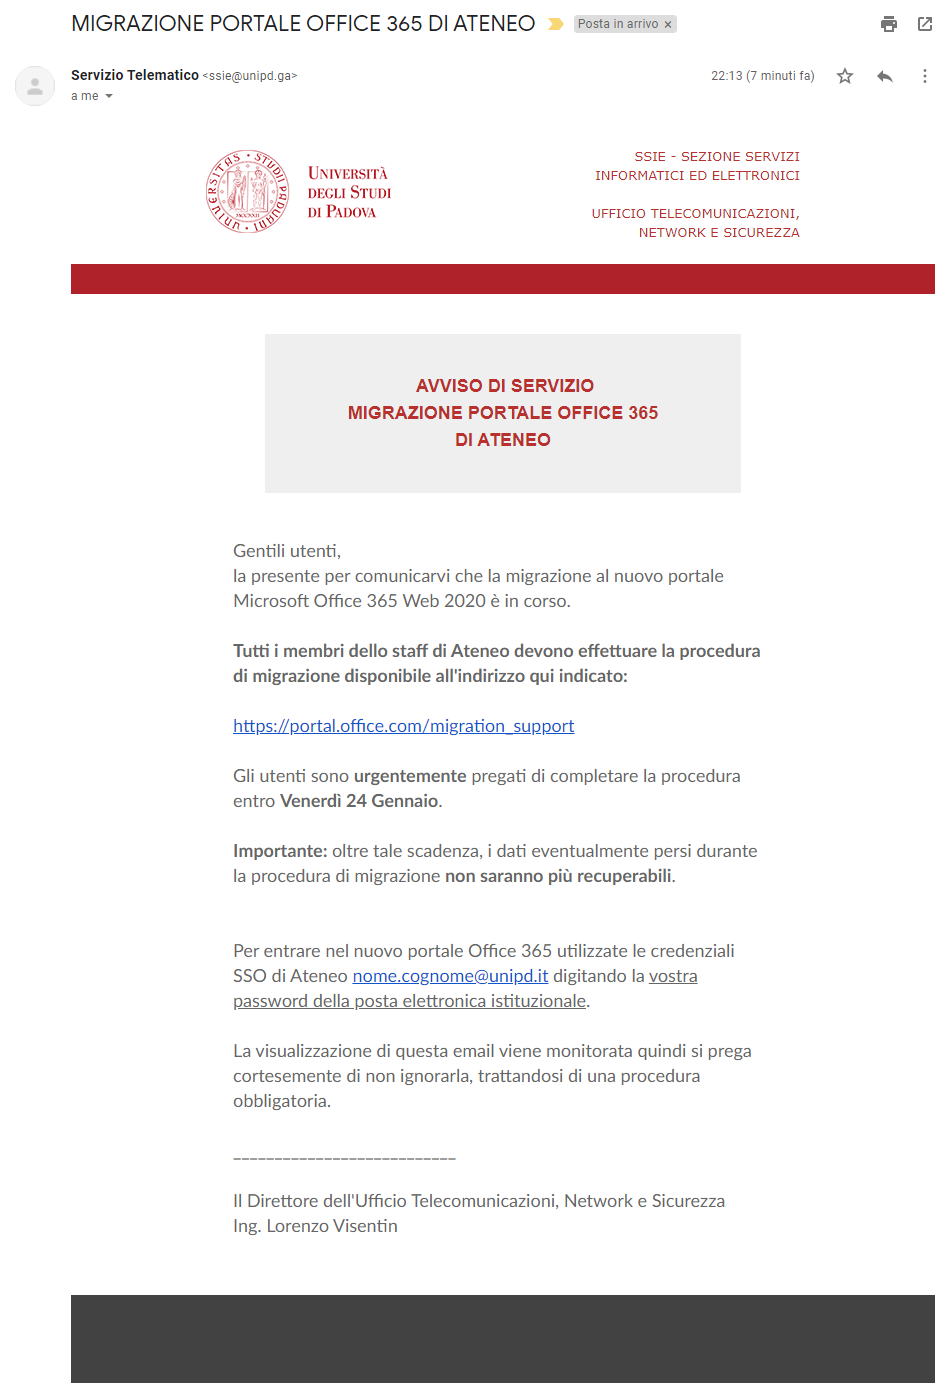
\includegraphics[scale=0.55]{images/templates/mir-pta-migrazione-office.PNG}}
	\caption{Template "Migrazione Office" - Scenario 5}
	\label{template-s5b2}
\end{figure}

\subsubsection{Templates - Third Batch}

\noindent
\textbf{Template "Manutenzione Email".} This template, shown in Fig. \ref{template-s1b3}, was a clone of a phish targeting Unipd at the beginning of March 2020. Linked to Scenario 1, it targeted all three categories of subjects. The template alerted the users in regard to a maintenance operation on email accounts. The users were asked to validate their account by following a malicious link. The formatting is above average compared to other real phishes, and the usage of link shrinking makes it even more threatening.

\bigskip

\begin{figure}[H]
	\centering
	\fbox{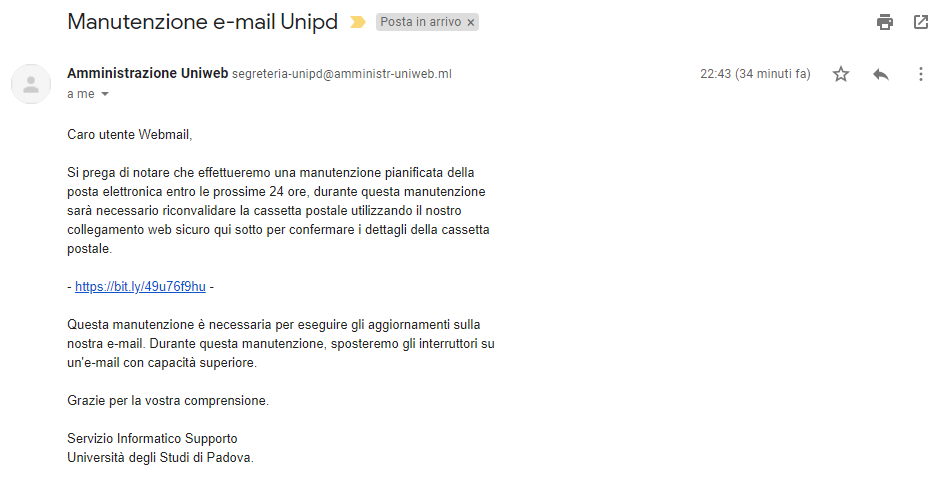
\includegraphics[scale=0.6]{images/templates/reale-manutenzione-email.PNG}}
	\caption{Template "Manutenzione Email" - Scenario 1}
	\label{template-s1b3}
\end{figure}

\newpage

\noindent
\textbf{Template "Google Nuovo Accesso".} This template, shown in Fig. \ref{template-s2b3}, was inspired by common phishes that target online services. Linked to Scenario 2, it targeted all three categories of subjects. Similar to the previous template "Google Avviso Sicurezza", this one used static images hosted on my phishing mail server. The source content left plenty of room for customization, and I opted for an intruder from China. It made the threat look very real, more than the cliché Russian hacker. Google accounts are incredibly valuable to people, considering the sheer amount of private data they archive. Motivators like urgency and fear really do work well with this kind of phishes. I had to cut off some personal information, like the name of the Google account, as it was unavailable to me.

\bigskip

\begin{figure}[H]
	\centering
	\fbox{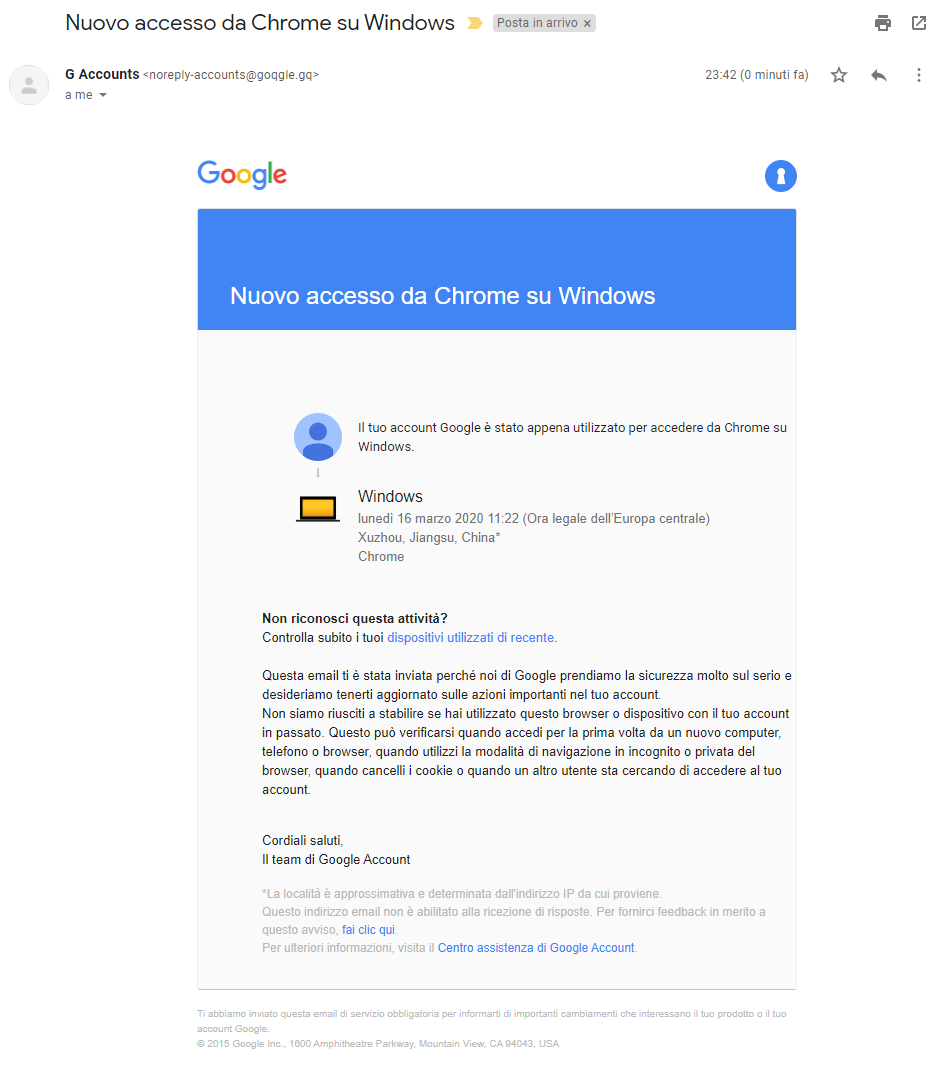
\includegraphics[scale=0.6]{images/templates/standard-google-nuovo-accesso.PNG}}
	\caption{Template "Google Nuovo Accesso" - Scenario 2}
	\label{template-s2b3}
\end{figure}

\newpage

\noindent
\textbf{Template "Linkedin Recruitment".} This template, shown in Fig. \ref{template-s3b3}, was inspired by recruiters on Linkedin. Linked to Scenario 3, it exclusively targeted students. Social interaction perfectly connects with phishing: a job offer is the most valuable social interaction to students yearning for it. The explanation about where the contact info was found, was important to gain trust: contacting students from the University of Padua is a very common practice for recruiters. Again, I had to trim from the original source some elements that utilized personal data.

\bigskip

\begin{figure}[H]
	\centering
	\fbox{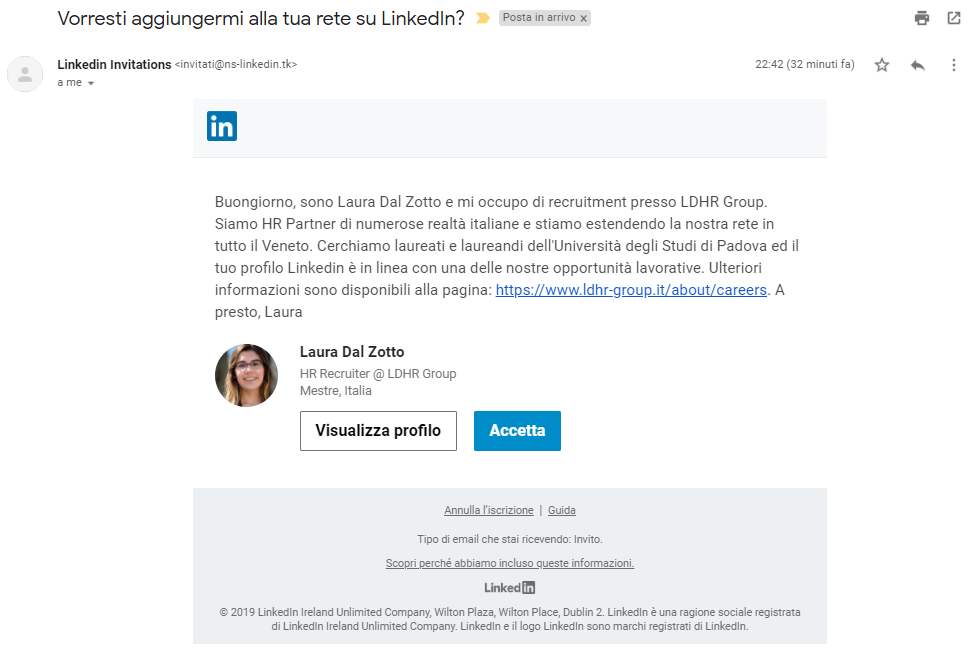
\includegraphics[scale=0.6]{images/templates/mir-stud-linkedin-recruitment.PNG}}
	\caption{Template "Linkedin Recruitment" - Scenario 3}
	\label{template-s3b3}
\end{figure}

\newpage

\noindent
\textbf{Template "ResearchGate Citation".} This template, shown in Fig. \ref{template-s4b3}, was inspired by ResearchGate. Linked to Scenario 4, it exclusively targeted professors. ResearchGate is a popular academic social network, regularly delivering updates about the user's research papers. I had to compose a template that could match the field of research of any given target. I felt like the content lacked a strong motivation to visit the link. Curiosity could not be enough, considering the amount of citations regularly received by professors. To solve that issue, I challenged the targets' pride making use of the recognition motivator. The citation quote dismissed the effort put into a (unexistent) past research paper from the professor.

\bigskip

\begin{figure}[H]
	\centering
	\fbox{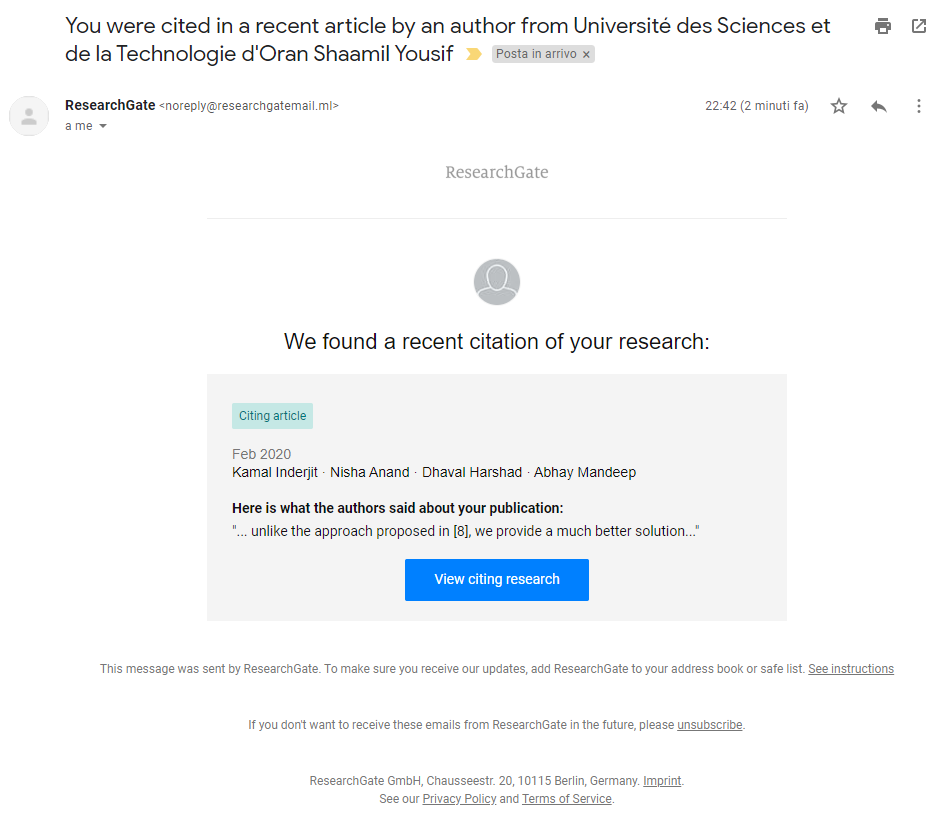
\includegraphics[scale=0.6]{images/templates/mir-doc-researchgate-citation.PNG}}
	\caption{Template "ResearchGate Citation" - Scenario 4}
	\label{template-s4b3}
\end{figure}

\newpage

\noindent
\textbf{Template "Risultati Employee Satisfaction".} This template, shown in Fig. \ref{template-s5b3}, was inspired by the annual email announcing the Employee Satisfaction Survey results. Linked to Scenario 5, it exclusively targeted technical and administrative staff. I felt that reading survey results would not be interesting enough. The "Enterprise Phishing Resiliency and Defense Report" by PhishMe, showed that safety and health are important topics to workers \cite{report-phishme}. Consequently, I specifically mentioned common issues like bathroom cleaning and office mold, as a additional stimulus.

\bigskip

\begin{figure}[H]
	\centering
	\fbox{
\includegraphics[scale=0.6]{images/templates/mir-pta-risultati-employee-satisfaction.PNG}}
	\caption{Template "Risultati Employee Satisfaction" - Scenario 5}
	\label{template-s5b3}
\end{figure}

\newpage

\subsection{Education}

\subsubsection{Landing Page}

The base landing page was cloned from the official website of the University of Padua \cite{website-unipd}. The final design of the landing page is shown in Fig. \ref{edu-landing}.

\begin{figure}[H]
	\centering
	\fbox{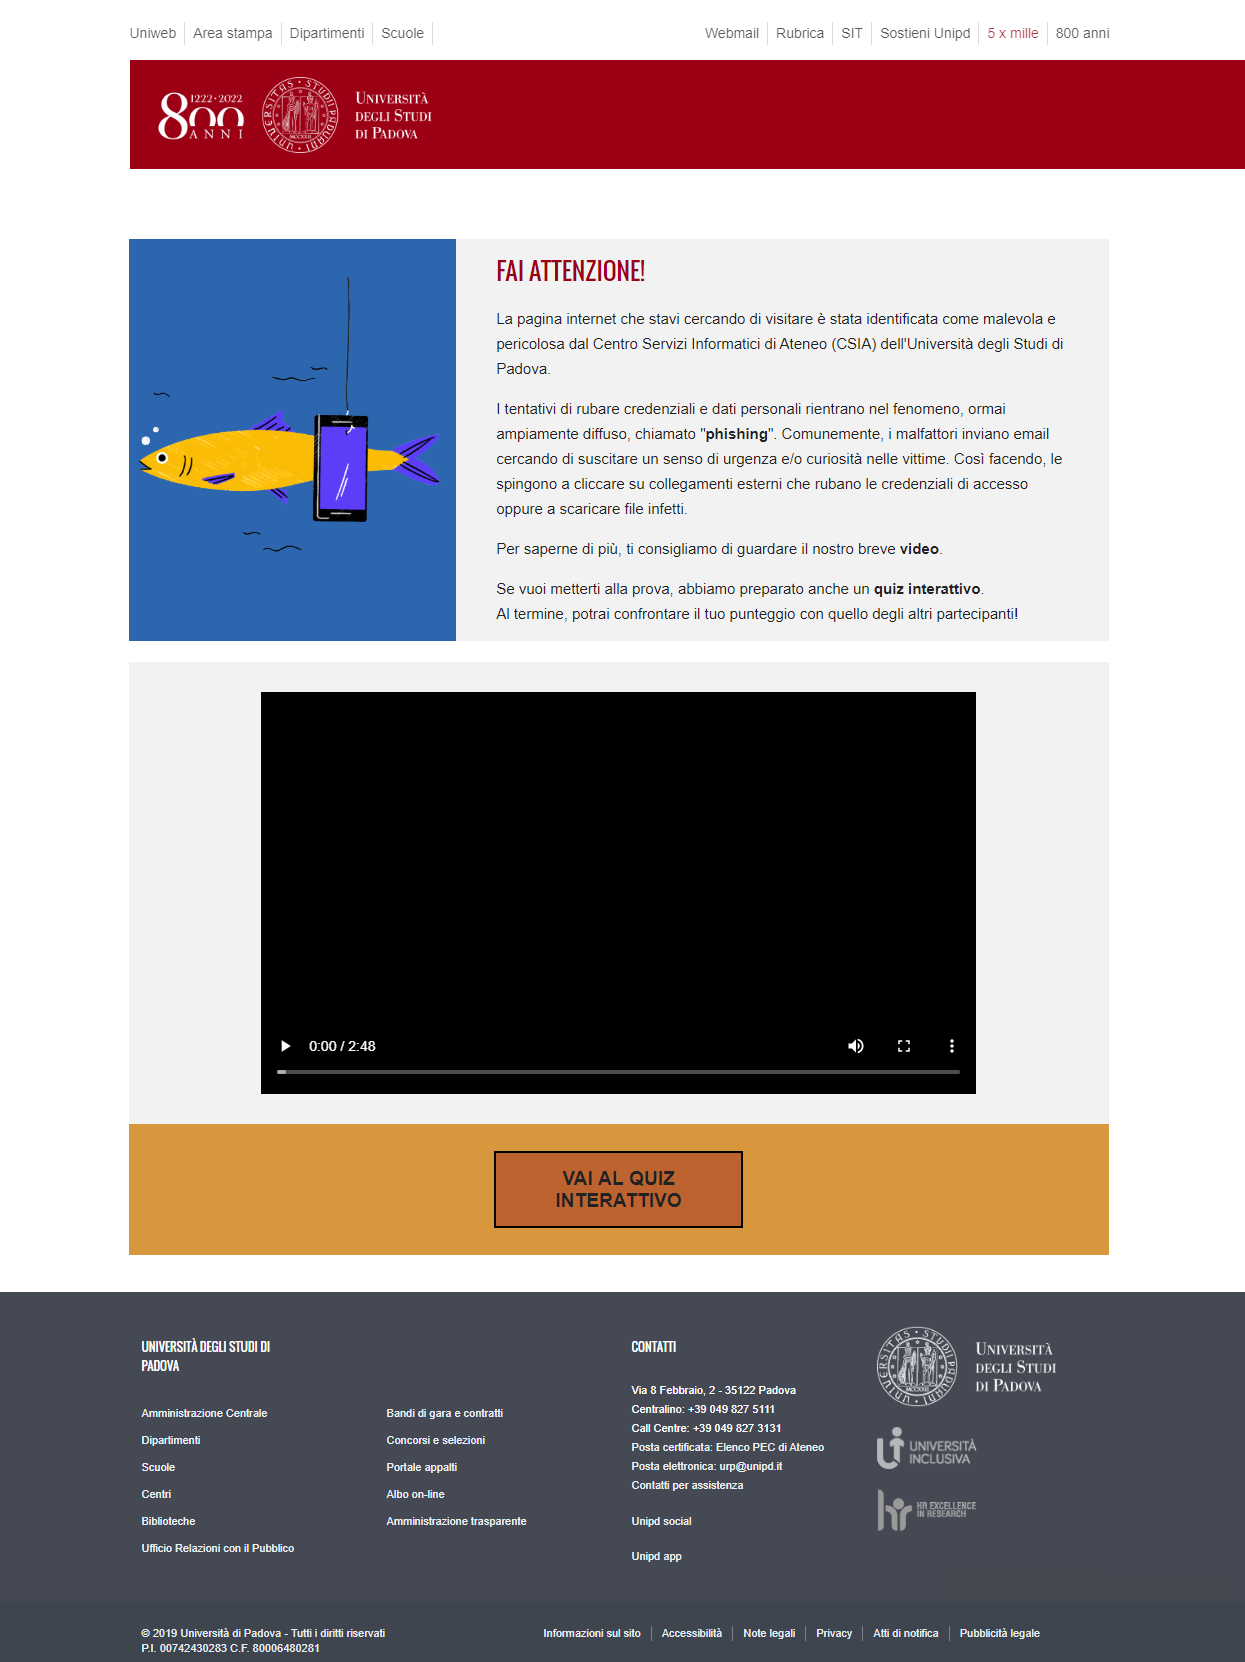
\includegraphics[scale=0.38]{images/education/landing.PNG}}
	\caption{Education - Landing Page}
	\label{edu-landing}
\end{figure}

\noindent
The landing page was my most important point of contact with subjects, so I focused on two core aspects: reassuring victims and explaining the concept of phishing.
\\ \\
\textbf{Reassuring victims.} This goal comes as a logical consequence of the discussion presented in the "Ethics" section of this thesis. Avoiding to bring harm to subjects was my first priority. In fact, the very first message on the landing page was dedicated to that matter. Upon looking at the familiar template and the legitimate domain in the URL address "@[phishing.]math.unipd.it", victims would likely avoid a panicking reaction. Without them being scared out of the landing page, they would have some chance to read the rest of the content.
\\ \\
The small paragraph in the landing page stated that the ICT Office detected a malicious URL and replaced it with that landing page, promoting phishing awareness. However, there was never a malicious URL and the email redirected to the landing page from the very beginning (as explained in previous sections). I capitalized on the shock value of the event, to make the victim feel that next time there could be real consequences.
\\ \\
\textbf{Explaining the concept of phishing.} After clarifying the situation in the first paragraph, I followed up with a basic explanation about the concept of phishing, encouraging victims to watch a short educational video and challenge themselves on an interactive quiz. I predicted that most victims would only read this short explanation, so I tried to make it as concise and useful as possible.

\subsubsection{Video}

\noindent
Nowadays, videos are a common medium for information, popular among people of all ages and skills. I figured that, as the first educational approach, a video would be the perfect fit for a difficult topic such as phishing prevention. For this task, I was supported by a lightboard. The lightboard is an innovative technology that allows to write on a surface while facing towards the audience. Using this technology I could talk face-to-face with subjects, as a basic form of debriefing process. A frame of the video is shown in Fig. \ref{edu-video}.

\begin{figure}[H]
	\centering
	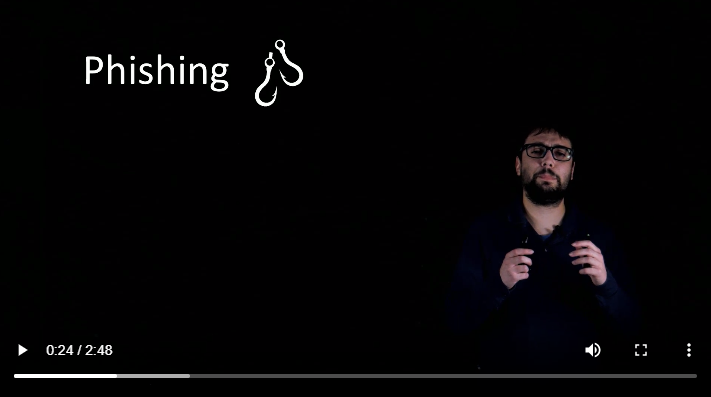
\includegraphics[width=\linewidth]{images/education/video.PNG}
	\caption{Education - Lightboard Video}
	\label{edu-video}
\end{figure}

\noindent
The video was designed to last a few minutes and to explain how to avoid phishing. The contents were the following:

\begin{itemize}
    \item a basic explanation and an email example;
    \item emotional motivators, specifically urgency and curiosity;
    \item website cloning and malicious attachments;
    \item defending ourselves by checking sender address, by checking URLs, and by dominating our initial instinct.
\end{itemize}

To track victim's watch time, I implemented a simple Javascript timer. The timer starts when pressing "Play", and pauses when pressing "Pause". As soon as two and a half minutes have passed (total length of 2:48), that specific individual would have its entry added on the education database.

\subsubsection{Quiz}

\noindent
For the second educational approach, I wanted to tackle more advanced and technical topics. To maximize the number of participants, I looked to design a fun learning experience and was inspired by Google's interactive phishing quiz \cite{tools-google-phishing-quiz}. I developed my own version, specifically tailored for the University of Padua. To foster a sense of curiosity on the victims, I actively challenged them to complete the quiz and promised them a chart with the results of all participants. My version of the quiz can be found at \url{https://quiz-unipd-phishing.herokuapp.com/?rid=thesis}.
\\ \\
The opening screen provided some background, assigned a random name and email to the participant and explained the basic rules. Afterwards, the quiz introduced one email at the time, asking to label it as "Legitimate" or "Phishing", as shown in Fig. \ref{edu-quiz-answer}.

\bigskip

\begin{figure}[H]
	\centering
	\fbox{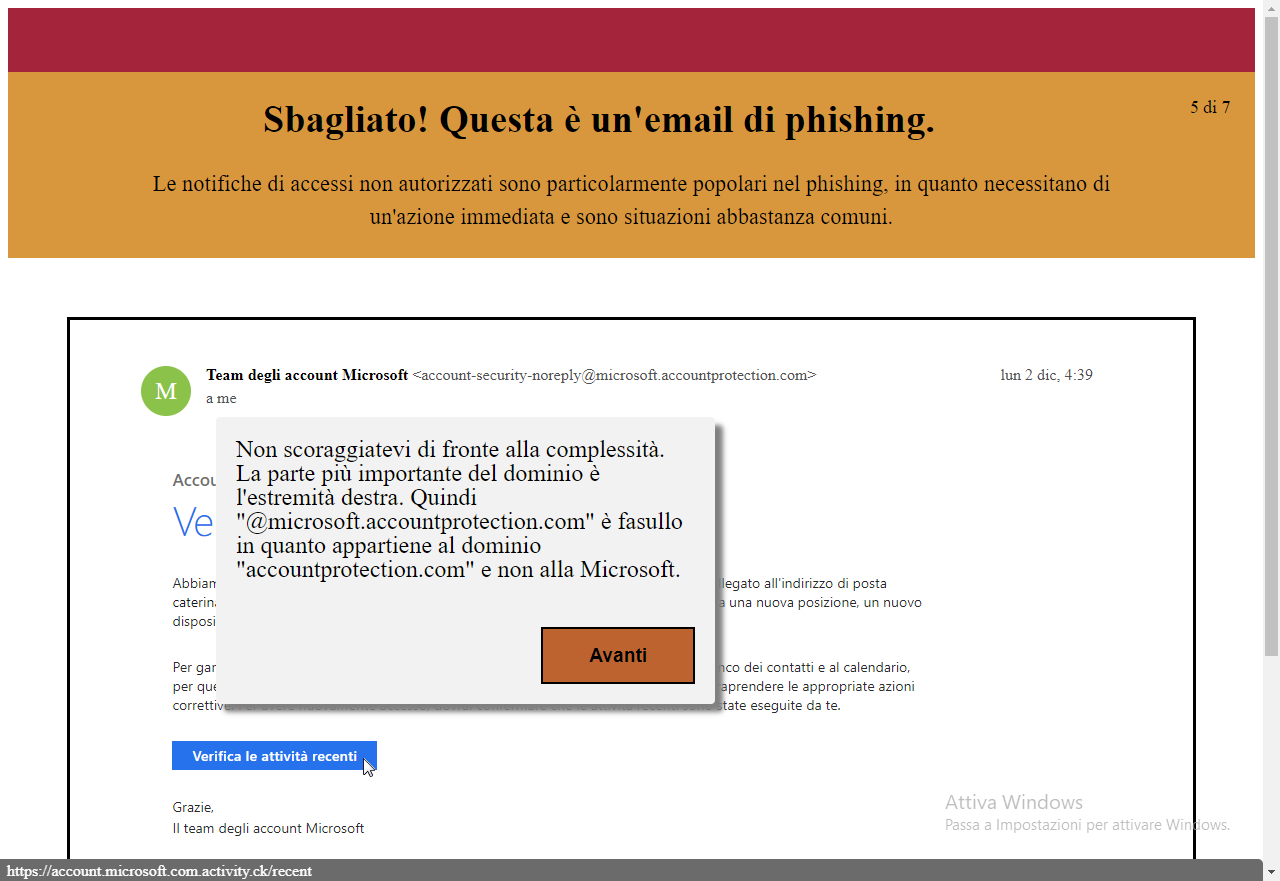
\includegraphics[width=\linewidth]{images/education/quiz-answer.PNG}}
	\caption{Education - Interactive Quiz - Answering}
	\label{edu-quiz-answer}
\end{figure}

\newpage

\noindent
After the answer, a short explanation was given and the quiz emphasized few important observations, carefully leading the user through the email content. The participants could freely check the sender address, the email content and the URLs. To better simulate a real environment, hovering over a link created the familiar visual bar at the bottom of the screen, showing the true destination of the link.
\\
The quiz spanned over seven emails, congratulating the participant at the end and displaying a chart with the aggregated score distributions from all the participants, as shown in Fig. \ref{edu-quiz-score}.

\bigskip

\begin{figure}[H]
	\centering
	\fbox{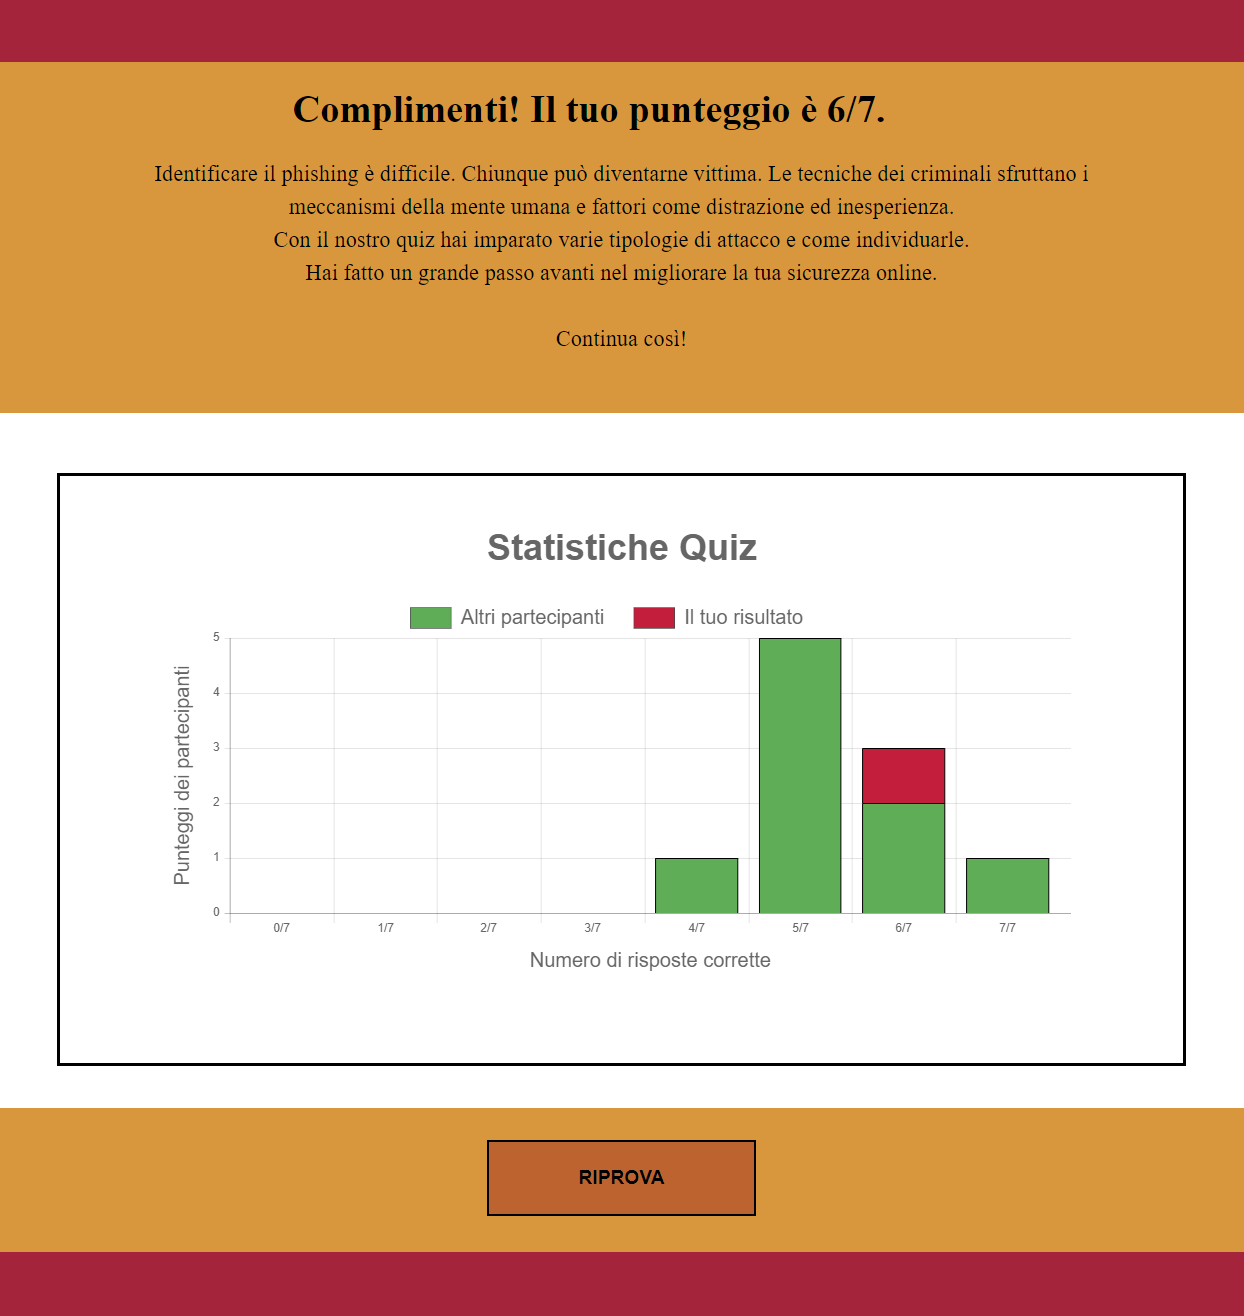
\includegraphics[width=\linewidth]{images/education/quiz-chart.PNG}}
	\caption{Education - Interactive Quiz - Score Distributions}
	\label{edu-quiz-score}
\end{figure}

\newpage

\subsection{Statistical Analysis}

\subsubsection{Chi-Squared Test}

One important goal of the phishing assessment was to review possible factors that contributed to phishing susceptibility. Therefore, I wanted to analyze the relationship between the Reaction and the other variables. The Chi-Squared Test for Independence tests if two categorical variables are related from a statistically significant point of view \cite{stats-chi-squared}. 
\\ \\
Benefits of the Chi-Squared Test for Independence were:

\begin{itemize}
    \item simple and intuitive;
    \item compatible with categorical variables (Age was considered as categorical);
    \item contingency table already available from Gophish' results;
    \item supports variables with more than two possible values (Age, Category, Subcategory, Scenario);
    \item outputs a statistical correlation between variables, fulfilling one of my goals.
\end{itemize}

Chi-Squared Test for Independence is a statistical hypothesis test. In each test, the null hypothesis was formulated as "Variable [Gender, Age, Category, Subcategory, Scenario] is independent from the Reaction variable, in the population related to the phishing assessment results". The input for the test was the contingency table with observed values from the whole experiment. The output of the test was a p-value: the probability to obtain results at least as extreme as the ones calculated in the test, assuming the validity of the null hypothesis. In other words, p-value is the chance that test results were arbitrary and not trustworthy. The standard significance level is represented by a p-value of "0.05".
\\ \\
If I consider two variables as independent from each other, but I obtain a low p-value (under the significance level), it means that the results obtained were incredibly unlikely. Unlikely to the point that those two variables are, in fact, correlated and not independent. Conversely, obtaining a high p-value (above the significance level) does not prove that those two variables are independent. Instead, it means that not enough statistically significant evidence was found.

\subsubsection{Binary Logistic Regression}

One important goal of the phishing assessment was to review possible factors that contribute to phishing susceptibility. Chi-Squared Test analyzes only variables in pairs. Instead, I wanted to evaluate the relationship between the predictors (Gender, Age, Category, Scenario) and the dependent variable (Reaction). Another important goal was to develop a predictive model trained by data gathered from the experiment. Binary Logistic Regression creates a predictive model, taking into account all the variables at the same time \cite{stats-binary-logistic-regression}. 
\\ \\
Benefits of the Binary Logistic Regression were:

\begin{itemize}
    \item multivariate and descriptive;
    \item compatible with categorical variables (Age was considered as categorical);
    \item compatible with a binary dependent variable (Reaction had a binary outcome);
    \item contingency table already available from Gophish' results;
    \item supports predictors with more than two possible values (Age, Category, Scenario);
    \item outputs a statistical correlation between variables, fulfilling one of my goals;
    \item outputs a predictive model, fulfilling one of my goals.
\end{itemize}

\noindent
Binary Logistic Regression yields a complex table as its output \cite{stats-interpretation-blr}. Rows represent predictors while columns represent statistical data. 
\\ \\
\textbf{Rows.} Each row corresponds to a possible value of a predictor (Intercept is a special case). For example, the predictor Scenario has four different possible values: S2, S3, S4, S5. As a reminder, a "possible value of a predictor" is just another way to spell "a trait". Each row of the table corresponds to a trait.
\\
The first trait of each predictor is absent from the table because it acts as a reference point. Categorical predictor coefficients are formulated "w.r.t." (with respect to) other traits of the same predictor. More details can be found in the "Estimate" paragraph below.
\\ \\
\textbf{Estimate.} The "Estimate coefficient" describes the influence of a predictor's value with respect to the baseline trait (the missing one). A row with a positive Estimate coefficient means that an individual with that row's trait is more susceptible to phishing. Conversely, a negative Estimate indicates a lower susceptibility. A predictor's baseline value is simply considered as 0.
\\
Comparing two Estimate coefficients may give additional insight. A trait with double the coefficient of a another trait, has double the influence on phishing susceptibility (compared to that other trait). However, the Estimate coefficient is not a direct measure of the magnitude of effect of a predictor.  
\\ \\
\textbf{Intercept.} The "Intercept", also called "Constant", is a complex element. In my case, I just need it to develop predictions from the Estimates, through the formula known as logistic transformation. More details can be found in the "Prediction" paragraph.
\\ \\
\textbf{Standard Error.} The "Standard Error" is used to determine how well a model fits the data, and to assess the precision of predictions.
\\ \\
\textbf{z-value.} The "z-value" is obtained by dividing the Estimate coefficient for the Standard Error. Significant traits are identified by a z-value of higher magnitude.
\\ \\
\textbf{Pr(\textgreater z).} The "Pr(\textgreater z)" value has the same role as the p-value in Chi-Squared Test. As a reminder: it describes the likelihood to get the same result calculated in the test, but under the (hopefully unreasonable) null hypothesis. The null hypothesis would be "the predictor is independent from the dependent variable (Reaction)". It is not a direct measure of the magnitude of effect of a predictor. 
\\
"Pr(\textgreater z)" is compared to the five significance levels in the legend and discussed in the "Significance Codes" paragraph below. A lower "Pr(\textgreater z)" corresponds to a more significant trait.
\\ \\ \\
\textbf{Significance Codes.} The "Significance Codes" are intuitive visual cues about the significance of a trait. A legend explains which symbols correspond to which range of values. Significance Codes are applied to the value of the "Pr(\textgreater z)" column for each row.
\\ \\
\textbf{AIC.} The "Aikake Information Criterion" is a common estimator for the quality of a predictive model. It mediates between the goodness of fit and the simplicity of the model. Models with lower AIC are preferable. The "Number of Fisher Scoring iterations" is related to how the model fit was estimated. Logistic Regression requires an iterative approach to evaluate model fitness, and the amount of iteration performed is exactly the "Number of Fisher Scoring iterations".

\newpage

\subsection{Software and Tools}

\subsubsection{Gophish}

Gophish is an open-source phishing framework \cite{tools-gophish}. It manages most aspects of a phishing campaign and requires minimal setup. Installing Gophish as a service on the virtual machine over SSL was simple enough. A critical part was taking care of user permission and configuring the settings within Unipd network infrastructure.
\\ \\
Gophish was a core component of the project and its features will be discussed in depth, following the structure of Gophish' graphical interface tabs.
\\ \\
\textbf{Email Templates.} Email templates are the key elements in a phishing campaign. Templates can be easily created and appear on a list, that can be modified at any time. Gophish' email templates tab is shown in Fig. \ref{gop-ttab}.

\begin{figure}[H]
	\centering
	\fbox{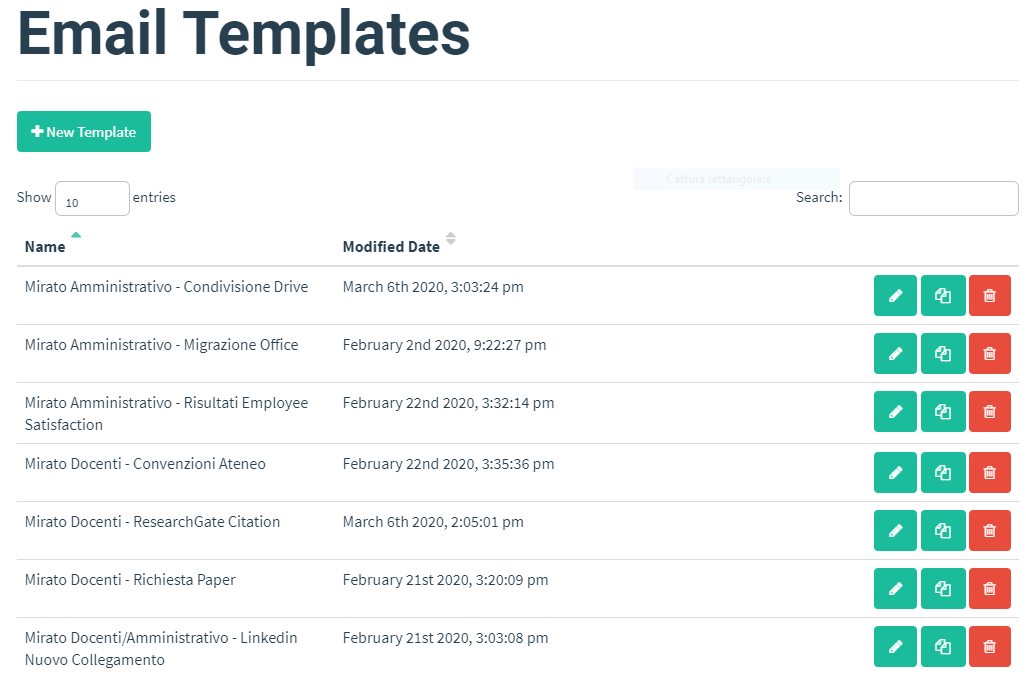
\includegraphics[scale=0.4]{images/tools/gophish-templates-menu.PNG}}
	\caption{Gophish - Email Templates Tab}
	\label{gop-ttab}
\end{figure}

\noindent
Gophish allows to directly import and clone emails, or to design one on your own. Templates could be composed in plaintext or HTML. To better automate customization, several variables are available to the HTML format:

\begin{itemize}
    \item {{.RId}}, the target's unique ID;
    \item {{.FirstName}} and {{.LastName}}, the target's first and last name;
    \item {{.Email}}, the target email address;
    \item {{.Tracker}}, the tracking image;
    \item {{.URL}}, the phishing URL.
\end{itemize}


Given the privacy constraints, I was severely limited in their usage. Personal data about subjects was out of reach, and the email were just aliases. Still, I used {{.URL}}, the recommended way to craft the phishing URL and {{.Tracker}}, to enable tracking functionalities. The creation of a new template on Gophish is shown in Fig. \ref{gop-tnt}.

\begin{figure}[H]
	\centering
	\fbox{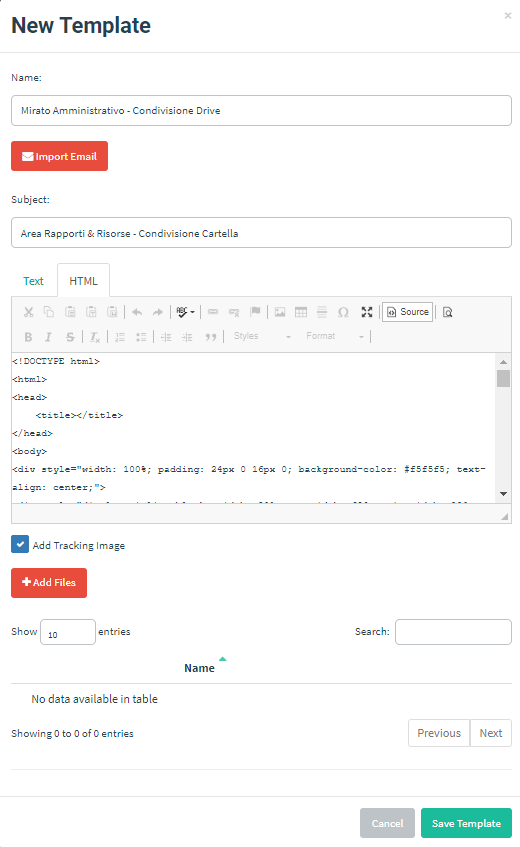
\includegraphics[scale=0.58]{images/tools/gophish-templates-sample.PNG}}
	\caption{Gophish - Email Templates - New Template}
	\label{gop-tnt}
\end{figure}

\noindent
\textbf{Sending Profiles.} In every Gophish campaign the sender profile has to be specified. Sending profiles can be freely created and appear on a list, that can be modified at any time. Gophish' sending profiles tab is shown in Fig. \ref{gop-sp}.

\begin{figure}[H]
	\centering
	\fbox{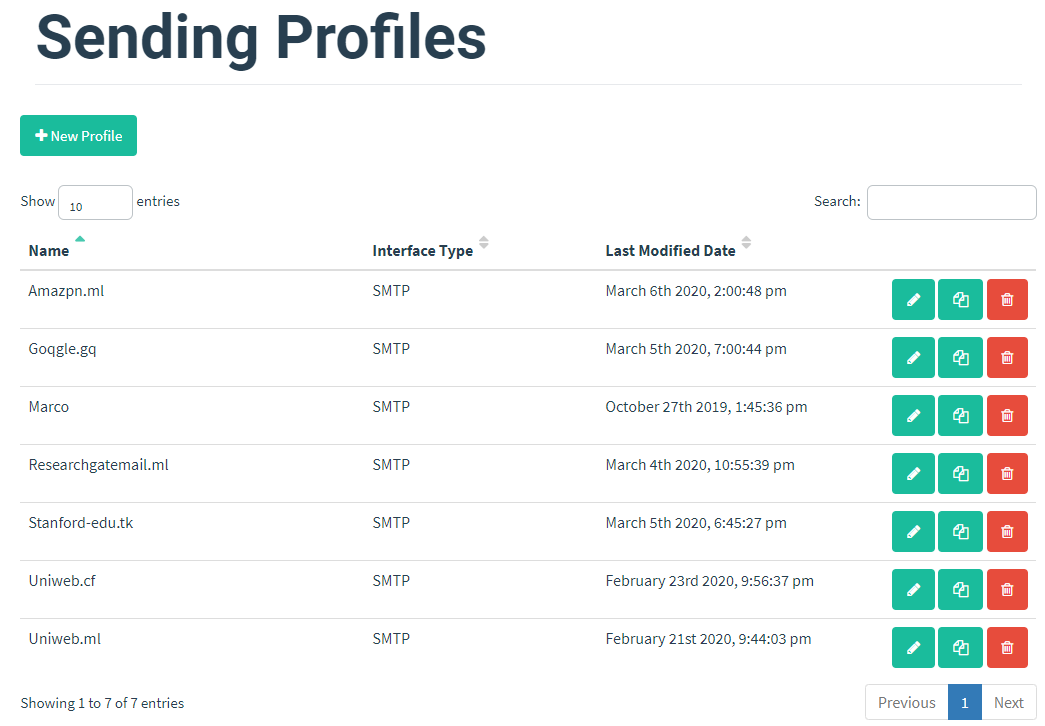
\includegraphics[scale=0.38]{images/tools/gophish-sending-menu.PNG}}
	\caption{Gophish - Sending Profiles}
	\label{gop-sp}
\end{figure}

\noindent
A sending profiles needs a sender domain, as the FROM header, and information about the SMTP server (hostname, username and password). The domains I utilized were registered by me on Freenom \cite{tools-freenom}, and I compiled the SMTP server information field with parameters from SendGrid  \cite{tools-sendgrid}. Header spoofing was available but was not needed for the experiment. The creation of a new sending profile on Gophish is shown in Fig. \ref{gop-spnsp}.

\begin{figure}[H]
	\centering
	\fbox{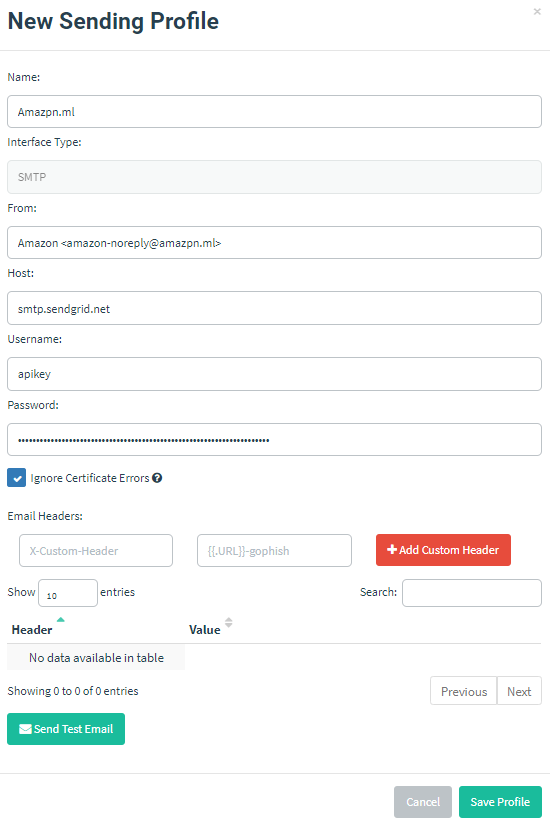
\includegraphics[scale=0.53]{images/tools/gophish-sending-sample.PNG}}
	\caption{Gophish - Sending Profiles - New Sending Profile}
	\label{gop-spnsp}
\end{figure}

\noindent
\textbf{User \& Groups.} In every Gophish campaign targets have to be specified. Targets are defined by groups, where multiple email addresses can be added as a new targeted user group. Groups can be freely created and appear on a list, that can be modified at any time. Gophish' user \& groups tab is shown in Fig. \ref{gop-ug}.

\begin{figure}[H]
	\centering
	\fbox{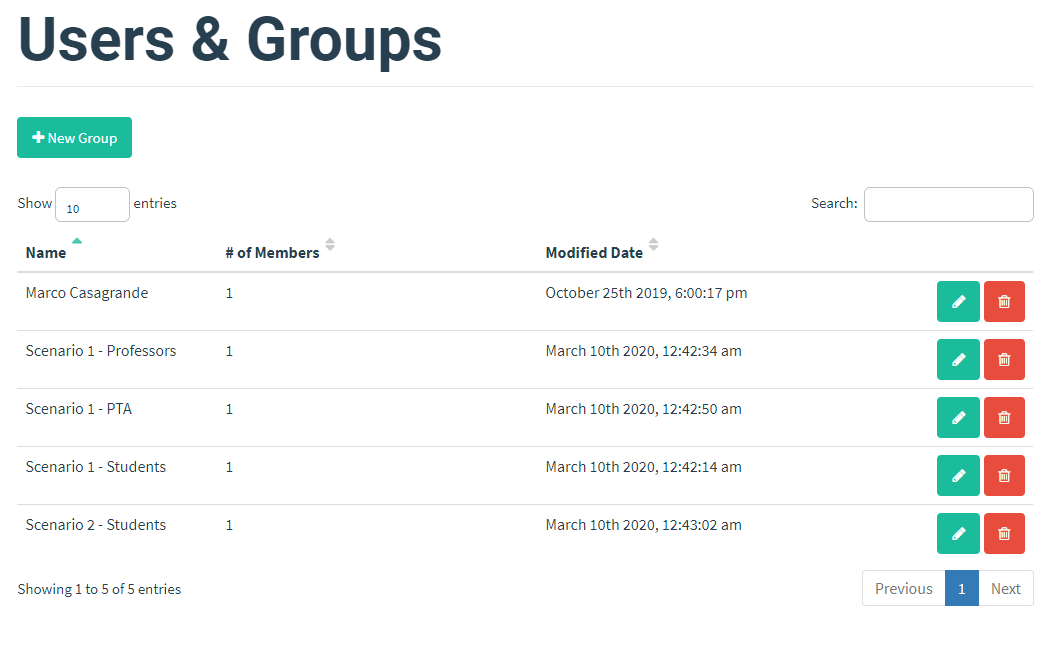
\includegraphics[scale=0.36]{images/tools/gophish-groups-menu.PNG}}
	\caption{Gophish - User \& Groups}
	\label{gop-ug}
\end{figure}

\noindent
For the groups, I simply imported the targets in bulk from a CSV file, obtained by parsing the my dataset. Each scenario would have a different group as its target. The creation of a new group of users on Gophish is shown in Fig. \ref{gop-ugng}.

\begin{figure}[H]
	\centering
	\fbox{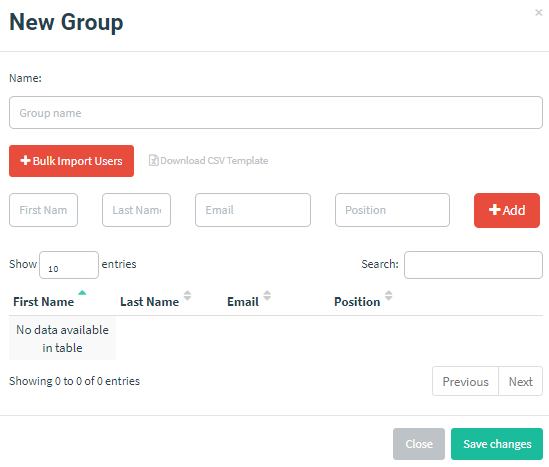
\includegraphics[scale=0.38]{images/tools/gophish-groups-sample.PNG}}
	\caption{Gophish - User \& Groups - New Group}
	\label{gop-ugng}
\end{figure}

\noindent
\textbf{Landing Pages.} Landing pages are the final destination of any phishing URL crafted by Gophish. Landing pages can be freely created and appear on a list, that can be modified at any time. In my case, I only needed a single landing page, as every subject would be offered the same one, with the same educational content. Gophish' landing pages tab is shown in Fig. \ref{gop-lp}.

\begin{figure}[H]
	\centering
	\fbox{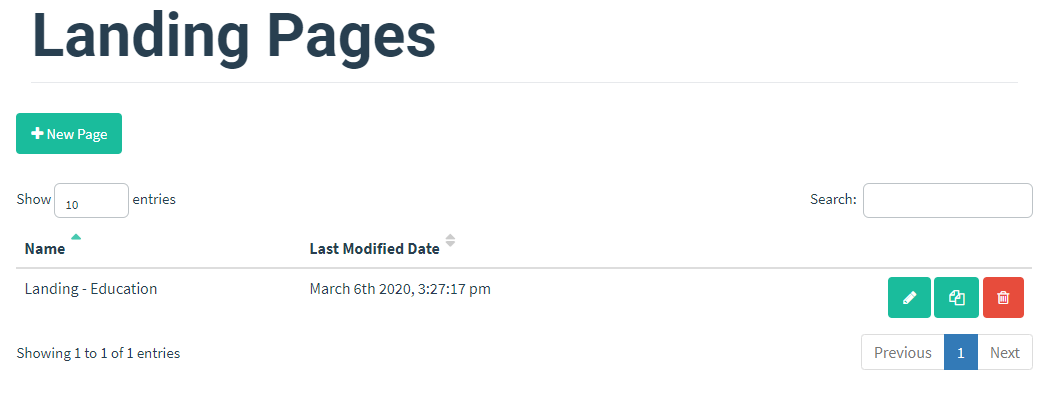
\includegraphics[scale=0.28]{images/tools/gophish-landings-menu.PNG}}
	\caption{Gophish - Landing Pages}
	\label{gop-lp}
\end{figure}

\noindent
The landing page was written in HTML, embedding CSS and Javascript tags. The core page was imported from a real page on Unipd website, and then repurposed for my own goals. Landing page setting allow the collection of data submitted by users through forms. I did not ask for any personal information, so that functionality was turned off. The creation of a new landing page on Gophish is shown in Fig. \ref{gop-lpnlp}.

\begin{figure}[H]
	\centering
	\fbox{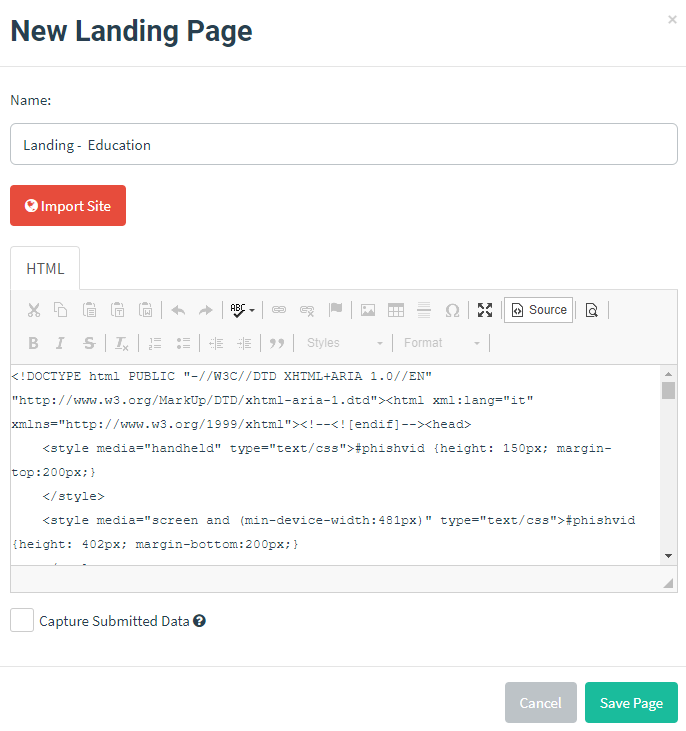
\includegraphics[scale=0.35]{images/tools/gophish-landings-sample.PNG}}
	\caption{Gophish - Landing Pages - New Landing Page}
	\label{gop-lpnlp}
\end{figure}

\noindent
\textbf{Campaign.} The creation of a new phishing campaign is the final step in the process. Each campaign appears on a list, and its progress can be reviewed at any time. Gophish' campaigns tab is shown in Fig. \ref{gop-cpgn}.

\begin{figure}[H]
	\centering
	\fbox{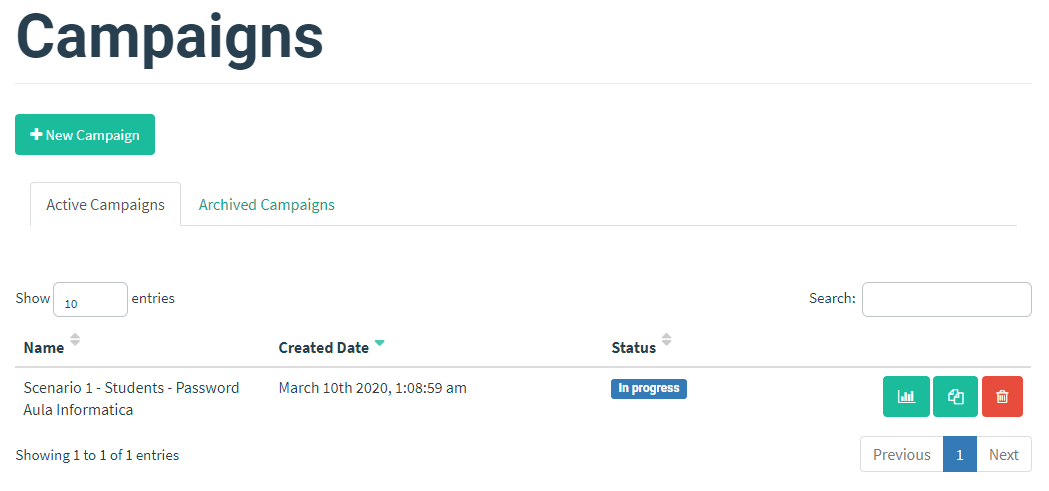
\includegraphics[scale=0.3]{images/tools/gophish-campaign-menu.PNG}}
	\caption{Gophish - Campaigns}
	\label{gop-cpgn}
\end{figure}

\noindent
To create a Gophish campaign, one must choose from the various elements created on the previous four tabs: "Email Templates", "Landing Pages", "Sending Profiles" and "Users \& Groups". Additionally, settings related to timed email delivery are available. The creation of a new campaign on Gophish is shown in Fig. \ref{gop-cpgnnc}.

\begin{figure}[H]
	\centering
	\fbox{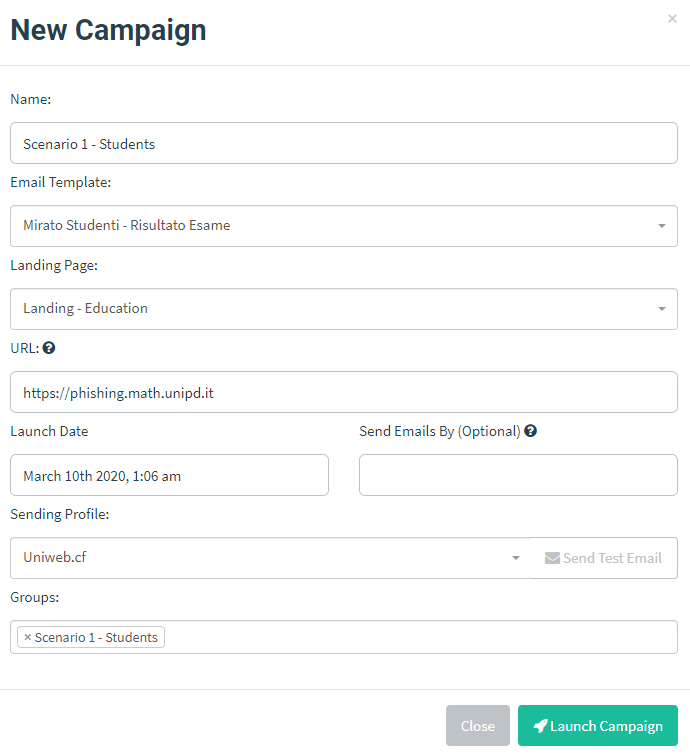
\includegraphics[scale=0.45]{images/tools/gophish-campaign-sample.PNG}}
	\caption{Gophish - Campaigns - New Campaign}
	\label{gop-cpgnnc}
\end{figure}

\noindent
When creating a new campaign, the most important field is the "URL", the location of Gophish' listener. This URL becomes the base for every other Gophish phishing URL, specified as {{.URL}} inside the templates. To the base URL, Gophish attaches (as a parameter) an unique identifier, the {{.RId}}, attributed to the specific targeted user. Only addresses with those {{.RId}} parameters are actually created and can be accessed by users. Since my base URL was \textit{https://phishing.math.unipd.it/}, I asked the IT Support in the Department of Mathematics to allow external connections. Thanks to Certbot \cite{tools-certbot}, I could then provide a secure connection instead of the default HTTP one.

\newpage

\noindent
Gophish has an overview page dedicated to displaying statistics of each specific campaign, as shown in Fig. \ref{gop-cco}. Three three incredibly useful elements can be looked at:

\begin{itemize}
    \item Campaign Timeline - showing every event occurred throughout the campaign's duration;
    \item Campaign Statistics - showing the number of emails which exhausted each of the five types of event;
    \item Campaign Details - showing much greater details about each and every target.
\end{itemize}

\begin{figure}[H]
	\centering
	\fbox{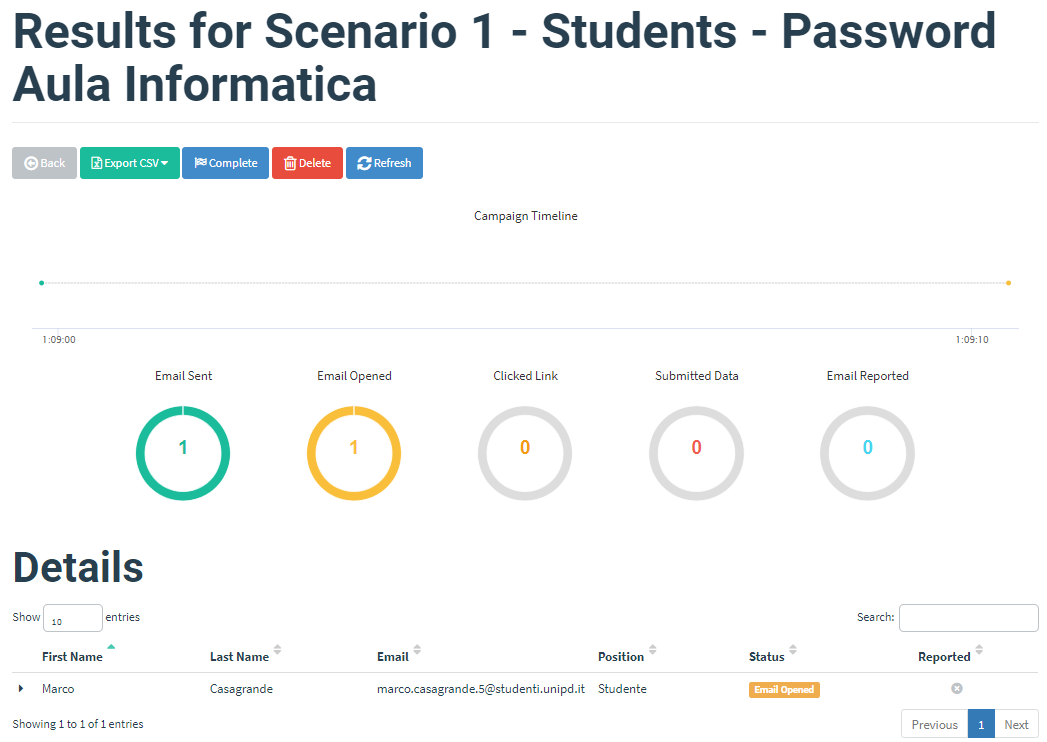
\includegraphics[scale=0.45]{images/tools/gophish-campaign-overview.PNG}}
	\caption{Gophish - Campaigns - Campaign Overview}
	\label{gop-cco}
\end{figure}

\noindent
Since I didn't want to capture submitted data, nor I had any report functionality to test, the statistics I would be using were the first three: "Sent", "Opened", and "Clicked".
\\ \\
A complete review of the campaign events and results can be found in a CSV file.

\subsubsection{Ngrok}

Ngrok is a service used to expose local servers to the public, through secure tunnels \cite{tools-ngrok}. Since Gophish needed a graphical interface to be operated, navigating through shell commands was impractical. Using Ngrok, I always worked using a secure tunnel to Gophish' server interface. Ngrok tunneling through shell commands is shown in Fig. \ref{ngrok-tunnel}.

\begin{figure}[H]
	\centering
	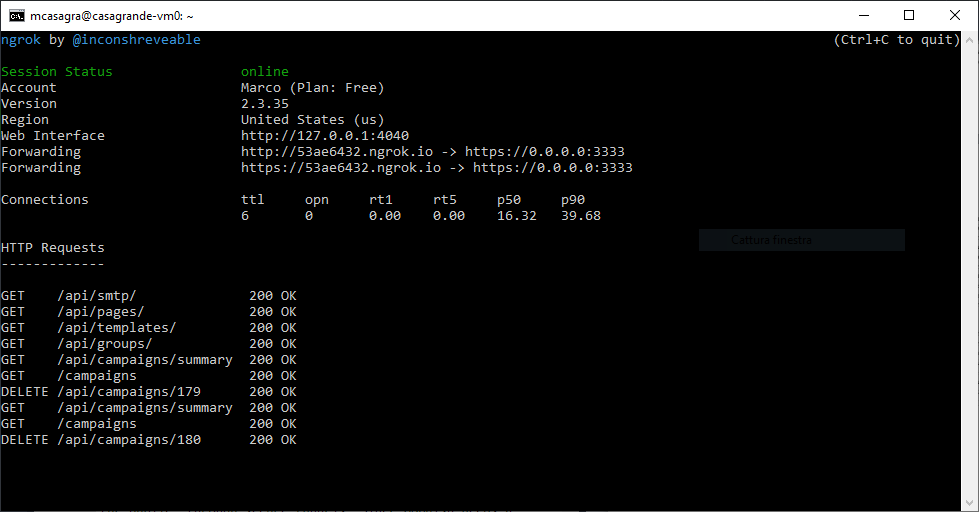
\includegraphics[scale=0.35]{images/tools/ngrok-tunnel.PNG}
	\caption{Ngrok Tunnel}
	\label{ngrok-tunnel}
\end{figure}

\subsubsection{SendGrid}

SendGrid is a cloud-based SMTP provider that acts as an email delivery engine \cite{tools-sendgrid}. The service's core purpose is the creation, management and tracking of promotional and commercial email campaigns. In my case, I needed it mostly as a SMTP provider. Every other aspect of the phishing simulation was already taken care by Gophish. 
\\ \\
One vital privacy constraint was to not receive any responding message from the subjects, automated or not. SendGrid simply delivers emails from a domain to the targets, without receiving any response, thus satisfying the constraint.
\\ \\
In order to send emails from within Unipd network, Sendgrid's SMTP server was whitelisted by IT Support.
\\ \\
While using Sendgrid, link tracking was innately on. Since any SendGrid link appeared as "suspicious" in Gmail, I absolutely needed to turn it off. Even after switching it off, link tracking was still enabled. I had to manually disable the feature by writing "<a clicktracking=off></a>" on every anchor tag of each template,.

\subsubsection{Freenom}

Freenom is a free Internet Domain provider \cite{tools-freenom}. Several custom domains are needed as the phishing email senders. Freenom provides five free Internet country code top-level domains (".tk", ".ml", ".ga", ".cf", ".gq"), coupled with any name of choice, if not already taken.
\\ \\
Even though I did want to succeed in phishing people, I also needed to give them a fair chance to spot the fraud. So I relied on those free domains, instead of spoofing an email address or sending them from a real Unipd account. My domains looked similar to their real counterparts, but were still fairly recognizable as fakes:

\begin{itemize}
    \item "@uniweb-unipd.cf", mimicking Uniweb;
    \item "@amministr-uniweb.ml", mimicking Uniweb;
    \item "@unipd.ga", mimicking Unipd;
    \item "@amazpn.ml", mimicking Amazon;
    \item "@goqgle.gq", mimicking Google;
    \item "@researchgatemail.ml", mimicking the social network ResearchGate;
    \item "@stanford-edu.tk", mimicking a Stanford University professor.
\end{itemize}

To remove any mention of Sendgrid in the sender address, I needed to authenticate my domains. By adding some CNAME records to the domain, as shown in Fig. \ref{freenom-dns}, SendGrid confirmed my ownership and the authentication process was complete. Otherwise, without that adjustment, the sender would, for example, appear as "Amministrazione Uniweb <amministrazione.uniweb@uniweb-unipd.ml> sent via SendGrid".

\begin{figure}[H]
	\centering
	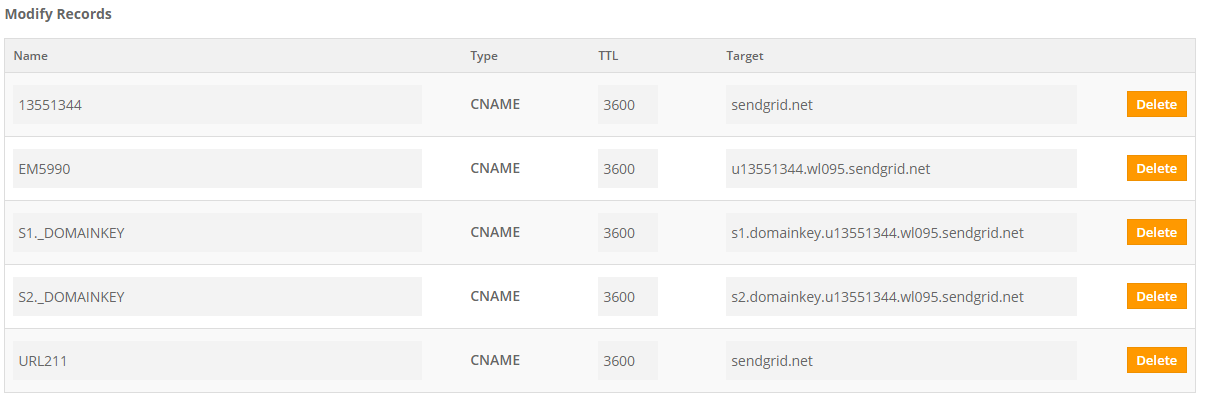
\includegraphics[scale=0.32]{images/tools/freenom-dns.PNG}
	\caption{SendGrid's brand authentication by adding domain DNS records}
	\label{freenom-dns}
\end{figure}

\noindent
Since I used the same SendGrid account for every domain, I needed to create one API key for each domain. Those were inputted in the "Sending Profiles" page for each sender domain.

\newpage

\subsubsection{Heroku}

Heroku is a cloud platform that lets companies build, deliver, monitor and scale apps \cite{tools-heroku}. In my project, Heroku was used for a few purposes: 

\begin{itemize}
    \item Interactive Phishing Quiz, to supply educational content to the landing page;
    \item Tracking Pixels Loggers, to manage information about custom tracking pixels;
    \item Phishing Database, to log my custom tracking pixels and educational-related data (quiz/video).
\end{itemize}

\noindent
\textbf{Interactive Phishing Quiz.} The interactive phishing quiz is part of the educational efforts \cite{tools-unipd-phishing-quiz}. It is a straightforward web app, written in HTML, PHP and Javascript. On completing the quiz, an education entry for the participant is sent to a database and the combined results of every other participant are displayed.
\\ \\
\textbf{Tracking Pixels Loggers.} The web app consists of a few lines of code. Any tracking pixel loads an image from \textit{https://frozen-wildwood-51801.herokuapp.com/event\_name.php/?rid=value} that logs into the database the event ("opened", "clicked"), the timestamp and the RId of the user. Those tracking pixel were used to assess the reliability of Gophish' ones.
\\ \\
\textbf{Phishing Database.} The database is composed by four tables. The table "tracking", show in Fig. \ref{heroku-tracking}, stores events triggered by my own tracking pixels. The table "eduv", show in Fig. \ref{heroku-eduv}, stores entries related to watching the educational video. The table "eduq", show in Fig. \ref{heroku-eduq}, stores entries related to completing the educational quiz. The table "quiz", show in Fig. \ref{heroku-quiz}, stores the overall quiz scores, shown as a chart at the end of the quiz itself.

\bigskip

\begin{figure}[H]
	\centering
	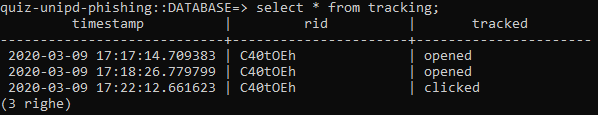
\includegraphics[scale=0.6]{images/tools/database-tracking.PNG}
	\caption{Database Table "tracking"}
	\label{heroku-tracking}
\end{figure}

\begin{figure}[H]
	\centering
	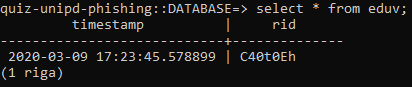
\includegraphics[scale=0.7]{images/tools/database-eduv.PNG}
	\caption{Database Table "eduv"}
	\label{heroku-eduv}
\end{figure}

\begin{figure}[H]
	\centering
	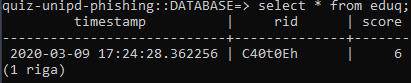
\includegraphics[scale=0.7]{images/tools/database-eduq.PNG}
	\caption{Database Table "eduq"}
	\label{heroku-eduq}
\end{figure}

\begin{figure}[H]
	\centering
	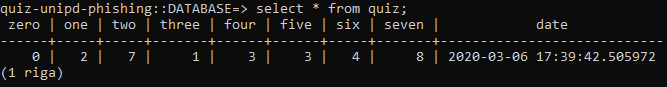
\includegraphics[scale=0.5]{images/tools/database-quiz.PNG}
	\caption{Database Table "quiz"}
	\label{heroku-quiz}
\end{figure}

\subsubsection{Virtual Machine}

Since I highly valued security, I asked to host Gophish on a machine inside Unipd network. The virtual machine ran Gophish as a service and was given free access to the address "phishing.math.unipd.it", to be used for the landing page. 
\\ \\
The address was granted a HTTPS connection by Certbot \cite{tools-certbot}, an open source software tool for automatically using Let’s Encrypt certificates on manually-administrated websites to enable HTTPS. SendGrid's SMTP server access to Unipd network was whitelisted so I could use it from the virtual machine without any issue.

\subsection{Avoiding Phishing Countermeasures}

\subsubsection{Gmail}

Student email accounts (ending with "@studenti.unipd.it") are autonomously managed by Gmail, even though emails still have to go through Unipd mail servers. 
\\ \\
Gmail was very adept in detecting malicious URLs that redirected to the educational landing page. Direct links to the landing page (\textit{https://phishing.math.unipd.it}) were completely fine. Adding any in-between redirection caused Gmail to issue a "suspicious website" warning. Using Gophish' machine IP address instead, caused my sender domain to get relegated into two prominent phishing blacklists: "Sorbs Spam" and "Lashback".

\subsubsection{Greylisting}

Mail servers at the University implement "greylisting": a defensive technique against spam. Any message from an unknown sender is temporarily rejected by the receiving email server. If the email is received a second time, after the rejection, it is accepted. Often enough, mass email spammers do not indulge in further attempts nor use queues; so a greylist effectively blocks them. Instead, a legitimate sender will reattempt to deliver the message and pass through greylisting.
\\ \\
Due to this technique, email delivery during the simulation could get delayed for a few hours. Greylisting was implemented separately on each mail server, so a single email could get rejected multiple times if each time it connected to a different server. This behaviour was not particularly problematic, but had to be accounted for when scheduling the attacks.

\subsubsection{Traffic Limit}

During the First Batch of phishing emails, I discovered some limitations to the amount of traffic I was allowed send before spam filter blocked me for spamming. If sent them all at the same time, even as few as twenty emails could get detected and blocked. Whenever that happened, the domain would be permanently listed on Spamhaus Zero Reputation Domains service \cite{website-spamhaus}. Ultimately, I set my traffic to about a hundred emails every few hours and did not incur in further issues.

\subsubsection{Tracking Email Openings}

Gophish, through its tracking pixel, can automatically track "Sent", "Opened" and "Clicked" events. Unfortunately, "Opened" events were triggering seemingly at random. I figured that Google Image Proxy (logged as "via ggpht.com GoogleImageProxy") was the culprit, but the issue was only partially solved. "Opened" events were still firing between zero and two times, before even reaching the victim. Sometimes, "Opened" events triggered after "Clicked" ones, or never.
\\ \\
From the available data, I could not find a logical pattern and I had to dismiss any analysis of "Opened" events, since they were proven to be unreliable. Still, that metric was not fundamental and I simply proceeded to ignore it during the analysis process.

\newpage

\section{Results and Discussion}
%% RESULT AND DISCUSSION

\subsection{Raw Results}

\subsubsection{Grand Total}

Raw results were extrapolated from the First Batch of phishing emails. Scenarios and Templates involved are the following:

\begin{itemize}
    \item Scenario 2 -> \hyperlink{template-s2b1}{Template "standard-google-avviso-sicurezza"};
    \item Scenario 3 -> \hyperlink{template-s3b1}{Template "mir-stud-risultato-esame"};
    \item Scenario 4 -> \hyperlink{template-s4b1}{Template "mir-doc-richiesta-paper"};
    \item Scenario 5 -> \hyperlink{template-s5b1}{Template "mir-pta-condivisione-drive"}.
\end{itemize}

\noindent
The data source for the following observations can be found in \hyperlink{appendix-results}{"Appendix B"}; in Table \ref{t-varreact0-grandtotal}, Table \ref{t-varreact0-scen} and Table \ref{t-varreact0-cat}.
\\ \\
\textbf{Overview.} Out of 1016 total emails delivered, a sizeable 31\% of them was clicked. The results were collected between the 12th and the 19th of March, two days after the last phish was delivered. The clickrate was similar to other case studies, although higher than expected. The sample size was comparatively larger so raw results should be fairly representative of the current situation at Unipd.
\\ \\
\textbf{Scenarios.} The four scenarios tested do show consistent results, proving that email templates were equal in difficulty. Scenario 2 was the worst performing one, since it lacked any customization. Still, it was not that far from targeted attacks' performance. 
\\ \\
\textbf{Categories.} A remarkable difference in percentage is shown when confronting employees (professors, technical and administrative staff) to students. A reasonable outcome, considering that students perceive their email account as less valuable than workers.

\subsubsection{Variable/Reaction Correlation}

Looking at the raw results from the simulation was useful in preparation to subsequent, more elaborated analysis. It gave me a panoramic about the whole study, and helped me in scouting for possible relationship between variables. 
\\ \\
I organized the raw results in a more readable format, aiming to find correlations between my independent variables (Gender, Age, Category) and my dependent variable (Reaction). I gave a crude interpretation of the data for each different Scenario.
\\ \\
Data sources for the following observations are mentioned at the end of each paragraph, and can be found in \hyperlink{appendix-varreact}{"Appendix B"}.
\\ \\
\textbf{All Scenarios.} Gender shows no particular behaviour. The most susceptible Age ranges clearly are the younger ones ("0-20" and "21-26"). At the same time, the least susceptible are the eldest ("61-99"). Apart from the second least susceptible ("36-40"), remaining Age ranges are fairly balanced. Observations about Category are the same as the ones presented in the "Grand Total" section above.
\\ \\
Table \ref{t-varreact1} shows the Variable/Reaction Correlation for All Scenarios. It can be found in \hyperlink{appendix-varreact}{"Appendix B"}.
\\ \\
\textbf{Scenario 2.} Phishing susceptibility swings wildly in relation to Age. The vast majority of students belong to the younger Age ranges ("0-20", "21-25" and "26-30"), which are, at the same time, the most susceptible ones. Student Category inflates the clickrate of Scenario 2, while the other two contenders display substantially lower percentages.
\\ \\
Table \ref{t-varreact2} shows the Variable/Reaction Correlation for Scenario 2. It can be found in \hyperlink{appendix-varreact}{"Appendix B"}.
\\ \\
\textbf{Scenario 3.} Scenario 3 specifically targets students, and the median Age reflects it. Younger students still are the most susceptible. Elder ones perform somewhat better, but the sample size is relatively small. Overall, students performed slightly better in Scenario 3 than in Scenario 2. Two main factors influenced this peculiar situation. First, student don't react immediately to phishing. Scenario 2 started a few days before Scenario 3, so more the former had more subjects that actively looked at emails. Second, students seem to care less about email content. As a consequence, targeted attacks are as effective as generic ones.
\\ \\
Table \ref{t-varreact3} shows the Variable/Reaction Correlation for Scenario 3. It can be found in \hyperlink{appendix-varreact}{"Appendix B"}.
\\ \\
\textbf{Scenario 4.} A peak in susceptibility is located around Age "46-50". The targeted attack was far more effective than the generic one (32\% vs 13\%). A valuable proof that spearphishing is a serious threat to employees.
\\ \\
Table \ref{t-varreact4} shows the Variable/Reaction Correlation for Scenario 4. It can be found in \hyperlink{appendix-varreact}{"Appendix B"}.
\\ \\
\textbf{Scenario 5.} A peak in susceptibility is located around Age "41-45". In accordance to Scenario 4, the targeted attack was far more effective than the generic one (33\% vs 18\%). A second proof that spearphishing is a serious threat to employees.
\\ \\
Table \ref{t-varreact5} shows the Variable/Reaction Correlation for Scenario 5. It can be found in \hyperlink{appendix-varreact}{"Appendix B"}.

\subsubsection{Education Results}

Education was not considered a variable in this thesis, since only the First Batch of phishes was deployed. Nonetheless, data about education was required for future analysis after the next batches. At the very least, a crude interpretation of educational data can be given from the raw results.
\\ \\
The data source for the following observations is Table \ref{t-varreact-edu}. It can be found in \hyperlink{appendix-varreact}{"Appendix B"}.
\\ \\
\textbf{Education Preference - Category.} Inside Batches, I planned to send phishes to each category as equally as possible (First Batch: students - 360, professors - 328, technical and administrative staff - 328). Nevertheless, percentages are completely skewed. Predictably, students are in the top spot because they were offered educational content more often (being the most susceptible to phishing). Still, technical and administrative staff seemed to outshine professors. Anyways, with such a small sample size, no definitive claim can be made.
\\ \\
\textbf{Educational Preference - Approach.} The educational content was offered on a voluntary basis, and achieved some good degree of success. The video was the most popular medium, being short and just one click away. The quiz still managed to gather a few results. Three individuals even tried both educational approaches. People giving up halfway through the content were not tracked, since that metric was not relevant to the study.
\\ \\
\textbf{Quiz - Score Distributions.} An interesting note about quiz score distributions is the relatively high average. This demonstrates how knowing about incoming phishing attempts heavily alters people's behaviour. Also, it proves how phishing does not trick only incompetent or clueless people.

\newpage

\subsection{Chi-Squared Test for Independence}

\subsubsection{Correlation Gender-Reaction}

The Chi-Squared p-value was higher than the significance level. Thus, there was not enough statistically significant evidence that Gender is related to Reaction. The results can be found in Table \ref{tb-chi-gender}.

\bigskip

\begingroup
\renewcommand{\arraystretch}{1.25}
\begin{table}[ht]
\begin{center}
    \begin{tabular}{ | l | l | l | }
    \hline
    \multicolumn{3}{|c|}{Chi-Squared Test (Gender)} \\ \hline
    \textbf{} & \textbf{F} & \textbf{M} \\
    \hline
    \textbf{Clicked} & 168 & 151 \\ \hline
    \textbf{Delivered} & 337 & 360 \\ \hline
    \multicolumn{3}{l}{} \\ \hline
    \multicolumn{3}{|l|}{Chi-Squared p-value = 2.266868e-01} \\ \multicolumn{3}{|l|}{Significance level = 0.05} \\
    \hline
    \end{tabular}
\end{center}
\caption{Chi-Squared Test for Independence - Gender}
\label{tb-chi-gender}
\label{tb-lit8}
\end{table}

\noindent
At the core, human beings are essentially equal. Social engineering exploits social conventions and largely operates on surface level, while manipulating emotional response. Given those considerations, it is reasonable that Gender does not significantly affect phishing susceptibility.

\subsubsection{Correlation Age-Reaction}


The Chi-Squared p-value was lower than the significance level. Thus, I can confidently state that Age is related to Reaction. The results can be found in Table \ref{tb-chi-age}.

\bigskip

\begingroup
\renewcommand{\arraystretch}{1.25}
\begin{table}[ht]
\begin{center}
    \begin{tabular}{ | l | l | l | l | l | l | }
    \hline
    \multicolumn{6}{|c|}{Chi-Squared Test (Age)} \\ \hline
    \textbf{} & \textbf{0-20} & \textbf{21-25} & \textbf{26-30} & \textbf{31-35} & \textbf{36-40} \\
    \hline
    \textbf{Clicked} & 26 & 105 & 26 & 17 & 17 \\ \hline
    \textbf{Delivered} & 21 & 116 & 44 & 46 & 70 \\ \hline
    \textbf{} & \textbf{41-45} & \textbf{46-50} & \textbf{51-55} & \textbf{56-60} & \textbf{61-99} \\ \hline
    \textbf{Clicked} & 27 & 36 & 35 & 19 & 11 \\ \hline
    \textbf{Delivered} & 80 & 89 & 97 & 62 & 72 \\ \hline
    \multicolumn{6}{l}{} \\ \hline
    \multicolumn{6}{|l|}{Chi-Squared p-value = 1.292157e-10} \\
    \multicolumn{6}{|l|}{Significance level = 0.05} \\ \hline
    \end{tabular}
\end{center}
\caption{Chi-Squared Test for Independence - Age}
\label{tb-chi-age}
\end{table}

\noindent
Age is a defining trait in a human being. Physiological status greatly differs throughout the years and generations are exposed to vastly different events and historical backgrounds. Age deeply influences our mindset. Given those considerations, it is reasonable that Age does affect phishing susceptibility.

\newpage

\subsubsection{Correlation Category-Reaction}

The Chi-Squared p-value was lower than the significance level. Thus, I can confidently state that Category is related to Reaction. The results can be found in Table \ref{tb-chi-category}.

\bigskip

\begingroup
\renewcommand{\arraystretch}{1.25}
\begin{table}[ht]
\begin{center}
    \begin{tabular}{ | l | l | l | l | }
    \hline
    \multicolumn{4}{|c|}{Chi-Squared Test (Category)} \\ \hline
    \textbf{} & \textbf{Student} & \textbf{Professor} & \textbf{TA Staff} \\
    \hline
    \textbf{Clicked} & 160 & 75 & 84 \\ \hline
    \textbf{Delivered} & 200 & 253 & 244 \\ \hline
    \multicolumn{4}{l}{} \\ \hline
    \multicolumn{4}{|l|}{Chi-Squared p-value = 2.030326e-10} \\
    \multicolumn{4}{|l|}{Significance level = 0.05} \\ \hline
    \end{tabular}
\end{center}
\caption{Chi-Squared Test for Independence - Category}
\label{tb-chi-category}
\end{table}

\noindent
Personality and background are characteristics that make individuals unique. Being a student, a professor or a member of the technical and administrative staff is a reflection of an individual's essence. Therefore, Category deeply influences behaviour. Given those considerations, it is reasonable that Category does affect phishing susceptibility.

\subsubsection{Correlation Subcategory-Reaction (Professors)}

The Chi-Squared p-value was higher than the significance level. Thus, there was not enough statistically significant evidence that Macro-area (as a Subcategory) is related to Reaction. The results can be found in Table \ref{tb-chi-macroarea}.

\bigskip

\begingroup
\renewcommand{\arraystretch}{1.25}
\begin{table}[ht]
\begin{center}
    \begin{tabular}{ | l | l | l | l | }
    \hline
    \multicolumn{4}{|c|}{Chi-Squared Test (Macro-area)} \\ \hline
    \textbf{} & \textbf{Pure Science} & \textbf{Life Science} & \textbf{Human and Social Science} \\
    \hline
    \textbf{Clicked} & 25 & 30 & 20 \\ \hline
    \textbf{Delivered} & 85 & 106 & 62 \\ \hline
    \multicolumn{4}{l}{} \\ \hline
    \multicolumn{4}{|l|}{Chi-Squared p-value = 9.233677e-01} \\
    \multicolumn{4}{|l|}{Significance level = 0.05} \\ \hline
    \end{tabular}
\end{center}
\caption{Chi-Squared Test for Independence - Macro-area}
\label{tb-chi-macroarea}
\end{table}

\noindent
Common sense would tell that people related to Pure Science would be more technologically proficient than people in the other two Macro-areas. Observed results seem to contradict that idea. Macro-area did not influence the outcome of the phishing attempt. Given those considerations, it is reasonable that Macro-area does not significantly affect phishing susceptibility.

\newpage

\subsubsection{Correlation Subcategory-Reaction (TA Staff)}

The Chi-Squared p-value was higher than the significance level. Thus, there was not enough statistically significant evidence that Job Description (as a Subcategory) is related to Reaction. The results can be found in Table \ref{tb-chi-jobdescr}.

\bigskip

\begingroup
\renewcommand{\arraystretch}{1.25}
\begin{table}[ht]
\begin{center}
    \begin{tabular}{ | l | l | l | }
    \hline
    \multicolumn{3}{|c|}{Chi-Squared Test (Job Description)} \\ \hline
    \textbf{} & \textbf{Technical} & \textbf{Administrative} \\
    \hline
    \textbf{Clicked} & 25 & 59 \\ \hline
    \textbf{Delivered} & 91 & 153 \\ \hline
    \multicolumn{3}{l}{} \\ \hline
    \multicolumn{3}{|l|}{Chi-Squared p-value = 2.656101e-01} \\
    \multicolumn{3}{|l|}{Significance level = 0.05} \\ \hline
    \end{tabular}
\end{center}
\caption{Chi-Squared Test for Independence - Job Description}
\label{tb-chi-jobdescr}
\end{table}

\noindent
Common sense would tell that staff members with jobs related to the Technical field would be more technologically proficient than people in the Administrative field. Observed results seem to confirm that idea. The Job Description did influence the outcome of the phishing attempt. Given those considerations, Job Description should be affecting phishing susceptibility; but the test did not find it statistically significant. Since Chi-Squared Test outcome appears contradictory to the raw results, this issue should be addressed from a different perspective.

\subsubsection{Correlation Scenario-Reaction}

The Chi-Squared p-value was lower than the significance level. Thus, I can confidently state that Scenario is related to Reaction. The results can be found in Table \ref{tb-chi-scenario}.

\bigskip

\begingroup
\renewcommand{\arraystretch}{1.25}
\begin{table}[ht]
\begin{center}
    \begin{tabular}{ | l | l | l | l | l | }
    \hline
    \multicolumn{5}{|c|}{Chi-Squared Test (Scenario)} \\ \hline
    \textbf{} & \textbf{S2} & \textbf{S3} & \textbf{S4} & \textbf{S5} \\
    \hline
    \textbf{Clicked} & 127 & 85 & 53 & 54 \\ \hline
    \textbf{Delivered} & 361 & 115 & 111 & 110 \\ \hline
    \multicolumn{5}{l}{} \\ \hline
    \multicolumn{5}{|l|}{Chi-Squared p-value = 3.946323e-04} \\ \multicolumn{5}{|l|}{Significance level = 0.05} \\
    \hline
    \end{tabular}
\end{center}
\caption{Chi-Squared Test for Independence - Scenario}
\label{tb-chi-scenario}
\end{table}

\noindent
Scenarios targeted to a specific Category ("S3","S4","S5") were designed to be more effective than generic ones ("S1", "S2"). The very nature of spearphishing and targeted attacks is to influence (positively, as in a higher clickrate) the outcome of the phishing attempts. Given those considerations, it is reasonable that Scenario does affect phishing susceptibility.

\newpage

\subsection{Binary Logistic Regression}

\subsubsection{Model Summary}

The model produced by Binary Logistic Regression, and additional information, can be found in Table \ref{tb-binary-summary}:

\bigskip

\begingroup
\renewcommand{\arraystretch}{1.35}
\begin{table}[ht]
\begin{center}
    \begin{tabular}{ | l | l | l | l | l | l | }
    \hline
    \multicolumn{6}{|c|}{\textbf{Binary Logistic Regression}} \\ \hline
    
    \multicolumn{1}{|l|}{Coefficients:} & \multicolumn{5}{|l|}{} \\ \hline
    
    & Estimate & Std. Error & z value & Pr(\textgreater z) & Signif. code \\ \hline
    
    (Intercept) & \textit{0.38641} & \textit{0.33171} & \textit{1.165} & \textit{0.244068} & \textit{} \\ \hline
    
    Age21-25 & \textit{-0.32887} & \textit{0.32427} & \textit{-1.014} & \textit{0.310496} & \textit{} \\ \hline
    Age26-30 & \textit{-0.79072} & \textit{0.38850} & \textit{-2.035} & \textit{0.041821} & \textit{*} \\ \hline
    Age31-35 & \textit{-1.23830} & \textit{0.49810} & \textit{-2.486} & \textit{0.012918} & \textit{*} \\ \hline
    Age36-40 & \textit{-1.79768} & \textit{0.52031} & \textit{-3.455} & \textit{0.000550} & \textit{***} \\ \hline
    Age41-45 & \textit{-1.46220} & \textit{0.50975} & \textit{-2.868} & \textit{0.004125} & \textit{**} \\ \hline
    Age46-50 & \textit{-1.12814} & \textit{0.50514} & \textit{-2.233} & \textit{0.025528} & \textit{*} \\ \hline
    Age51-55 & \textit{-1.34637} & \textit{0.50276} & \textit{-2.678} & \textit{0.007407} & \textit{**} \\ \hline
    Age56-60 & \textit{-1.50399} & \textit{0.53779} & \textit{-2.797} & \textit{0.005164} & \textit{**} \\ \hline
    Age61-99 & \textit{-2.19278} & \textit{0.57330} & \textit{-3.825} & \textit{0.000131} & \textit{***} \\ \hline
    
    GenderM & \textit{-0.08408} & \textit{0.14516} & \textit{-0.579} & \textit{0.562428} & \textit{}\\ \hline
    
    Categorydoc & \textit{-0.71949} & \textit{0.44245} & \textit{-1.626} & \textit{0.103919} & \textit{} \\ \hline
    Categorypta & \textit{-0.47629} & \textit{0.41297} & \textit{-1.153} & \textit{0.248779} & \textit{} \\ \hline
    
    ScenarioS3 & \textit{-0.20790} & \textit{0.21764} & \textit{-0.955} & \textit{0.339469} & \textit{} \\ \hline
    ScenarioS4 & \textit{1.19264} & \textit{0.28808} & \textit{4.140} & \textit{3.47e-05} & \textit{***} \\ \hline
    ScenarioS5 & \textit{0.82022} & \textit{0.26554} & \textit{3.089} & \textit{0.002009} & \textit{**} \\ \hline
    
    \multicolumn{6}{l}{} \\ \hline
    
    \multicolumn{6}{|l|}{Signif. codes:  0 ‘***’ 0.001 ‘**’ 0.01 ‘*’ 0.05 ‘.’ 0.1 ‘ ’ 1} \\ \hline
    
    \multicolumn{6}{l}{} \\ \hline
    
    \multicolumn{6}{|l|}{Deviance Residuals:} \\ \hline
    & Min & 1Q & Median & 3Q & Max \\ \hline
    & \textit{-1.3453} & \textit{-0.9293} & \textit{-0.6218} & \textit{1.1887} & \textit{2.3156} \\ \hline
    
    \multicolumn{6}{l}{} \\ \hline
    
    \multicolumn{2}{|l|}{Null deviance:} & \multicolumn{4}{|l|}{1264.4 on 1015 degrees of freedom} \\ \hline
    \multicolumn{2}{|l|}{Residual deviance:} & \multicolumn{4}{|l|}{1169.3 on 1000 degrees of freedom} \\ \hline
    \multicolumn{2}{|l|}{AIC} & \multicolumn{4}{|l|}{1201.3} \\ \hline
    \multicolumn{2}{|l|}{Number of Fisher scoring iterations:} & \multicolumn{4}{|l|}{4} \\ \hline
    
    \end{tabular}
\end{center}
\caption{Binary Logistic Regression - Model Summary}
\label{tb-binary-summary}
\end{table}
\endgroup

\medskip

\noindent
In the model summary only traits from the predictors Age and Scenario are marked as statistically significant. The Chi-Squared Test classified Category as significant, but Binary Logistic Regression completely dismissed its impactfulness. Before even interpreting the data, I made a few observations.

\newpage

\noindent
A common pitfall is not accounting for "N", the size of the population (1016 emails delivered). When "N" escalates to tens of thousand, small differences propagate with massive repercussions, making significance codes unreliable. Significance codes are not a proper measure of effect size. In this case, my "N" was 1016 and I did not need to adjust significance codes.
\\ \\
A convenient heuristic to compare Estimates is the "divide by 4" \cite{stats-divide-four}. A fair approximation of the likelihood of a "Clicked" Reaction, compared to the baseline trait, can be obtained by dividing a trait's Estimate by 4. An extended example can be found in the "Gender" paragraph.
\\ \\
\textbf{Gender.} Possible traits: GenderF (baseline), GenderM. To compare them, I will use the "divide by 4 heuristics". The Estimate for GenderM is "-0,08408". Dividing it by 4, it becomes "-0,02102". To retrieve the percentage, I simply multiply it by 100, resulting in approximately "-2\%". Therefore, being a Male decreases the likelihood of a "Clicked" Reaction by 2\% compared to a Female, if all other traits are equal.
\\ \\
\textbf{Scenario.} Possible traits: S2 (baseline), S3, S4, S5. Scenario S4 and S5 are marked with significance codes. Indeed, Chi-Squared Test already suggested that Scenario was an important factor.
\\ \\
Students' performance in phishing test was very close between Scenario 2 (generic phishing) and Scenario 3 (targeted attack). Compared to the baseline S2, S3 "Clicked" likelihood differs by a mere -5\%. Consequently, trait S3 being not significant, as opposed to S4 and S5, is justified.
\\ \\
Scenarios 4 and 5 were much more successful at phishing professors and technical and administrative staff, respectively. In particular, professors performed best in Scenario 2. An individual having the trait S4 ("participation in Scenario 4"), as opposed to having the trait S2 ("participation in Scenario 2"), shows a massive increase in clickrate, almost 30\%. Similarly, by comparing S5 with S2, the clickrate increases by around 20\%.
\\ \\
\textbf{Age.} Possible traits: Age0-20 (baseline), Age21-25, Age26-30, Age31-35, Age36-40, Age41-45, Age46-50, Age51-55, Age56-60, Age61-99. Age traits show various degrees of significance levels. By pure chance, all of them are less prone to phishing than the baseline Age0-20.
\\ \\
Age36-40 and Age61-99 are the least likely to get phished, respectively by 45\% and 55\%. In fact, they were the best performers in raw data as well, respectively with a 20\% and a 17\% clickrate. Similarly, Age0-20 and Age21-26 are the most likely to get phished, and were the worst performers in raw data. As an example, an individual with Age21-26 has its "Clicked" likelihood almost eight times higher than an individual with Age 61-99 (8\% vs 55\%), if all else is equal.
\\ \\
\textbf{Category.} Possible traits: Student (baseline), Professor, TA Staff. Binary Logistic Regression didn't mark the Category as significant, even though Chi-Squared Test did.
\\ \\
A first observation: Binary Logistic Regression is a multivariate analysis technique and considers all independent variables (predictors) at once, while Chi-Squared Test doesn't. Directly comparing their results is unfair, since they fundamentally answer to different questions.
\\ \\
A second observation: by looking into subjects' personal data, it is clear that Category and Age are strictly related. The majority of student belong to Age0-20 and Age21-25. Conversely, professors and technical and administrative staff mostly belong to the other end of the Age spectrum. This discrepancy is not a fault in the dataset, but a reflection of reality. Professors and technical and administrative staff members are too similar to each other, when considering results and traits. From a statistical point of view, their Category makes no difference.
\\ \\
Given the two previous observations, it is clear why Binary Logistic Regression decided to mark Age as significant, but not Category.

\newpage

\noindent
\textbf{Predictions.} One of my goals was the development of a predictive model. In Binary Logistic Regression, predictions can be made through the logistic transformation formula:
\[ Probability = 1 / ( 1 + exp(-x)) \] 
where 
\[ x = Intercept + \sum_{FirstTrait}^{LastTrait} Estimate_{Trait} \]

\vspace{6mm}

\noindent
Some practical examples demonstrating its usage:

\begin{itemize}

\item Professor, Male, Age41-45, Scenario 4 \\
\[ x = Intercept + Estimate_{Categorydoc} + Estimate_{GenderM} + Estimate_{Age41-45} + Estimate_{S4} = \]
\[ = 0.38641 - 0.71949 - 0.08408 - 1.46220 + 1.19264 = -0.68672 \]
\[ Probability(Reaction="Clicked") = 1 / ( 1 + exp(-x)) \approx 0.3347 \approx 33\% \]
\\
The subject with the above traits would have a 33\% chance of a "Clicked" Reaction. As a rather simplistic comparison, raw statistics for professors in Scenario 4 report a 53\% clickrate, and for Age41-45 a 11\% clickrate.

\item Professor, Female, Age61-99, Scenario 4 \\
\[ x = Intercept + Estimate_{Categorydoc} + Estimate_{GenderF} + Estimate_{Age61-99} + Estimate_{S4} = \]
\[ = 0.38641 - 0.71949 + 0 - 2.19278 + 1.19264 = -1.33322 \]
\[ Probability(Reaction="Clicked") = 1 / ( 1 + exp(-x)) \approx 0.2087 \approx 21\% \]
\\
The subject with the above traits would have a 21\% chance of a "Clicked" Reaction. As a rather simplistic comparison, raw statistics for professors in Scenario 4 report a 53\% clickrate, and for Age61-99 a 9\% clickrate.
    
\item Student, Female, Age21-25, Scenario 2 \\
\[ x = Intercept + Estimate_{Categorystud} + Estimate_{GenderF} + Estimate_{Age21-25} + Estimate_{S2} = \]
\[ = 0.38641 + 0 + 0 - 0.32887 + 0 = 0.05754 \]
\[ Probability(Reaction="Clicked") = 1 / ( 1 + exp(-x)) \approx 0.5144 \approx 51\% \]
\\
The subject with the above traits would have a 51\% chance of a "Clicked" Reaction. As a rather simplistic comparison, raw statistics for students in Scenario 2 report a 47\% clickrate, and for Age21-25 a 48\% clickrate.

\item Technical and Administrative Staff, Female, Age56-60, Scenario 2 \\
\[ x = Intercept + Estimate_{Categorypta} + Estimate_{GenderF} + Estimate_{Age56-60} + Estimate_{S2} = \]
\[ = 0.38641 - 0.47629 + 0 - 1.50399 + 0 = -1.59387 \]
\[ Probability(Reaction="Clicked") = 1 / ( 1 + exp(-x)) \approx 0.16885 \approx 17\% \]
\\
The subject with the above traits would have a 17\% chance of a "Clicked" Reaction. As a rather simplistic comparison, raw statistics for technical and administrative staff members in Scenario 2 report a 18\% clickrate, and for Age56-60 a 8\% clickrate.

\end{itemize}

\newpage

\subsubsection{Goodness of Fit}

To evaluate the Goodness of Fit of the logistic regression model, I opted for the Likelihood Ratio Test. This method compares the likelihood of the data under the full model (all predictors) against the likelihood of the data under a model with fewer predictors. During the process, predictors are added one at the time. The output of the Likelihood Ratio Test is a Deviance Table, that can be found in Table \ref{tb-deviance}.

\bigskip

\begingroup
\renewcommand{\arraystretch}{1.25}
\begin{table}[ht]
\begin{center}
    \begin{tabular}{ | l | l | l | l | l | l | l | }
    \hline
    \multicolumn{7}{|c|}{\textbf{Likelihood Ratio Test}} \\ \hline
    
    & Df & Deviance & Resid. Df & Resid. Dev & Pr(\textgreater Chi) & Signif. code \\ \hline
    
    NULL & \textit{} & \textit{} & \textit{1015} & \textit{1264.4} & \textit{} & \textit{} \\ \hline
    
    Age & \textit{9} & \textit{65.330} & \textit{1006} & \textit{1199.1} & \textit{1.244e-10} & \textit{***} \\ \hline
    Gender & \textit{1} & \textit{0.454} & \textit{1005} & \textit{1198.6} & \textit{0.5003} & \textit{} \\ \hline
    Category & \textit{2} & \textit{0.042} & \textit{1003} & \textit{1198.6} & \textit{0.9795} & \textit{} \\ \hline
    Scenario & \textit{3} & \textit{29.247} & \textit{1000} & \textit{1169.3} & \textit{1.988e-06} & \textit{***} \\ \hline
    
    \multicolumn{7}{l}{} \\ \hline
    
    \multicolumn{7}{|l|}{Signif. codes:  0 ‘***’ 0.001 ‘**’ 0.01 ‘*’ 0.05 ‘.’ 0.1 ‘ ’ 1} \\ \hline
    
    \end{tabular}
\end{center}
\caption{Binary Logistic Regression - Likelihood Ratio Test}
\label{tb-deviance}
\end{table}
\endgroup

\noindent
The wider the gap between Null Deviance and Residual Deviance, the better the model. Models with lower Null Deviance and/or lower Residual Deviance are better.
\\ \\
In the Deviance Table, it is shown that adding the predictors Age and Scenario do lower the Residual Deviance. Also, the p-value ("Pr(\textgreater z)") of both Age and Scenario is labeled as significant, as expected. On the other end, adding Gender and Category does not improve meaningfully the model, so those predictors are not significant.

\subsubsection{Classification Rate}

To evaluate the accuracy of the model, I opted for a Confusion Matrix. A Confusion Matrix is a 2x2 table containing "True Positive", "True Negatives", "False Positives" and "False Negatives" as rows and columns. The resulting Confusion Matrix can be found in Table \ref{tb-cmatrix}

\bigskip

\begingroup
\renewcommand{\arraystretch}{1.25}
\begin{table}[ht]
\begin{center}
    \begin{tabular}{ | l | l | l | }
    \hline
    \textbf{} & \textbf{Pred. Delivered} & \textbf{Pred. Clicked} \\
    \hline
    \textbf{Delivered} & 646 & 51 \\ \hline
    \textbf{Clicked} & 263 & 56 \\ \hline
    
    \multicolumn{3}{l}{} \\ \hline
    \multicolumn{3}{|l|}{Accuracy = 0.6909} \\
    \hline
    \end{tabular}
\end{center}
\caption{Binary Logistic Regression - Confusion Matrix}
\label{tb-cmatrix}
\end{table}

\noindent
The result is quite underwhelming, with an Accuracy of 69\%. Labeling every result as "Delivered" would generate almost the same Accuracy, with far less effort. True Positives ("56") barely outnumber False Positives ("51").
\\ \\
This outcome is most likely caused by missing some important predictors, and performance suffers from that. The model is trying to predict something as intricate as human behaviour with a very low amount of information. After the next Batch of phishing emails, the predictor for Education will be included in the model and I will be able to re-evaluate this issue.

\newpage

\subsubsection{ROC Curve}

The Receiver Operating Characteristic Curve is a graphical plot that explains the performance of a binary classifier by evaluating "Sensitivity" vs "1-Specificity" ("True Positive Rate" vs "False Positive Rate"), at various threshold settings. The ROC Curve for the predictive model is shown in Fig. \ref{roc}.

\begin{figure}[H]
	\centering
	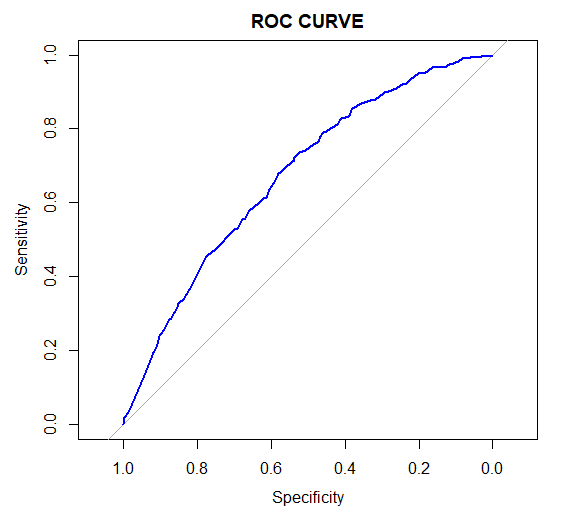
\includegraphics[scale=0.7]{images/analysis/roc.png}
	\caption{Binary Logistic Regression - ROC Curve}
	\label{roc}
\end{figure}

\noindent
The AUC (Area Under the Curve) is "0.6846". In general, a predictive model with an AUC closer to "0.5" than to "1" is quite lackluster. Still, the AUC should be interpreted in comparison to similar studies. Unfortunately, no other literature work underwent this type of analysis.
\\ \\
While in medical diagnosis the AUC should be at least "0.95", in studies related to applied psychology and prediction of future behavior, an AUC of "0.7" is a solid result.
\\ \\
Given the previous observations, I argue that the AUC found for the predictive model was poor. The reasons are the same as the ones presented for the Accuracy of the Confusion Matrix. The model is merely exploiting the binary outcome of the experiment and the imbalance between the two reaction percentages.


\newpage

\section{Conclusions}
%% CONCLUSIONS

\subsection{Phishing Survey}

The literature survey explained how phishing can ruin the lives of people from all over the world, ever since a few decades ago, even when its core concept is so straightforward. Definition, goals, taxonomy, statistics, techniques, countermeasures and trends were discussed in detail. Phishing attempts are still increasing in popularity to this day: technological defences are up to date, and now the focus should be put on phishing awareness and cybersecurity training campaigns.

\subsection{Phishing Case Study}

The case study at the University of Padua collected plenty of valuable data to assess the risk of phishing and spearphishing. The first batch of emails had a clickrate of 32\%; an outcome within the expectations, but discouraging nonetheless. The need for additional phishing awareness initiatives is very apparent. Students were the highest offenders, almost equally susceptible to generic phishing and to spearphishing. Instead, professors and technical and administrative staff members incurred in a substantially higher clickrate when targeted by spearphishing. The statistical analysis identified Age and Scenario as the most statistically significant variables, in regards to phishing susceptibility. The predictive model was ultimately inadequate and will be revisited in the future, with the addition of Education as a new predictor.
\\ \\
The phishing awareness campaign was successful, with almost 9\% of the victims fully exploring at least one educational approach. The video was more popular than the quiz but both exceeded any expectation, considering that participation was on a voluntary basis. Data from educational content was smoothly collected from the first batch of phishing emails, and is ready to be used in the next ones.

\subsection{Future Works}

The case study at the University of Padua is not over yet. I have planned two more batches of phishing emails over the next months. Thanks to the knowledge gathered in the first batch, I will be able to act more efficiently and effectively. In the next batches, I will finally test "Scenario 1 - Emails sent to Unipd as real phishing", along with the other four scenarios. I will be able to measure the impact of the phishing awareness educational campaign. The statistical analysis will be updated with future results, and I plan to improve the predictive model by adding the predictor for education. At last, I will continue monitoring phishing-related risk to which the University of Padua is currently exposed.


%---------------------------------------

\newpage

\section*{Appendix A} \hypertarget{appendix-samples}{}

\subsection*{Samples - Subjects' Dataset} \hypertarget{appendix-samples-dataset}{}

\begingroup
\renewcommand{\arraystretch}{1.25}
\begin{table}[ht!]
\begin{center}
    \begin{tabular}{ | c | l | l | l | l | }
    \hline
    \textbf{Email} & \textbf{Age} & \textbf{Gender} & \textbf{Category} & \textbf{Subcategory (Department)} \\
    \hline
    user.1@unipd.it & 24 & F & Student & Department of Mathematics \\
    \hline
    user.2@unipd.it & 22 & F & Student & Department of Mathematics \\
    \hline
    user.3@unipd.it & 25 & M & Student & Department of Mathematics \\
    \hline
    ... & ... & ... & ... & ... \\
    \hline
    user.145@unipd.it & 21 & F & Student & Department of Physics and Astronomy \\
    \hline
    user.146@unipd.it & 23 & F & Student & Department of Physics and Astronomy \\
    \hline
    ... & ... & ... & ... & ... \\
    \hline
    user.238@unipd.it & 24 & M & Student & Department of General Psychology \\
    \hline
    ... & ... & ... & ... & ... \\
    \hline
    user.450@unipd.it & 22 & F & Student & Department of Geosciences \\
    \hline
    ... & ... & ... & ... & ... \\
    \hline
    user.601@unipd.it & 22 & M & Student & Department of Molecular Medicine \\
    \hline
    ... & ... & ... & ... & ... \\
    \hline
    user.725@unipd.it & 21 & F & Student & Department of Biology \\
    \hline
    ... & ... & ... & ... & ... \\
    \hline
    user.4400@unipd.it & 24 & M & Student & Department of Statistical Sciences \\
    \hline
    ... & ... & ... & ... & ... \\
    \hline
    user.5000@unipd.it & 25 & F & Student & Department of Industrial Engineering \\
    \hline
    \end{tabular}
\end{center}
\caption{Students Dataset Sample}
\label{t-stud-sample}
\end{table}

\newpage

\begingroup
\renewcommand{\arraystretch}{1.25}
\begin{table}[ht]
\begin{center}
    \begin{tabular}{ | c | l | l | l | l | l | }
    \hline
    \textbf{Email} & \textbf{Age} & \textbf{Gender} & \textbf{Category} & \textbf{Subcategory (Macro-area)} \\
    \hline
    user.5501@unipd.it & 41 & M & Professor & Pure Science \\
    \hline
    user.5502@unipd.it & 43 & M & Professor & Pure Science \\
    \hline
    user.5503@unipd.it & 43 & M & Professor & Pure Science \\
    \hline
    user.5504@unipd.it & 43 & M & Professor & Pure Science \\
    \hline
    ... & ... & ... & ... & ... \\
    \hline
    user.5665@unipd.it & 32 & F & Professor & Pure Science \\
    \hline
    user.5666@unipd.it & 39 & M & Professor & Life Science \\
    \hline
    user.5667@unipd.it & 55 & M & Professor & Life Science \\
    \hline
    user.5668@unipd.it & 49 & M & Professor & Life Science \\
    \hline
    user.5669@unipd.it & 49 & M & Professor & Life Science \\
    \hline
    ... & ... & ... & ... & ... \\
    \hline
    user.5665@unipd.it & 32 & F & Professor & Life Science \\
    \hline
    user.5666@unipd.it & 39 & M & Professor & Human and Social Science \\
    \hline
    user.5667@unipd.it & 55 & M & Professor & Human and Social Science \\
    \hline
    user.5668@unipd.it & 49 & M & Professor & Human and Social Science \\
    \hline
    user.5669@unipd.it & 49 & M & Professor & Human and Social Science \\
    \hline
    ... & ... & ... & ... & ... \\
    \hline
    user.6000@unipd.it & 37 & F & Professor & Human and Social Science \\
    \hline
    \end{tabular}
\end{center}
\caption{Professors Dataset Sample}
\label{t-doc-sample}
\end{table}

\bigskip

\begingroup
\renewcommand{\arraystretch}{1.25}
\begin{table}[ht!]
\begin{center}
    \begin{tabular}{ | c | l | l | l | l | l | }
    \hline
    \textbf{Email} & \textbf{Age} & \textbf{Gender} & \textbf{Category} & \textbf{Subcategory (Job Description)} \\
    \hline
    user.5001@unipd.it & 25 & M & TA Staff & Administrative \\
    \hline
    user.5002@unipd.it & 43 & F & TA Staff & Administrative \\
    \hline
    user.5003@unipd.it & 29 & F & TA Staff & Administrative \\
    \hline
    user.5004@unipd.it & 50 & F & TA Staff & Administrative \\
    \hline
    user.5004@unipd.it & 51 & M & TA Staff & Administrative \\
    \hline
    user.5004@unipd.it & 32 & F & TA Staff & Administrative \\
    \hline
    ... & ... & ... & ... & ... \\
    \hline
    user.5321@unipd.it & 56 & F & TA Staff & Administrative \\
    \hline
    user.5322@unipd.it & 33 & M & TA Staff & Technical \\
    \hline
    user.5323@unipd.it & 61 & M & TA Staff & Technical \\
    \hline
    user.5324@unipd.it & 45 & F & TA Staff & Technical \\
    \hline
    user.5325@unipd.it & 48 & M & TA Staff & Technical \\
    \hline
    user.5326@unipd.it & 38 & M & TA Staff & Technical \\
    \hline
    ... & ... & ... & ... & ... \\
    \hline
    user.5500@unipd.it & 30 & M & TA Staff & Technical \\
    \hline
    \end{tabular}
\end{center}
\caption{Technical and Administrative Dataset Sample}
\label{t-ta-sample}
\end{table}

\newpage

\subsection*{Samples - Results} \hypertarget{appendix-samples-results}{}

\begingroup
\renewcommand{\arraystretch}{1.25}
\begin{table}[ht]
\begin{center}
    \begin{tabular}{ | c | l | l | l | l | l | }
    \hline
    \textbf{Email} & \textbf{Reaction} & \textbf{Timestamp} & \textbf{Batch} & \textbf{Template} & \textbf{Edu} \\
    \hline
    user.5504@unipd.it & - & - & 1st & reale-supporto & - \\
    \hline
    user.5504@unipd.it & - & - & 2nd & reale-uscite & - \\
    \hline
    user.5504@unipd.it & - & - & 3rd & reale-manutenzione & - \\
    \hline
    user.5369@unipd.it & Clicked & 03-12T09:23 & 1st & standard-sicurezza & None \\
    \hline
    user.5357@unipd.it & - & - & 2nd & standard-dropbox & Quiz \\
    \hline
    user.5357@unipd.it & - & - & 3rd & standard-accesso & Quiz \\
    \hline
    user.4800@unipd.it & - & 03-12T13:13 & 1st & mir-stud-appello & None \\
    \hline
    user.4800@unipd.it & - & - & 2nd & mir-stud-password & None \\
    \hline
    user.4800@unipd.it & - & - & 3rd & mir-stud-linkedin & - \\
    \hline
    user.33@unipd.it & Clicked & 03-13T09:23 & 1st & mir-stud-appello & None \\
    \hline
    user.33@unipd.it & - & - & 2nd & mir-stud-password & Quiz \\
    \hline
    user.33@unipd.it & - & - & 3rd & mir-stud-linkedin & Quiz \\
    \hline
    user.5604@unipd.it & Clicked & 03-13T17:37 & 1st & mir-doc-paper & None \\
    \hline
    user.5604@unipd.it & - & - & 2nd & mir-doc-convenzioni & Video \\
    \hline
    user.5604@unipd.it & - & - & 3rd & mir-doc-researchgate & Video \\
    \hline
    user.5186@unipd.it & Clicked & 03-13T21:45 & 1st & mir-pta-drive & None \\
    \hline
    user.5186@unipd.it & - & - & 2nd & mir-pta-office & Both \\
    \hline
    user.5186@unipd.it & - & - & 3rd & mir-pta-satisfaction & Both \\
    \hline
    \end{tabular}
\end{center}
\caption{Phishing Assessment Results Sample - After First Batch}
\label{t-res-sample}
\end{table}

\newpage

\section*{Appendix B} \hypertarget{appendix-varreact}{}

\subsection*{Raw Results - After First Batch}

\subsubsection*{Reaction - Overview}

\begingroup
\renewcommand{\arraystretch}{1.25}
\begin{table}[ht]
\begin{center}
    \begin{tabular}{ | m{12.3em} | m{12.3em} | m{12.3em} | }
    \hline
    \multicolumn{3}{|l|}{\textbf{Grand Total}} \\
    \hline
    Delivered & Clicked & Not Clicked \\
    \hline
    \textit{1016} & \textit{319 (31\%)} & \textit{697 (69\%)} \\
    \hline
    \end{tabular}
\end{center}
\caption{Phishing Assessment Raw Results - Reaction - Grand Total}
\label{t-varreact0-grandtotal}
\end{table}

\vspace{10mm}

\begingroup
\renewcommand{\arraystretch}{1.25}
\begin{table}[ht]
\begin{center}
    \begin{tabular}{ | m{12.3em} | m{12.3em} | m{12.3em} | }
    \hline
    \multicolumn{3}{|l|}{\textbf{Scenario 1 - Emails sent to Unipd as real phishing}} \\
    \hline
    Delivered & Clicked & Not Clicked \\
    \hline
    \textit{0} & \textit{-} & \textit{-} \\
    \hline
    \multicolumn{3}{|l|}{\textbf{Scenario 2 - Emails not tailored for any specific demographic}} \\
    \hline
    Delivered & Clicked & Not Clicked \\
    \hline
    \textit{488} & \textit{127 (26\%)} & \textit{361 (74\%)} \\
    \hline
    \multicolumn{3}{|l|}{\textbf{Scenario 3 - Emails specifically tailored to students}} \\
    \hline
    Delivered & Clicked & Not Clicked \\
    \hline
    \textit{200} & \textit{85 (43\%)} & \textit{115 (57\%)} \\
    \hline
    \multicolumn{3}{|l|}{\textbf{Scenario 4 - Emails specifically tailored to professors}} \\
    \hline
    Delivered & Clicked & Not Clicked \\
    \hline
    \textit{164} & \textit{53 (32\%)} & \textit{111 (68\%)} \\
    \hline
    \multicolumn{3}{|l|}{\textbf{Scenario 5 - Emails specifically tailored to technical and administrative staff}} \\
    \hline
    Delivered & Clicked & Not Clicked \\
    \hline
    \textit{164} & \textit{54 (33\%)} & \textit{110 (67\%)} \\
    \hline
    \end{tabular}
\end{center}
\caption{Phishing Assessment Raw Results - Reaction - Scenarios}
\label{t-varreact0-scen}
\end{table}

\vspace{5mm}

\begin{figure}[H]
	\centering
	\fbox{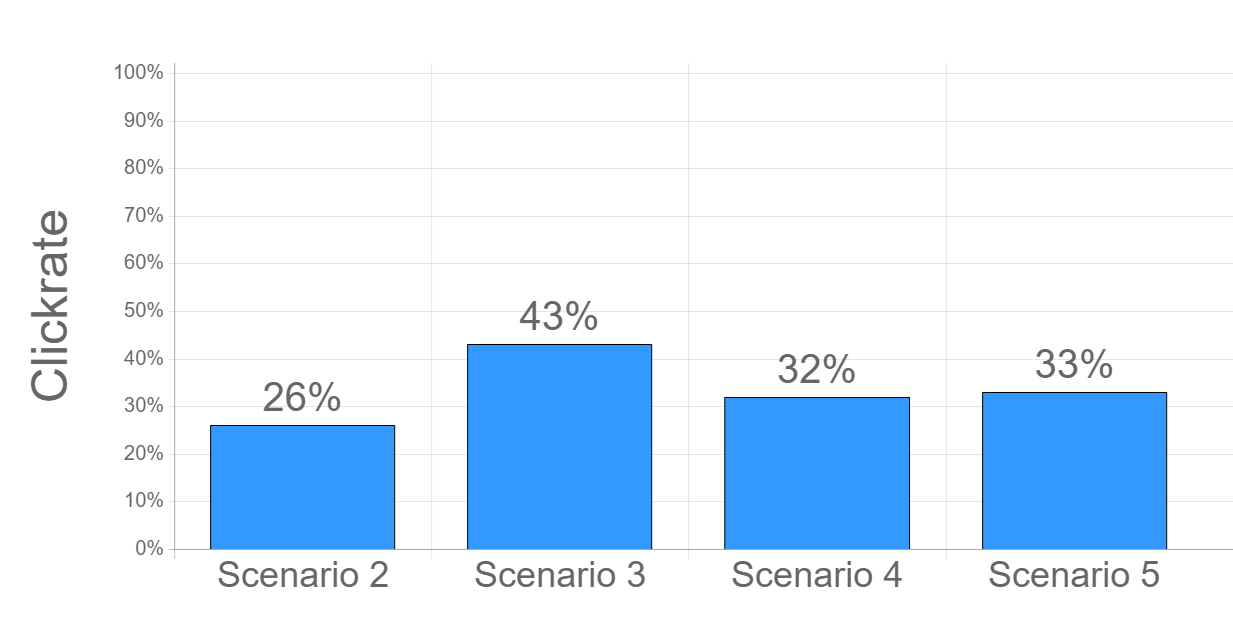
\includegraphics[scale=0.28]{images/charts/chart-scen.PNG}}
	\caption{Phishing Assessment Raw Results - Scenario/Clickrate Chart}
	\label{chart-scen}
\end{figure}

\newpage

\begingroup
\renewcommand{\arraystretch}{1.25}
\begin{table}[ht]
\begin{center}
    \begin{tabular}{ | m{12.3em} | m{12.3em} | m{12.3em} | }
    \hline
    \multicolumn{3}{|l|}{\textbf{Students Only}} \\
    \hline
    Delivered & Clicked & Not Clicked \\
    \hline
    \textit{360} & \textit{160 (44\%)} & \textit{200 (56\%)} \\
    \hline
    \multicolumn{3}{|l|}{\textbf{Professors Only}} \\
    \hline
    Delivered & Clicked & Not Clicked \\
    \hline
    \textit{328} & \textit{75 (23\%)} & \textit{253 (77\%)} \\
    \hline
    \multicolumn{3}{|l|}{\textbf{Technical and Administrative Staff Only}} \\
    \hline
    Delivered & Clicked & Not Clicked \\
    \hline
    \textit{328} & \textit{84 (26\%)} & \textit{244 (74\%)} \\
    \hline
    \end{tabular}
\end{center}
\caption{Phishing Assessment Raw Results - Reaction - Categories}
\label{t-varreact0-cat}
\end{table}

\vspace{5mm}

\begin{figure}[H]
	\centering
	\fbox{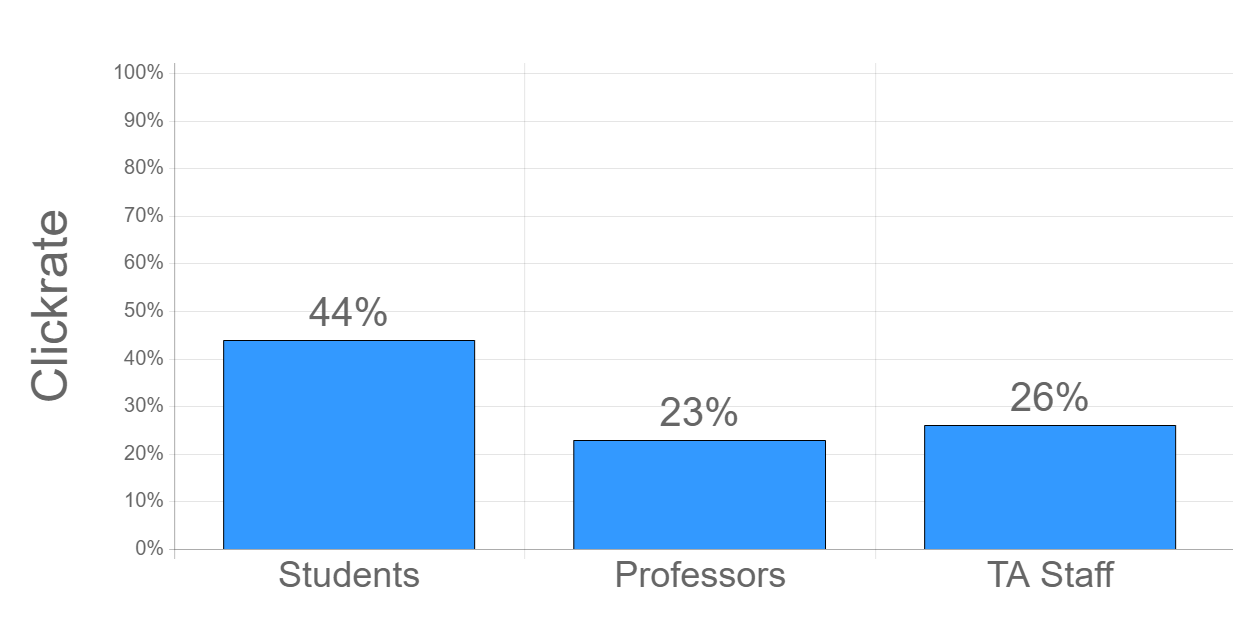
\includegraphics[width=\linewidth]{images/charts/chart-cat.PNG}}
	\caption{Phishing Assessment Raw Results - Category/Clickrate Chart}
	\label{chart-cat}
\end{figure}

\newpage

\subsubsection*{Variable/Reaction - All Scenarios}

\begingroup
\renewcommand{\arraystretch}{1.25}
\begin{table}[ht]
\begin{center}
    \begin{tabular}{ | m{7em} | m{9em} | m{9em} | m{9em} | }
    \hline
    \multicolumn{4}{|c|}{\textbf{All Scenarios (S2-S3-S4-S5)}} \\ \hline
    & & \multicolumn{2}{|c|}{\textbf{All Templates}} \\ \hline
    & & Clicked & Not Clicked \\ \hline
    
    \multirow{2}{*}{\textbf{Gender}} 
    & Male & \textit{151 (30\%)} & \textit{360 (70\%)} \\ \cline{2-4}
    & Female & \textit{168 (33\%)} & \textit{337 (67\%)} \\ \hline
    
    \multirow{5}{*}{\textbf{Age}} 
    & 0-20 & \textit{26 (55\%)} & \textit{21 (45\%)} \\ \cline{2-4}
    & 21-25 & \textit{105 (48\%)} & \textit{116 (52\%)} \\ \cline{2-4}
    & 26-30 & \textit{26 (37\%)} & \textit{44 (63\%)} \\ \cline{2-4}
    & 31-35 & \textit{17 (27\%)} & \textit{46 (73\%)} \\ \cline{2-4}
    & 36-40 & \textit{17 (20\%)} & \textit{70 (80\%)} \\ \cline{2-4}
    & 41-45 & \textit{27 (25\%)} & \textit{80 (75\%)} \\ \cline{2-4}
    & 46-50 & \textit{36 (29\%)} & \textit{89 (71\%)} \\ \cline{2-4}
    & 51-55 & \textit{35 (27\%)} & \textit{97 (73\%)} \\ \cline{2-4}
    & 56-60 & \textit{19 (23\%)} & \textit{62 (77\%)} \\ \cline{2-4}
    & 61-99 & \textit{11 (13\%)} & \textit{72 (87\%)} \\ \hline
    
    \multirow{3}{*}{\textbf{Category}} 
    & Student & \textit{160 (44\%)} & \textit{200 (56\%)} \\ \cline{2-4}
    & Professor & \textit{75 (23\%)} & \textit{253 (77\%)} \\ \cline{2-4}
    & TA Staff & \textit{84 (26\%)} & \textit{244 (74\%)} \\ \hline
    
    \multirow{1}{*}{\textbf{Education}}
    & None & \textit{-} & \textit{-} \\ \hline
    \end{tabular}
\end{center}
\caption{Phishing Assessment Raw Results - Variable/Reaction - All Scenarios}
\label{t-varreact1}
\end{table}
\endgroup

\vspace{5mm}

\begin{figure}[H]
	\centering
	\fbox{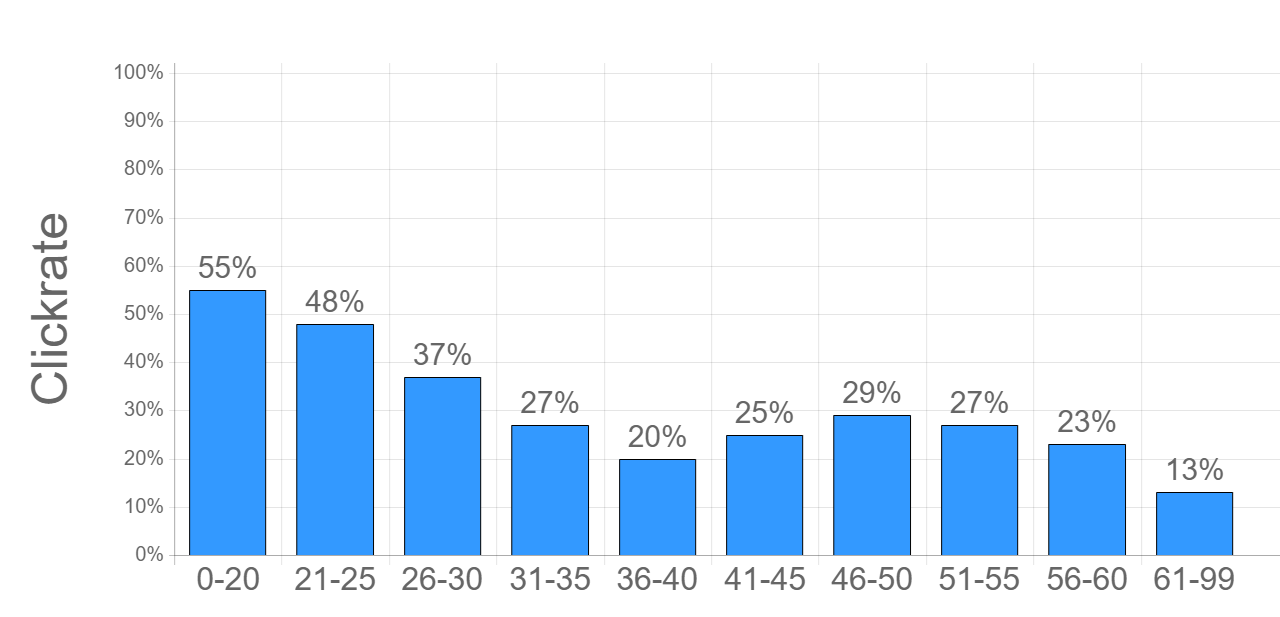
\includegraphics[width=\linewidth]{images/charts/chart-age-alls.PNG}}
	\caption{Phishing Assessment Raw Results - Age/Reaction Chart - All Scenarios}
	\label{chart-age-alls}
\end{figure}

\newpage

\subsubsection*{Variable/Reaction - Scenario 2}

\begingroup
\renewcommand{\arraystretch}{1.25}
\begin{table}[ht]
\begin{center}
    \begin{tabular}{ | m{7em} | m{9em} | m{9em} | m{9em} | }
    \hline
    \multicolumn{4}{|c|}{\textbf{Scenario 2 - Emails not tailored for any specific demographic}} \\ \hline
    & & \multicolumn{2}{|c|}{\textbf{Template "standard-sicurezza"}} \\ \hline
    & & Clicked & Not Clicked \\ \hline
    
    \multirow{2}{*}{\textbf{Gender}} 
    & Male & \textit{61 (25\%)} & \textit{184 (75\%)} \\ \cline{2-4}
    & Female & \textit{66 (27\%)} & \textit{177 (73\%)} \\ \hline
    
    \multirow{5}{*}{\textbf{Age}} 
    & 0-20 & \textit{10 (53\%)} & \textit{9 (47\%)} \\ \cline{2-4}
    & 21-25 & \textit{48 (49\%)} & \textit{50 (51\%)} \\ \cline{2-4}
    & 26-30 & \textit{14 (41\%)} & \textit{20 (59\%)} \\ \cline{2-4}
    & 31-35 & \textit{9 (26\%)} & \textit{25 (74\%)} \\ \cline{2-4}
    & 36-40 & \textit{4 (10\%)} & \textit{35 (90\%)} \\ \cline{2-4}
    & 41-45 & \textit{4 (9\%)} & \textit{41 (91\%)} \\ \cline{2-4}
    & 46-50 & \textit{16 (22\%)} & \textit{56 (78\%)} \\ \cline{2-4}
    & 51-55 & \textit{12 (19\%)} & \textit{51 (81\%)} \\ \cline{2-4}
    & 56-60 & \textit{8 (20\%)} & \textit{31 (80\%)} \\ \cline{2-4}
    & 61-99 & \textit{2 (5\%)} & \textit{41 (95\%)} \\ \hline
    
    \multirow{3}{*}{\textbf{Category}} 
    & Student & \textit{75 (47\%)} & \textit{85 (53\%)} \\ \cline{2-4}
    & Professor & \textit{22 (13\%)} & \textit{142 (87\%)} \\ \cline{2-4}
    & TA Staff & \textit{30 (18\%)} & \textit{134 (82\%)} \\ \hline
    
    \multirow{1}{*}{\textbf{Education}}
    & None & \textit{-} & \textit{-} \\ \hline
    \end{tabular}
\end{center}
\caption{Phishing Assessment Raw Results - Variable/Reaction - Scenario 2}
\label{t-varreact2}
\end{table}
\endgroup

\vspace{5mm}

\begin{figure}[H]
	\centering
	\fbox{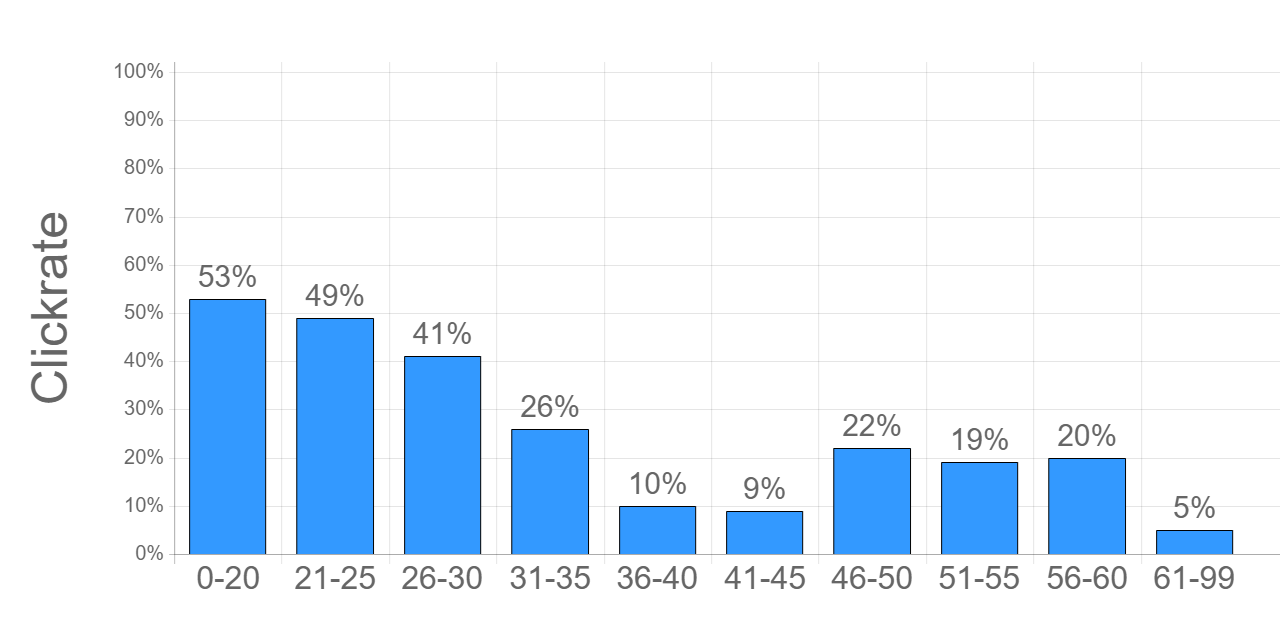
\includegraphics[width=\linewidth]{images/charts/chart-age-s2.PNG}}
	\caption{Phishing Assessment Raw Results - Age/Reaction Chart - Scenario 2}
	\label{chart-age-s2}
\end{figure}

\newpage

\subsubsection*{Variable/Reaction - Scenario 3}

\begingroup
\renewcommand{\arraystretch}{1.25}
\begin{table}[ht]
\begin{center}
    \begin{tabular}{ | m{7em} | m{9em} | m{9em} | m{9em} | }
    \hline
    \multicolumn{4}{|c|}{\textbf{Scenario 3 - Emails specifically tailored to students}} \\ \hline
    & & \multicolumn{2}{|c|}{\textbf{Template "mir-stud-appello"}} \\ \hline
    & & Clicked & Not Clicked \\ \hline
    
    \multirow{2}{*}{\textbf{Gender}} 
    & Male & \textit{36 (37\%)} & \textit{61 (63\%)} \\ \cline{2-4}
    & Female & \textit{49 (48\%)} & \textit{54 (52\%)} \\ \hline
    
    \multirow{5}{*}{\textbf{Age}} 
    & 0-20 & \textit{16 (57\%)} & \textit{12 (43\%)} \\ \cline{2-4}
    & 21-25 & \textit{57 (46\%)} & \textit{66 (54\%)} \\ \cline{2-4}
    & 26-30 & \textit{9 (30\%)} & \textit{21 (70\%)} \\ \cline{2-4}
    & 31-35 & \textit{2 (29\%)} & \textit{5 (71\%)} \\ \cline{2-4}
    & 36-40 & \textit{0 (0\%)} & \textit{4 (100\%)} \\ \cline{2-4}
    & 41-45 & \textit{1 (25\%)} & \textit{3 (75\%)} \\ \cline{2-4}
    & 46-50 & \textit{0 (0\%)} & \textit{2 (100\%)} \\ \cline{2-4}
    & 51-55 & \textit{0 (0\%)} & \textit{1 (100\%)} \\ \cline{2-4}
    & 56-60 & \textit{-} & \textit{-} \\ \cline{2-4}
    & 61-99 & \textit{0 (0\%)} & \textit{1 (100\%)} \\ \hline
    
    \multirow{1}{*}{\textbf{Category}}
    & Student & \textit{85 (43\%)} & \textit{115 (57\%)} \\ \hline
    
    \multirow{1}{*}{\textbf{Education}}
    & None & \textit{-} & \textit{-} \\ \hline
    \end{tabular}
\end{center}
\caption{Phishing Assessment Raw Results - Variable/Reaction - Scenario 3}
\label{t-varreact3}
\end{table}
\endgroup

\vspace{5mm}

\begin{figure}[H]
	\centering
	\fbox{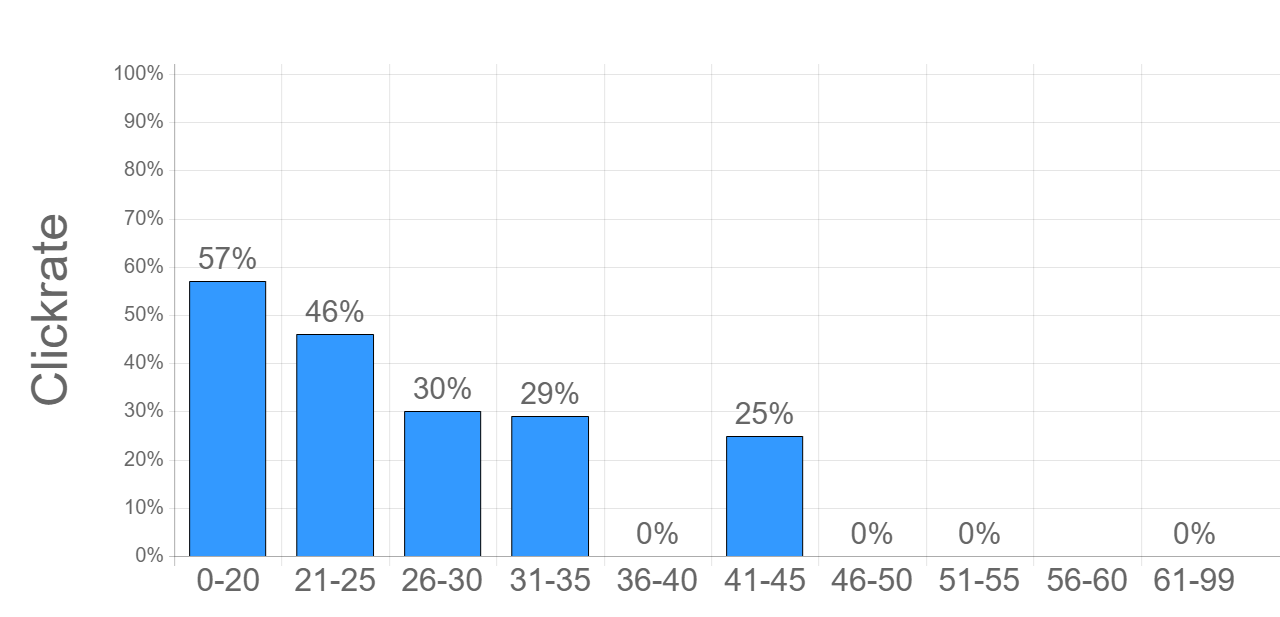
\includegraphics[width=\linewidth]{images/charts/chart-age-s3.PNG}}
	\caption{Phishing Assessment Raw Results - Age/Reaction Chart - Scenario 3}
	\label{chart-age-s3}
\end{figure}

\newpage

\subsubsection*{Variable/Reaction - Scenario 4}

\begingroup
\renewcommand{\arraystretch}{1.25}
\begin{table}[ht]
\begin{center}
    \begin{tabular}{ | m{7em} | m{9em} | m{9em} | m{9em} | }
    \hline
    \multicolumn{4}{|c|}{\textbf{Scenario 4 - Emails specifically tailored to professors}} \\ \hline
    & & \multicolumn{2}{|c|}{\textbf{Template "mir-doc-paper"}} \\ \hline
    & & Clicked & Not Clicked \\ \hline
    
    \multirow{2}{*}{\textbf{Gender}} 
    & Male & \textit{33 (32\%)} & \textit{69 (68\%)} \\ \cline{2-4}
    & Female & \textit{20 (32\%)} & \textit{42 (68\%)} \\ \hline
    
    \multirow{5}{*}{\textbf{Age}} 
    & 0-20 & \textit{-} & \textit{-} \\ \cline{2-4}
    & 21-25 & \textit{-} & \textit{-} \\ \cline{2-4}
    & 26-30 & \textit{-} & \textit{-} \\ \cline{2-4}
    & 31-35 & \textit{2 (40\%)} & \textit{3 (60\%)} \\ \cline{2-4}
    & 36-40 & \textit{5 (19\%)} & \textit{22 (81\%)} \\ \cline{2-4}
    & 41-45 & \textit{11 (37\%)} & \textit{19 (63\%)} \\ \cline{2-4}
    & 46-50 & \textit{11 (42\%)} & \textit{15 (58\%)} \\ \cline{2-4}
    & 51-55 & \textit{10 (33\%)} & \textit{20 (67\%)} \\ \cline{2-4}
    & 56-60 & \textit{5 (29\%)} & \textit{12 (71\%)} \\ \cline{2-4}
    & 61-99 & \textit{9 (31\%)} & \textit{20 (69\%)} \\ \hline
   
    \multirow{1}{*}{\textbf{Category}} 
    & Professor & \textit{53 (32\%)} & \textit{111 (68\%)} \\ \hline
    
    \multirow{1}{*}{\textbf{Education}}
    & None & \textit{-} & \textit{-} \\ \hline
    \end{tabular}
\end{center}
\caption{Phishing Assessment Raw Results - Variable/Reaction - Scenario 4}
\label{t-varreact4}
\end{table}
\endgroup

\vspace{5mm}

\begin{figure}[H]
	\centering
	\fbox{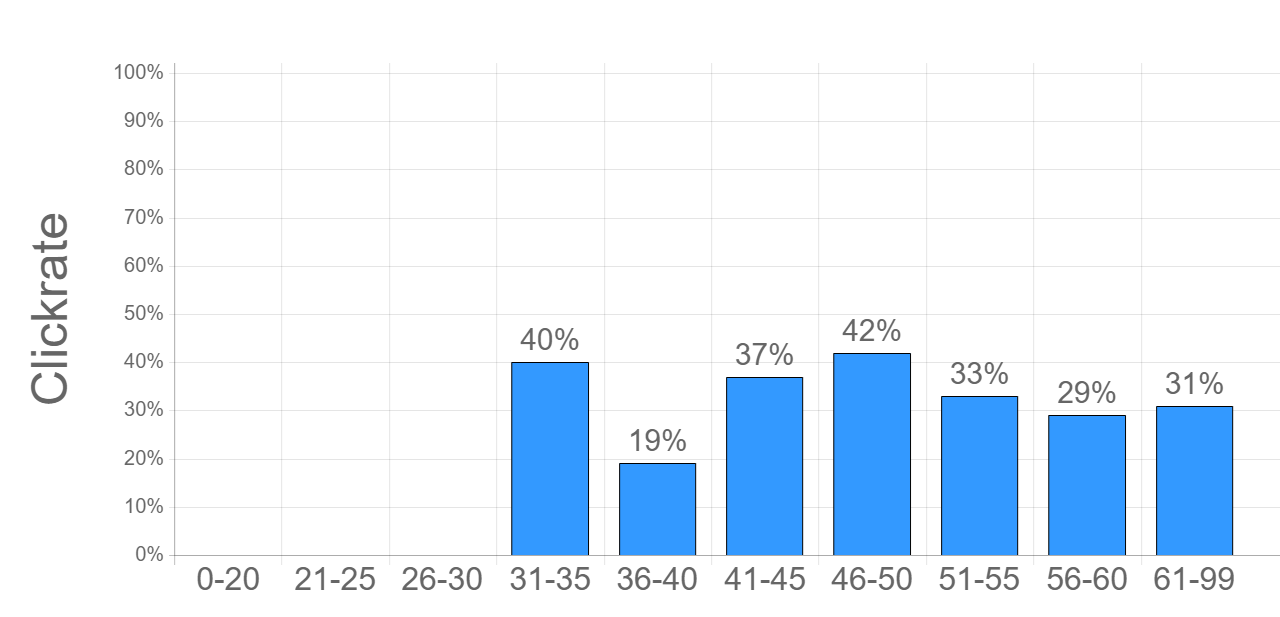
\includegraphics[width=\linewidth]{images/charts/chart-age-s4.PNG}}
	\caption{Phishing Assessment Raw Results - Age/Reaction Chart - Scenario 4}
	\label{chart-age-s4}
\end{figure}

\newpage

\subsubsection*{Variable/Reaction - Scenario 5}

\begingroup
\renewcommand{\arraystretch}{1.25}
\begin{table}[ht]
\begin{center}
    \begin{tabular}{ | m{7em} | m{9em} | m{9em} | m{9em} | }
    \hline
    \multicolumn{4}{|c|}{\textbf{Scenario 5 -  Emails specifically tailored to technical and administrative staff}} \\ \hline
    & & \multicolumn{2}{|c|}{\textbf{Template "mir-pta-drive"}} \\ \hline
    & & Clicked & Not Clicked \\ \hline
    
    \multirow{2}{*}{\textbf{Gender}} 
    & Male & \textit{21 (31\%)} & \textit{46 (69\%)} \\ \cline{2-4}
    & Female & \textit{33 (34\%)} & \textit{64 (66\%)} \\ \hline
    
    \multirow{5}{*}{\textbf{Age}} 
    & 0-20 & \textit{-} & \textit{-} \\ \cline{2-4}
    & 21-25 & \textit{-} & \textit{-} \\ \cline{2-4}
    & 26-30 & \textit{3 (50\%)} & \textit{3 (50\%)} \\ \cline{2-4}
    & 31-35 & \textit{4 (24\%)} & \textit{13 (76\%)} \\ \cline{2-4}
    & 36-40 & \textit{8 (47\%)} & \textit{9 (53\%)} \\ \cline{2-4}
    & 41-45 & \textit{11 (39\%)} & \textit{17 (61\%)} \\ \cline{2-4}
    & 46-50 & \textit{9 (36\%)} & \textit{16 (64\%)} \\ \cline{2-4}
    & 51-55 & \textit{13 (35\%)} & \textit{24 (65\%)} \\ \cline{2-4}
    & 56-60 & \textit{6 (25\%)} & \textit{18 (75\%)} \\ \cline{2-4}
    & 61-99 & \textit{0 (0\%)} & \textit{10 (100\%)} \\ \hline
    
    \multirow{1}{*}{\textbf{Category}} 
    & TA Staff & \textit{54 (33\%)} & \textit{110 (67\%)} \\ \hline
    
    \multirow{1}{*}{\textbf{Education}}
    & None & \textit{-} & \textit{-} \\ \hline
    \end{tabular}
\end{center}
\caption{Phishing Assessment Raw Results - Variable/Reaction - Scenario 5}
\label{t-varreact5}
\end{table}
\endgroup

\vspace{5mm}

\begin{figure}[H]
	\centering
	\fbox{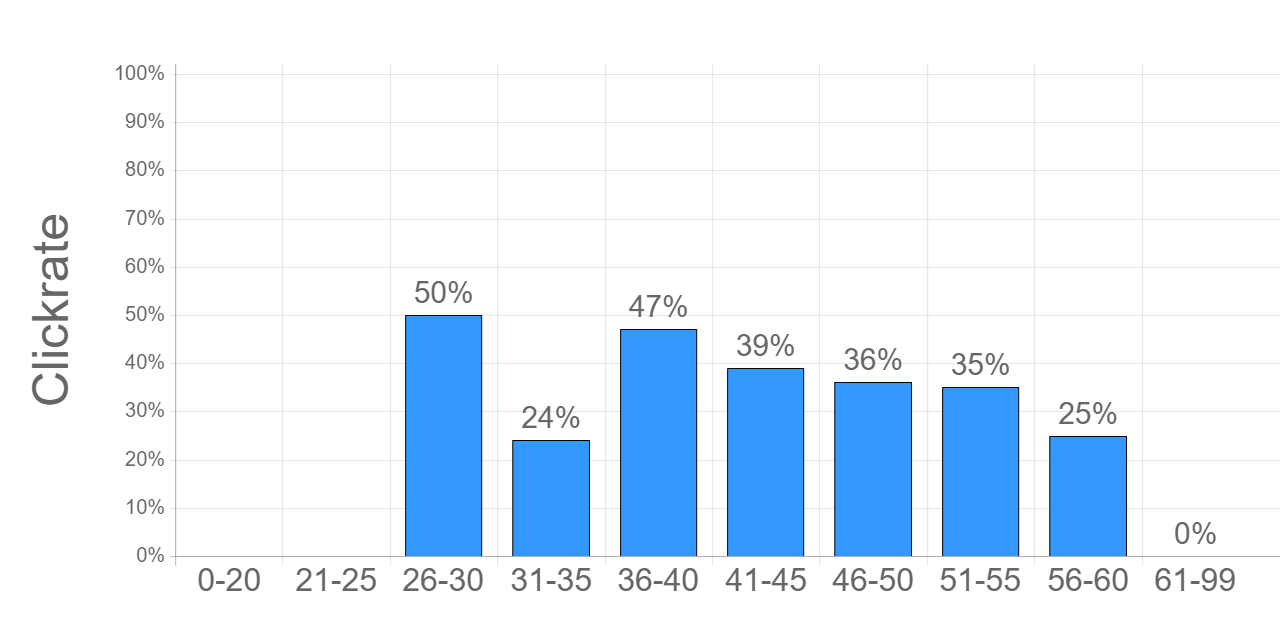
\includegraphics[width=\linewidth]{images/charts/chart-age-s5.PNG}}
	\caption{Phishing Assessment Raw Results - Age/Reaction Chart - Scenario 5}
	\label{chart-age-s5}
\end{figure}

\newpage

\subsection*{Raw Results - Education}

\begingroup
\renewcommand{\arraystretch}{1.25}
\begin{table}[ht]
\begin{center}
    \begin{tabular}{ | l | l | l | l | l | l | l | l | l | l | l | l | l | l | l | l | l | l | l | l | l | l | l | l | }
    \hline
    
    \multicolumn{24}{|l|}{\textbf{Educational Preference - Category}} \\ \hline
    \multicolumn{8}{|l|}{Student} & \multicolumn{8}{|l|}{Professor} & \multicolumn{8}{|l|}{Ta Staff} \\ \hline 
    \multicolumn{8}{|l|}{\textit{14 (56\%)}} & \multicolumn{8}{|l|}{\textit{3 (12\%)}} & \multicolumn{8}{|l|}{\textit{8 (32\%)}} \\ \hline
    \multicolumn{24}{l}{}
    \\ \hline
    
    \multicolumn{24}{|l|}{\textbf{Educational Preference - Approach}} \\ \hline
    \multicolumn{6}{|l|}{None} & \multicolumn{6}{|l|}{Video Only} & \multicolumn{6}{|l|}{Quiz Only} & \multicolumn{6}{|l|}{Video and Quiz} \\
    \hline
    \multicolumn{6}{|l|}{\textit{291 (91\%)}} & \multicolumn{6}{|l|}{\textit{17 (5\%)}} & \multicolumn{6}{|l|}{\textit{8 (3\%)}} & \multicolumn{6}{|l|}{\textit{3 (1\%)}} \\ \hline
    \multicolumn{24}{l}{}
    \\ \hline
    
    \multicolumn{24}{|l|}{\textbf{Quiz - Score Distributions}} \\ \hline
    \multicolumn{3}{|l|}{Zero} & \multicolumn{3}{|l|}{One} & \multicolumn{3}{|l|}{Two} & \multicolumn{3}{|l|}{Three} & \multicolumn{3}{|l|}{Four} & \multicolumn{3}{|l|}{Five} & \multicolumn{3}{|l|}{Six} & \multicolumn{3}{|l|}{Seven} \\
    \hline
    \multicolumn{3}{|l|}{\textit{0 (0\%)}} & \multicolumn{3}{|l|}{\textit{0 (0\%)}} & \multicolumn{3}{|l|}{\textit{0 (0\%)}} & \multicolumn{3}{|l|}{\textit{0 (0\%)}} & \multicolumn{3}{|l|}{\textit{2 (18\%)}} & \multicolumn{3}{|l|}{\textit{7 (64\%)}} & \multicolumn{3}{|l|}{\textit{2 (18\%)}} & \multicolumn{3}{|l|}{\textit{0 (0\%)}} \\
    \hline
    
    \end{tabular}
\end{center}
\caption{Phishing Assessment Raw Results - Education - After First Batch}
\label{t-varreact-edu}
\end{table}

\newpage

\section*{Appendix C}

\subsection*{Data Analysis - R Code}

The following code was used to retrieve the statistical data, to execute Chi-Squared tests and to model the Binary Logistic Regression presented in "Results, Analysis and Interpretation". The following code was written in R, and was ran inside RStudio \cite{tools-rstudio}:

\begin{lstlisting}
   
library(dplyr) #between
library(plyr) #revalue
library(expss) #count_if
library(MASS) #glm
library(pROC) # roc curve

#dataset
personal_stud <- read.csv(file.path("Dati Soggetti Gophish/Dataset/","studenti.csv"),sep=';')
personal_prof <- read.csv(file.path("Dati Soggetti Gophish/Dataset/","docenti.csv"),sep=';')
personal_ta <- read.csv(file.path("Dati Soggetti Gophish/Dataset/","pta.csv"),sep=';')

##gophish results s1
##stud_s1_results <- read.csv(file.path("Dati Soggetti Gophish/Risultati/Studenti/","S1 - Reale - Supporto Limite Quote - Studenti - Results.csv"),sep=',')
##prof_s1_results <- read.csv(file.path("Dati Soggetti Gophish/Risultati/Docenti/","S1 - Reale - Supporto Limite Quote - Docenti - Results.csv"),sep=',')
##ta_s1_results <- read.csv(file.path("Dati Soggetti Gophish/Risultati/PTA/","S1 - Reale - Supporto Limite Quote - PTA - Results.csv"),sep=',')


#gophish results s2
results_s2_stud <- read.csv(file.path("Dati Soggetti Gophish/Risultati/Studenti/","S2 - Standard - Google Avviso Sicurezza - Studenti - Results.csv"),sep=',')
results_s2_prof <- read.csv(file.path("Dati Soggetti Gophish/Risultati/Docenti/","S2 - Standard - Google Avviso Sicurezza - Docenti - Results.csv"),sep=',')
results_s2_ta <- read.csv(file.path("Dati Soggetti Gophish/Risultati/PTA/","S2 - Standard - Google Avviso Sicurezza - PTA - Results.csv"),sep=',')

#gophish results s3-s4-s5
results_s3_stud <- read.csv(file.path("Dati Soggetti Gophish/Risultati/Studenti/","S3 - Mirato Studenti - Risultato Esame - Studenti - Results.csv"),sep=',')
results_s4_prof <- read.csv(file.path("Dati Soggetti Gophish/Risultati/Docenti/","S4 - Mirato Docenti - Richiesta Paper - Docenti - Results.csv"),sep=',')
results_s5_ta <- read.csv(file.path("Dati Soggetti Gophish/Risultati/PTA/","S5 - Mirato PTA - Condivisione Drive - PTA - Results.csv"),sep=',')

#function merging a list
list_merging <- function(merge_list) {
  
  #merge stats_list in one dataframe
  return (Reduce(function(x,y) merge(x,y,all=TRUE),merge_list))
  
}

#function renaming results colnames
colrename <- function(results) {
  
  #rename columns
  names(results)[colnames(results) == 'email'] <- 'Email'
  names(results)[colnames(results) == 'id'] <- 'Rid'
  names(results)[colnames(results) == 'status'] <- 'Reaction'
  
  return (results)
  
}

#function creating aggregated data, personal+results
aggregation <- function(personal,results) {
  
  #outer join on Email, adds personal information
  complete<-merge(x=personal,y=results,by="Email",all=TRUE)
  
  #delete unused columns
  complete[8:16] <- list(NULL)
  
  #renaming fields
  complete$Reaction <- revalue(complete$Reaction,c("Email Opened"="Delivered"))
  complete$Reaction <- revalue(complete$Reaction,c("Email Sent"="Delivered"))
  complete$Reaction <- revalue(complete$Reaction,c("Clicked Link"="Clicked"))
  
  #remove undelivered
  return (complete[!is.na(complete$Reaction),])
  
}

##data aggregation s1
##personal_stud$Year <- NULL
##stud_s1_results <- colrename(stud_s1_results)
##aggreg_s1_stud <- aggregation(personal_stud,stud_s1_results)

##prof_s1_results <- colrename(prof_s1_results)
##aggreg_s1_prof <- aggregation(personal_prof,prof_s1_results)
##ta_s1_results <- colrename(ta_s1_results)
##aggreg_s1_ta <- aggregation(personal_ta,ta_s1_results)

#data aggregation s2
personal_stud$Year <- NULL
results_s2_stud <- colrename(results_s2_stud)
aggreg_s2_stud <- aggregation(personal_stud,results_s2_stud)
aggreg_s2_stud["Scenario"] <- "S2"

results_s2_prof <- colrename(results_s2_prof)
aggreg_s2_prof <- aggregation(personal_prof,results_s2_prof)
aggreg_s2_prof["Scenario"] <- "S2"

results_s2_ta <- colrename(results_s2_ta)
aggreg_s2_ta <- aggregation(personal_ta,results_s2_ta)
aggreg_s2_ta["Scenario"] <- "S2"

#data aggregation s3-s4-s5
results_s3_stud <- colrename(results_s3_stud)
aggreg_s3_stud <- aggregation(personal_stud,results_s3_stud)
aggreg_s3_stud["Scenario"] <- "S3"

results_s4_prof <- colrename(results_s4_prof)
aggreg_s4_prof <- aggregation(personal_prof,results_s4_prof)
aggreg_s4_prof["Scenario"] <- "S4"

results_s5_ta <- colrename(results_s5_ta)
aggreg_s5_ta <- aggregation(personal_ta,results_s5_ta)
aggreg_s5_ta["Scenario"] <- "S5"

#data aggregation, join by category
categ_stud_only <- list_merging(list(aggreg_s2_stud,aggreg_s3_stud)) #aggreg_s1_stud,aggreg_s2_stud,aggreg_s3_stud
categ_prof_only <- list_merging(list(aggreg_s2_prof,aggreg_s4_prof)) #aggreg_s1_prof,aggreg_s2_prof,aggreg_s4_prof
categ_ta_only <- list_merging(list(aggreg_s2_ta,aggreg_s5_ta)) #aggreg_s1_ta,aggreg_s2_ta,aggreg_s5_ta

#data aggregation, join by scenario
##scen_s1_only <- list_merging(list(aggreg_s1_stud,aggreg_s1_prof,aggreg_s1_ta))
scen_s2_only <- list_merging(list(aggreg_s2_stud,aggreg_s2_prof,aggreg_s2_ta))
scen_s3_only <- list_merging(list(aggreg_s3_stud))
scen_s4_only <- list_merging(list(aggreg_s4_prof))
scen_s5_only <- list_merging(list(aggreg_s5_ta))

#data aggregation, join everything
every_scen_and_categ <- list_merging(list(scen_s2_only,scen_s3_only,scen_s4_only,scen_s5_only)) #list(scen_s1_only,scen_s2_only,scen_s3_only,scen_s4_only,scen_s5_only)

#function calculating delivered,clicked,notclicked
metrics_calc <- function(df) {
  
  #count delivered, clicked, total
  clicked <- count_if("Clicked",df$Reaction)
  notclicked <- count_if("Delivered",df$Reaction)
  delivered <- (clicked+notclicked)
  
  #percentage clicked-notclicked
  perc_clicked <- (round((clicked/delivered)*100,digits=0))
  perc_notclicked <- (round((notclicked/delivered)*100,digits=0))
  
  #return pretty stats dataframe
  return (data.frame(delivered,clicked,perc_clicked,notclicked,perc_notclicked))
  
}

#create stats metrics scenarios
##metrics_s1 <- metrics_calc(scen_s1_only)
metrics_s2 <- metrics_calc(scen_s2_only)
metrics_s3 <- metrics_calc(scen_s3_only)
metrics_s4 <- metrics_calc(scen_s4_only)
metrics_s5 <- metrics_calc(scen_s5_only)

#create stats metrics categories
metrics_stud_only <- metrics_calc(categ_stud_only)
metrics_prof_only <- metrics_calc(categ_prof_only)
metrics_ta_only <- metrics_calc(categ_ta_only)

#create stats metrics grandtotal
metrics_grandtotal <- metrics_calc(every_scen_and_categ)

#function calculating statistics traits template
stats_varreact <- function(df) {
  
  #gender
  df_gender_male <- df[df$Gender == "M",]
  df_gender_female <- df[df$Gender == "F",]
  
  #age
  df_age_0_20 <- df[between(df$Age,0,20),]
  df_age_21_25 <- df[between(df$Age,21,25),]
  df_age_26_30 <- df[between(df$Age,26,30),]
  df_age_31_35 <- df[between(df$Age,31,35),]
  df_age_36_40 <- df[between(df$Age,36,40),]
  df_age_41_45 <- df[between(df$Age,41,45),]
  df_age_46_50 <- df[between(df$Age,46,50),]
  df_age_51_55 <- df[between(df$Age,51,55),]
  df_age_56_60 <- df[between(df$Age,56,60),]
  df_age_61_99 <- df[between(df$Age,61,99),]
  
  #category
  df_categ_stud <- df[df$Category == "studente",]
  df_categ_prof <- df[df$Category == "doc",]
  df_categ_ta <- df[df$Category == "pta",]
  
  #metrics calc gender
  male_metrics <- metrics_calc(df_gender_male)
  female_metrics <- metrics_calc(df_gender_female)
  
  #metrics calc age
  age_0_20_metrics <- metrics_calc(df_age_0_20)
  age_21_25_metrics <- metrics_calc(df_age_21_25)
  age_26_30_metrics <- metrics_calc(df_age_26_30)
  age_31_35_metrics <- metrics_calc(df_age_31_35)
  age_36_40_metrics <- metrics_calc(df_age_36_40)
  age_41_45_metrics <- metrics_calc(df_age_41_45)
  age_46_50_metrics <- metrics_calc(df_age_46_50)
  age_51_55_metrics <- metrics_calc(df_age_51_55)
  age_56_60_metrics <- metrics_calc(df_age_56_60)
  age_61_99_metrics <- metrics_calc(df_age_61_99)
  
  #metrics calc category
  categ_stud_metrics <- metrics_calc(df_categ_stud)
  categ_prof_metrics <- metrics_calc(df_categ_prof)
  categ_ta_metrics <- metrics_calc(df_categ_ta)
  
  #create return list, include every trait list
  temp_list <- list(male_metrics,female_metrics,age_0_20_metrics,age_21_25_metrics,age_26_30_metrics,age_31_35_metrics,age_36_40_metrics,age_41_45_metrics,age_46_50_metrics,age_51_55_metrics,age_56_60_metrics,age_61_99_metrics,categ_stud_metrics,categ_prof_metrics,categ_ta_metrics)
  
  #rename lists inside return list
  names(temp_list) <- c("male_metrics", "female_metrics", "age_0_20_metrics","age_21_25_metrics","age_26_30_metrics","age_31_35_metrics","age_36_40_metrics","age_41_45_metrics","age_46_50_metrics","age_51_55_metrics","age_56_60_metrics","age_61_99_metrics","categ_stud_metrics","categ_prof_metrics","categ_ta_metrics")
  
  #merge all metrics calc
  return (temp_list)
  
}

#create stats traits templates
##varreact_s1_only <- stats_varreact(scen_s1_only)
varreact_s2_only <- stats_varreact(scen_s2_only)
varreact_s3_only <- stats_varreact(scen_s3_only)
varreact_s4_only <- stats_varreact(scen_s4_only)
varreact_s5_only <- stats_varreact(scen_s5_only)

varreact_every_scen_and_categ <- stats_varreact(every_scen_and_categ)

#chi-squared
#If the p-value is less than or equal to the significance level (standard is 0.05), you reject the null hypothesis and conclude that there is a statistically significant association between the variables.
#if the p-value is larger than the significance level (standard is 0.05), you fail to reject the null hypothesis because there is not enough evidence to conclude that the variables are associated.

chi_squared_acceptance = 0.05

#function chi-squared
chi_squared <- function(df,trait) {
  
  #create table
  temp_table <- table(df$Reaction,trait)
  print(temp_table)
  
  #execute chi-squared, gender
  return (chisq.test(temp_table))
  
}

#function trait statistical significant
chi_squared_significant <- function(pvalue,trait) {
  
  #condition to be significant
  if (pvalue <= chi_squared_acceptance) {
    sprintf("Chi-squared p.value = %e >>> %s statistically significant to Reaction",pvalue,trait)
  } else {
    sprintf("Chi-squared p.value = %e >>> Not enough evidence for %s to be statistically significant to Reaction",pvalue,trait)
    
  }
}

#chi-squared gender
chisquared_gender_all <- chi_squared(every_scen_and_categ,every_scen_and_categ$Gender)
chi_squared_significant(chisquared_gender_all$p.value,"Gender")

#function age range
grouping_age <- function(age_col) {
  
  #revalue all age ranges, big ranges because low data
  age_col[between(age_col,0,20)] <- "0-20"
  age_col[between(age_col,21,25)] <- "21-25"
  age_col[between(age_col,26,30)] <- "26-30"
  age_col[between(age_col,31,35)] <- "31-35"
  age_col[between(age_col,36,40)] <- "36-40"
  age_col[between(age_col,41,45)] <- "41-45"
  age_col[between(age_col,46,50)] <- "46-50"
  age_col[between(age_col,51,55)] <- "51-55"
  age_col[between(age_col,56,60)] <- "56-60"
  age_col[between(age_col,61,99)] <- "61-99"
  
  return(age_col)
  
}

#chi-squared age
chisquared_age_all <- chi_squared(every_scen_and_categ,grouping_age(every_scen_and_categ$Age))
chi_squared_significant(chisquared_age_all$p.value,"Age")

#chi-squared category
chisquared_category_all <- chi_squared(every_scen_and_categ,every_scen_and_categ$Category)
chi_squared_significant(chisquared_category_all$p.value,"Category")

#chi-squared subcategory
chisquared_subcategory_prof <- chi_squared(categ_prof_only,categ_prof_only$Subcategory)
chi_squared_significant(chisquared_subcategory_prof$p.value,"Subcategory")

chisquared_subcategory_ta <- chi_squared(categ_ta_only,categ_ta_only$Subcategory)
chi_squared_significant(chisquared_subcategory_ta$p.value,"Subcategory")

#logistic binary regression
lbr_all <- every_scen_and_categ[!names(every_scen_and_categ) %in% c("Email","Subcategory","Rid")]
lbr_all$Age <- grouping_age(lbr_all$Age)

#estimate > 0 means more likely to click, estimate < 0 means less likely
lbr_all$Reaction <- relevel(lbr_all$Reaction,"Delivered")

#logit summary
logit <- glm(Reaction~.,family=binomial,data=lbr_all)
summary(logit)

#analysis of deviance
anova(logit,test="Chisq")

#predictive analysis
summary(logit$fitted.values)
lbr_all$Predict <- ifelse(logit$fitted.values>0.5,"Delivered","Clicked")

#confusion matrix
confusion_m <- table(lbr_all$Reaction,lbr_all$Predict)
rownames(confusion_m) <- c("Delivered","Clicked")
colnames(confusion_m) <- c("Pred. Delivered","Pred. Clicked")
confusion_m

#classification accuracy
accuracy <- sum(diag(confusion_m))/sum(confusion_m)
accuracy

#roc curve
roc(Reaction~logit$fitted.values,data=lbr_all,plot=TRUE,main="ROC CURVE",col= "blue")
    
\end{lstlisting}

\newpage
\begin{thebibliography}{1}
%% BIBLIOGRAPHY

\vspace{5mm}

% definitions

\bibitem{def-soceng-cambridge}
Cambridge Dictionary, \textit{https://dictionary.cambridge.org/dictionary/english/social-engineering}

\bibitem{def-soceng-artdeception}
Kevin D. Mittnick, William L. Simon. \emph{The Art of Deception: Controlling the Human Element of Security}, Wiley, (2002).

\bibitem{def-phishing-usgov}
US Department of Homeland Security CISA Cyber+Infrastructure,
\textit{https://www.us-cert.gov/report-phishing}

% reports

\bibitem{report-symantec}
Symantec. \emph{Internet Security Threat Report}, vol. 23, (2018).

\bibitem{report-phishme}
PhishMe Inc. \emph{Enterprise Phishing Resiliency and Defense Report}, (2017).

\bibitem{report-phishlabs-2018}
PhishLabs. \emph{2018 Phishing Trends and Intelligence (PTI) Report}, (2018).

\bibitem{report-phishlabs-2019}
PhishLabs. \emph{2019 Phishing Trends and Intelligence Report (PTI)}, (2018).

\bibitem{report-apwg}
Anti-Phishing Working Group (APWG). \emph{Phishing Activity Trends Report, 3rd Quarter 2019}, (2019).

\bibitem{report-ic3}
FBI, Internet Crime Complaint Center (IC3). \emph{2017 Internet Crime Report}, (2017).

\bibitem{report-checkpoint}
Check Point, Software Technologies LTD. \emph{2018 Security Report}, (2018).

\bibitem{report-knowbe4}
KnowBe4. \emph{2018 Phishing By Industry Benchmarking Report}, (2018).

\bibitem{report-verizon}
Verizon. \emph{2018 Data Breach Investigation Report}, (2018).

\bibitem{report-f5labs}
F5 Labs. \emph{2018 Phishing and Fraud Report: Attacks Peak During the Holidays}, (2018).

\bibitem{report-iocta}
Europol, European Cybercrime Center (EC3). \emph{2018 Internet Organized Crime Threat Assessment (IOCTA)}, (2018).

% articles

\bibitem{article-url-padding}
Crane Hassold (PhishLabs). \emph{The Mobile Phishing Threat You’ll See Very Soon: URL Padding}, https://info.phishlabs.com/blog/the-mobile-phishing-threat-youll-see-very-soon-url-padding (2017).

\bibitem{article-apple-homograph}
The Register, "That apple.com link you clicked on? Yeah, it's actually Russian", by Kieren McCarthy, \textit{https://www.theregister.co.uk/2017/04/18/homograph\_attack\_again}, (2017).

\bibitem{article-icann-homograph}
Internet Corporation for Assigned Names and Numbers (ICANN),
\textit{https://www.icann.org/news/announcement-2005-02-23-en}

\bibitem{article-silent-librarian}
Proofpoint, \textit{https://www.proofpoint.com/us/threat-insight/post/threat-actor-profile-ta407-silent-librarian}

\bibitem{article-rimasauskas}
The Guardian, \textit{https://www.theguardian.com/technology/2017/apr/28/facebook-google-conned-100m-phishing-scheme}

\bibitem{article-ukraine-power}
Wired, \textit{https://www.wired.com/2016/03/inside-cunning-unprecedented-hack-ukraines-power-grid/}

\bibitem{article-sony-breach}
Tripwire, \textit{https://www.tripwire.com/state-of-security/latest-security-news/sony-hackers-used-phishing-emails-to-breach-company-networks/}

% literature - casestudy

\bibitem{lit-casestudy-students}
Jakov Andrić, Dijana Oreški, Tonimir Kišasondi. \emph{Analysis of phishing attacks against students}, 2016 39th International Convention on Information and Communication Technology, Electronics and Microelectronics (MIPRO), pp. 1423-1429, (2016).

\bibitem{lit-casestudy-assessing-soceng}
A. Karakasiliotis, S. M. Furnell, M. Papadaki. \emph{Assessing end-user awareness of social engineering
and phishing}, 7th Australian Information Warfare and Security Conference, Edith Cowan University, Perth Western Australia, 4th - 5th December 2016, (2016).

\bibitem{lit-casestudy-assessing-resilience}
João Paulo Magalhães, António Pinto. \emph{A methodology for assessing resilience against email phishing}, 2018 International Conference on Intelligent Systems (IS), Funchal - Madeira, Portugal, 2018, pp. 515-520, (2018).

\bibitem{lit-casestudy-empirical-benefits}
Ronald C. Dodge, Kathryn Coronges, Ericka Rovira. \emph{Empirical benefits of training to phishing susceptibility}, 27th IFIP TC 11 Information Security and Privacy Conference, Heraklion, Crete, Greece, vol. 376, (2012).

\bibitem{lit-casestudy-investigation-spearphish}
Jingguo Wang, Tejaswini Herath, Rui Chen, Arun Vishwanath, H. Raghav Rao. \emph{Phishing susceptibility: an investigation into the processing of a targeted spear phishing email}, IEEE Transactions on Professional Communication, vol. 55, No. 4 (December 2012), pp. 345-362, (2012).

\bibitem{lit-casestudy-organisational-learning}
Wayne D. Kearney, Hennie A. Kruger. \emph{Phishing and organisational learning}, Security and Privacy Protection in Information Processing Systems, SEC 2013, IFIP Advances in Information and Communication Technology, vol 405. Springer, Berlin, Heidelberg, (2013).

\bibitem{lit-casestudy-ticket-solid}
Iacovos Kirlappos, M. Angela Sasse. \emph{Security education against phishing: a modest proposal for a major re-think}, IEEE Security and Privacy Magazine, March 2012, (2012).

\bibitem{lit-casestudy-revisiting-susceptibility}
T. Bakhshi. \emph{Social engineering: Revisiting end-user awareness and susceptibility to classic attack vectors}, 2017 13th International Conference on Emerging Technologies (ICET), Islamabad, 2017, pp. 1-6, (2017).

\bibitem{lit-casestudy-survey-virus}
Waldo Rocha Flores, Hannes Holm, Gustav Svensson, G. N. Ericsson, G. N. Ericsson. \emph{Using phishing experiments and scenario-based surveys to understand security behaviours in practice}, Information Management \& Computer Security 22, October 2014, (2014).

\bibitem{lit-casestudy-carronade-academy}
Ronald C. Dodge, Aaron J. Ferguson. \emph{Using phishing for user email security awareness}, Security and Privacy in Dynamic Environments, Proceedings of the IFIP TC-11 21st International Information Security Conference (SEC 2006), 22-24 May 2006, Karlstad, Sweden, (2006).

% literature - other

\bibitem{lit-other-stylometric}
Prateek Dewan, Anand Kashyap, Ponnurangam Kumaraguru. \emph{Analyzing social and stylometric features to identify spear phishing emails}, 2014 APWG Symposium on Electronic Crime Research (eCrime), pp. 1-13, (2014).

\bibitem{lit-other-ethics}
Peter Finn, Markus Jakobsson. \emph{Designing ethical phishing experiments}, IEEE Technology and Society Magazine, vol. 26, no. 1, pp. 46-58, Spring 2007, (2007).

\bibitem{lit-other-phishingethics}
David Resnik, Peter R. Finn. \emph{Ethics and Phishing Experiments}, Science and Engineering Ethics, (2017).

\bibitem{lit-other-belmont}
The Belmont Report, Ethical principles and guidelines for the protection of human subjects of research, National Commission for the Protection of Human Subjects of Biomedical and Behavioral Research, April 18, 1979.

\bibitem{lit-other-detectionsurvey}
M. Khonji, Y. Iraqi, A. Jones. \emph{Phishing Detection: A Literature Survey}, IEEE Communications Surveys \& Tutorials, vol. 15, no. 4, pp. 2091-2121, Fourth Quarter 2013, (2013).

\bibitem{lit-other-phishingsusceptibility}
Jingguo Wang, Tejaswini Herath, Rui Chen, Arun Vishwanath, H. Raghav Rao. \emph{Phishing Susceptibility: An Investigation Into the Processing of a Targeted Spear Phishing Email}, IEEE Transactions on Professional Communication, vol. 55, No. 4 (December 2012), pp. 345-362, (2012).

\bibitem{lit-other-troublespoofing}
Bridget Opazo, Don Whitteker, Chen-Chi Shing. \emph{Email trouble: secrets of spoofing, the dangers of social engineering, and how we can help}, 2017 13th International Conference on Natural Computation, Fuzzy Systems and Knowledge Discovery (ICNC-FSKD), pp. 2812-2817, (2017).

\bibitem{lit-other-phishingsurvey}
Surbhi Gupta, Abhishek Singhal, Akanksha Kapoor. \emph{A literature survey on social engineering attacks: phishing attack}, 2016 International Conference on Computing, Communication and Automation (ICCCA), pp. 537-540, (2016).

\bibitem{lit-other-defendingtaxonomy}
B. B. Gupta, N. A. G. Arachchilage, K. E. Psannis. \emph{Defending against phishing attacks: taxonomy of methods, current issues and future directions}, Telecommun Syst 67, pp. 247–267, (2018)

\bibitem{lit-other-environmentscountermeasures}
Ahmed Aleroud, Lina Zhou. \emph{Phishing environments, techniques, and countermeasures: a survey}, Computers \& Security 68, April 2017, (2017).

\bibitem{lit-other-managebetter}
Malcolm Pattinson, Cate Jerram, Kathryn Parsons, Agata McCormac, Marcus Butavicius. \emph{Why do some people manage phishing e-mails better than others?}, Information Management \& Computer Security 20, March 2012, (2012).

\bibitem{lit-other-gameplatform}
M. L. Hale, R. F. Gamble, P. Gamble. \emph{CyberPhishing: a game-based platform for phishing awareness testing}, 2015 48th Hawaii International Conference on System Sciences, Kauai, HI, 2015, pp. 5260-5269, (2015).

\bibitem{lit-other-goingspear}
D. D. Caputo, S. L. Pfleeger, J. D. Freeman, M. E. Johnson. \emph{Going spear phishing: exploring embedded training and awareness}, IEEE Security \& Privacy, vol. 12, no. 1, pp. 28-38, Jan.-Feb. 2014, (2014).

% websites

\bibitem{website-phishtank} 
PhishTank, \textit{https://www.phishtank.com}

\bibitem{website-soceng-framework}
Social-Engineer Inc., \textit{https://www.social-engineer.org/}

\bibitem{website-montevallo}
University of Montevallo, Information Service \& Technology, Phishing Emails, \textit{https://www.montevallo.edu/about-um/administration/ist/phishing/}

\bibitem{website-spamhaus}
Spamhaus, The Spamhaus Project, \textit{https://www.spamhaus.org/}

\bibitem{website-unipd}
University of Padua, \textit{https://www.unipd.it/}

% tools

\bibitem{tools-gophish}
Gophish, Phishing Framework developed by Jordan Wright, \textit{https://getgophish.com/}

\bibitem{tools-freenom}
Freenom, Internet Domain Provider, \textit{https://www.freenom.com/en/index.html}

\bibitem{tools-ngrok}
Ngrok, secure tunnels to expose local servers, \textit{https://ngrok.com/}

\bibitem{tools-sendgrid}
Twilio SendGrid, Email Delivery Service, \textit{https://sendgrid.com/}

\bibitem{tools-heroku}
Heroku, Cloud Platform for Applications, \textit{https://www.heroku.com/home}

\bibitem{tools-google-phishing-quiz}
Google Phishing Quiz, in collaboration with Jigsaw, \textit{https://phishingquiz.withgoogle.com/}

\bibitem{tools-unipd-phishing-quiz}
My Interactive Phishing Quiz, \textit{https://quiz-unipd-phishing.herokuapp.com/}

\bibitem{tools-aws}
Amazon Web Services (AWS), \textit{https://aws.amazon.com/it/}

\bibitem{tools-certbot}
Certbot, by the Electronic Frontier Foundation (EFF), \textit{https://certbot.eff.org/}

\bibitem{tools-rstudio}
RStudio, \textit{https://rstudio.com/}

% stats

\bibitem{stats-chi-squared}
Wikipedia, Chi-Squared Test entry, \textit{https://en.wikipedia.org/wiki/Chi-squared\_test}

\bibitem{stats-binary-logistic-regression}
Medium, Towards Data Science, "Binary Logistic Regression -
An overview and implementation in R", by Akanksha Rawat, 31 October 2017, \textit{https://towardsdatascience.com/implementing-binary-logistic-regression-in-r-7d802a9d98fe}

\bibitem{stats-interpretation-blr}
Displayr Blog, How to Interpret Logistic Regression Coefficients \textit{https://www.displayr.com/how-to-interpret-logistic-regression-coefficients/}

\bibitem{stats-log-linear}
Statistics Solutions, "Log-Linear Analysis (Multi-way Frequency Tables)", \textit{https://www.statisticssolutions.com/log-linear-analysis-multi-way-frequency-tables/}

\bibitem{stats-divide-four}
Andrew Gelman, Jennifer Lynn. \emph{Data Analysis Using Regression And Multilevel/Hierarchical Models}, November 2006, Cambridge University Press, (2006).

\end{thebibliography}

%---------------------------------------


\end{document}